\documentclass[twoside]{book}

% Packages required by doxygen
\usepackage{fixltx2e}
\usepackage{calc}
\usepackage{doxygen}
\usepackage[export]{adjustbox} % also loads graphicx
\usepackage{graphicx}
\usepackage[utf8]{inputenc}
\usepackage{makeidx}
\usepackage{multicol}
\usepackage{multirow}
\PassOptionsToPackage{warn}{textcomp}
\usepackage{textcomp}
\usepackage[nointegrals]{wasysym}
\usepackage[table]{xcolor}

% Font selection
\usepackage[T1]{fontenc}
\usepackage[scaled=.90]{helvet}
\usepackage{courier}
\usepackage{amssymb}
\usepackage{sectsty}
\renewcommand{\familydefault}{\sfdefault}
\allsectionsfont{%
  \fontseries{bc}\selectfont%
  \color{darkgray}%
}
\renewcommand{\DoxyLabelFont}{%
  \fontseries{bc}\selectfont%
  \color{darkgray}%
}
\newcommand{\+}{\discretionary{\mbox{\scriptsize$\hookleftarrow$}}{}{}}

% Page & text layout
\usepackage{geometry}
\geometry{%
  a4paper,%
  top=2.5cm,%
  bottom=2.5cm,%
  left=2.5cm,%
  right=2.5cm%
}
\tolerance=750
\hfuzz=15pt
\hbadness=750
\setlength{\emergencystretch}{15pt}
\setlength{\parindent}{0cm}
\setlength{\parskip}{3ex plus 2ex minus 2ex}
\makeatletter
\renewcommand{\paragraph}{%
  \@startsection{paragraph}{4}{0ex}{-1.0ex}{1.0ex}{%
    \normalfont\normalsize\bfseries\SS@parafont%
  }%
}
\renewcommand{\subparagraph}{%
  \@startsection{subparagraph}{5}{0ex}{-1.0ex}{1.0ex}{%
    \normalfont\normalsize\bfseries\SS@subparafont%
  }%
}
\makeatother

% Headers & footers
\usepackage{fancyhdr}
\pagestyle{fancyplain}
\fancyhead[LE]{\fancyplain{}{\bfseries\thepage}}
\fancyhead[CE]{\fancyplain{}{}}
\fancyhead[RE]{\fancyplain{}{\bfseries\leftmark}}
\fancyhead[LO]{\fancyplain{}{\bfseries\rightmark}}
\fancyhead[CO]{\fancyplain{}{}}
\fancyhead[RO]{\fancyplain{}{\bfseries\thepage}}
\fancyfoot[LE]{\fancyplain{}{}}
\fancyfoot[CE]{\fancyplain{}{}}
\fancyfoot[RE]{\fancyplain{}{\bfseries\scriptsize Generated by Doxygen }}
\fancyfoot[LO]{\fancyplain{}{\bfseries\scriptsize Generated by Doxygen }}
\fancyfoot[CO]{\fancyplain{}{}}
\fancyfoot[RO]{\fancyplain{}{}}
\renewcommand{\footrulewidth}{0.4pt}
\renewcommand{\chaptermark}[1]{%
  \markboth{#1}{}%
}
\renewcommand{\sectionmark}[1]{%
  \markright{\thesection\ #1}%
}

% Indices & bibliography
\usepackage{natbib}
\usepackage[titles]{tocloft}
\setcounter{tocdepth}{3}
\setcounter{secnumdepth}{5}
\makeindex

% Hyperlinks (required, but should be loaded last)
\usepackage{ifpdf}
\ifpdf
  \usepackage[pdftex,pagebackref=true]{hyperref}
\else
  \usepackage[ps2pdf,pagebackref=true]{hyperref}
\fi
\hypersetup{%
  colorlinks=true,%
  linkcolor=blue,%
  citecolor=blue,%
  unicode%
}

% Custom commands
\newcommand{\clearemptydoublepage}{%
  \newpage{\pagestyle{empty}\cleardoublepage}%
}

\usepackage{caption}
\captionsetup{labelsep=space,justification=centering,font={bf},singlelinecheck=off,skip=4pt,position=top}

%===== C O N T E N T S =====

\begin{document}

% Titlepage & ToC
\hypersetup{pageanchor=false,
             bookmarksnumbered=true,
             pdfencoding=unicode
            }
\pagenumbering{alph}
\begin{titlepage}
\vspace*{7cm}
\begin{center}%
{\Large My Project }\\
\vspace*{1cm}
{\large Generated by Doxygen 1.8.13}\\
\end{center}
\end{titlepage}
\clearemptydoublepage
\pagenumbering{roman}
\tableofcontents
\clearemptydoublepage
\pagenumbering{arabic}
\hypersetup{pageanchor=true}

%--- Begin generated contents ---
\chapter{Hierarchical Index}
\section{Class Hierarchy}
This inheritance list is sorted roughly, but not completely, alphabetically\+:\begin{DoxyCompactList}
\item \contentsline{section}{hockey\+:\+:Annuaire}{\pageref{classhockey_1_1Annuaire}}{}
\item \contentsline{section}{util\+:\+:Date}{\pageref{classutil_1_1Date}}{}
\item logic\+\_\+error\begin{DoxyCompactList}
\item \contentsline{section}{Contrat\+Exception}{\pageref{classContratException}}{}
\begin{DoxyCompactList}
\item \contentsline{section}{Assertion\+Exception}{\pageref{classAssertionException}}{}
\item \contentsline{section}{Invariant\+Exception}{\pageref{classInvariantException}}{}
\item \contentsline{section}{Postcondition\+Exception}{\pageref{classPostconditionException}}{}
\item \contentsline{section}{Precondition\+Exception}{\pageref{classPreconditionException}}{}
\end{DoxyCompactList}
\end{DoxyCompactList}
\item \contentsline{section}{hockey\+:\+:Personne}{\pageref{classhockey_1_1Personne}}{}
\begin{DoxyCompactList}
\item \contentsline{section}{hockey\+:\+:Entraineur}{\pageref{classhockey_1_1Entraineur}}{}
\item \contentsline{section}{hockey\+:\+:Joueur}{\pageref{classhockey_1_1Joueur}}{}
\end{DoxyCompactList}
\end{DoxyCompactList}

\chapter{Class Index}
\section{Class List}
Here are the classes, structs, unions and interfaces with brief descriptions\+:\begin{DoxyCompactList}
\item\contentsline{section}{\hyperlink{classhockey_1_1Annuaire}{hockey\+::\+Annuaire} \\*Cette classe sert à la gestion des personnes membres d\textquotesingle{}une équipe de hockey }{\pageref{classhockey_1_1Annuaire}}{}
\item\contentsline{section}{\hyperlink{classAssertionException}{Assertion\+Exception} \\*Classe pour la gestion des erreurs d\textquotesingle{}assertion }{\pageref{classAssertionException}}{}
\item\contentsline{section}{\hyperlink{classContratException}{Contrat\+Exception} \\*Classe de base des exceptions de contrat }{\pageref{classContratException}}{}
\item\contentsline{section}{\hyperlink{classutil_1_1Date}{util\+::\+Date} \\*Cette classe sert au maintien et à la manipulation des dates }{\pageref{classutil_1_1Date}}{}
\item\contentsline{section}{\hyperlink{classhockey_1_1Entraineur}{hockey\+::\+Entraineur} \\*Cette classe sert au maintien et à la manipulation des entraineurs. Elle hérite de la classe \hyperlink{classhockey_1_1Personne}{Personne} }{\pageref{classhockey_1_1Entraineur}}{}
\item\contentsline{section}{\hyperlink{classInvariantException}{Invariant\+Exception} \\*Classe pour la gestion des erreurs d\textquotesingle{}invariant }{\pageref{classInvariantException}}{}
\item\contentsline{section}{\hyperlink{classhockey_1_1Joueur}{hockey\+::\+Joueur} \\*Cette classe sert au maintien et à la manipulation des joueurs. Elle hérite de la classe \hyperlink{classhockey_1_1Personne}{Personne} }{\pageref{classhockey_1_1Joueur}}{}
\item\contentsline{section}{\hyperlink{classhockey_1_1Personne}{hockey\+::\+Personne} \\*Cette classe sert au maintien et à la manipulation des personnes }{\pageref{classhockey_1_1Personne}}{}
\item\contentsline{section}{\hyperlink{classPostconditionException}{Postcondition\+Exception} \\*Classe pour la gestion des erreurs de postcondition }{\pageref{classPostconditionException}}{}
\item\contentsline{section}{\hyperlink{classPreconditionException}{Precondition\+Exception} \\*Classe pour la gestion des erreurs de précondition }{\pageref{classPreconditionException}}{}
\end{DoxyCompactList}

\chapter{File Index}
\section{File List}
Here is a list of all documented files with brief descriptions\+:\begin{DoxyCompactList}
\item\contentsline{section}{\hyperlink{Annuaire_8cpp}{Annuaire.\+cpp} \\*Fichier qui contient l\textquotesingle{}implémentation de la classe Annuaire. Cette classe permet de gérer les différentes personnes membre d\textquotesingle{}une équipe de hockey }{\pageref{Annuaire_8cpp}}{}
\item\contentsline{section}{\hyperlink{Annuaire_8h}{Annuaire.\+h} \\*\+: Fichier qui contient l\textquotesingle{}interface de la classe annuaire qui permet de faire la gestion des personnes membres d\textquotesingle{}une équipe de hockey dans un annuaire }{\pageref{Annuaire_8h}}{}
\item\contentsline{section}{\hyperlink{ContratException_8cpp}{Contrat\+Exception.\+cpp} \\*Implantation de la classe \hyperlink{classContratException}{Contrat\+Exception} et de ses héritiers }{\pageref{ContratException_8cpp}}{}
\item\contentsline{section}{\hyperlink{ContratException_8h}{Contrat\+Exception.\+h} \\*Fichier contenant la déclaration de la classe \hyperlink{classContratException}{Contrat\+Exception} et de ses héritiers }{\pageref{ContratException_8h}}{}
\item\contentsline{section}{\hyperlink{Date_8cpp}{Date.\+cpp} \\*Implantation de la classe Date révision \+: normes 12-\/2013 balises Doxygen révision des commentaires de spécification d\textquotesingle{}en-\/tête des méthodes }{\pageref{Date_8cpp}}{}
\item\contentsline{section}{\hyperlink{Date_8h}{Date.\+h} \\*Fichier qui contient l\textquotesingle{}interface de la classe Date qui sert au maintien et à la manipulation des dates }{\pageref{Date_8h}}{}
\item\contentsline{section}{\hyperlink{Entraineur_8h}{Entraineur.\+h} \\*Fichier contenant l\textquotesingle{}implémentation de la classe Entraineur. Cette classe est dérivée de la classe Personne. Attributs\+: -\/string m\+\_\+num\+R\+A\+MQ\+: le numéro de R\+A\+MQ de la personne dans le format standard suivant N\+N\+NP A\+A\+MM J\+J\+XX où NN sont les trois premières lettres du nom de famille de la personne en Maj, P est la première lettre du prénom de la personne en Maj, AA sont les deux derniers chiffres de l\textquotesingle{}année de naissance de la personne MM sont les chiffres du mois de naissance de la personne JJ sont les chiffres du jour de naissance de la personne XX est un code administratif dont on ne connait pas la valeur. -\/char m\+\_\+sexe\+: le sexe de l\textquotesingle{}entraîneur (\textquotesingle{}M\textquotesingle{} ou \textquotesingle{}F\textquotesingle{}) }{\pageref{Entraineur_8h}}{}
\item\contentsline{section}{\hyperlink{Joueur_8cpp}{Joueur.\+cpp} }{\pageref{Joueur_8cpp}}{}
\item\contentsline{section}{\hyperlink{Joueur_8h}{Joueur.\+h} }{\pageref{Joueur_8h}}{}
\item\contentsline{section}{\hyperlink{Personne_8cpp}{Personne.\+cpp} \\*Cette classe sert au maintien et à la manipulation des personnes. Cette classe est abstraite }{\pageref{Personne_8cpp}}{}
\item\contentsline{section}{\hyperlink{Personne_8h}{Personne.\+h} \\*Fichier qui contient l\textquotesingle{}interface de la classe abstraite Personne qui permet de récolter les informations d\textquotesingle{}une personne }{\pageref{Personne_8h}}{}
\item\contentsline{section}{\hyperlink{validationFormat_8cpp}{validation\+Format.\+cpp} \\*Ce fichier comporte les fonctions permettant de valider le numéro de téléphone standard canadien au niveau national ainsi que le numéro de la R\+A\+MQ }{\pageref{validationFormat_8cpp}}{}
\item\contentsline{section}{\hyperlink{validationFormat_8h}{validation\+Format.\+h} \\*Fichier de déclaration des constantes et des fonctions pour la validation }{\pageref{validationFormat_8h}}{}
\end{DoxyCompactList}

\chapter{Class Documentation}
\hypertarget{classhockey_1_1Annuaire}{}\section{hockey\+:\+:Annuaire Class Reference}
\label{classhockey_1_1Annuaire}\index{hockey\+::\+Annuaire@{hockey\+::\+Annuaire}}


Cette classe sert à la gestion des personnes membres d\textquotesingle{}une équipe de hockey.  




{\ttfamily \#include $<$Annuaire.\+h$>$}

\subsection*{Public Member Functions}
\begin{DoxyCompactItemize}
\item 
\mbox{\Hypertarget{classhockey_1_1Annuaire_ad81beccf0e9a6e54074ae0875360c25a}\label{classhockey_1_1Annuaire_ad81beccf0e9a6e54074ae0875360c25a}} 
\hyperlink{classhockey_1_1Annuaire_ad81beccf0e9a6e54074ae0875360c25a}{Annuaire} ()
\begin{DoxyCompactList}\small\item\em constructeur d\textquotesingle{}un objet annuaire sans paramètre. Ce constructeur permet d\textquotesingle{}initialiser une erreur de précondition si le constructeur sans paramètre est utilisé. \end{DoxyCompactList}\item 
\hyperlink{classhockey_1_1Annuaire_ac756b17e484628d1e5386e9252f26d65}{Annuaire} (std\+::string p\+\_\+nom\+Club)
\begin{DoxyCompactList}\small\item\em constructeur d\textquotesingle{}un objet annuaire avec le paramètre du nom de club. \end{DoxyCompactList}\item 
const std\+::string \& \hyperlink{classhockey_1_1Annuaire_a72d2cf91ab310b2f36011ba4639bdcf3}{req\+Nom\+Club} () const
\begin{DoxyCompactList}\small\item\em retourne le nom de l\textquotesingle{}équipe hockey. \end{DoxyCompactList}\item 
std\+::string \hyperlink{classhockey_1_1Annuaire_acc3c0ae6f56007b2c54d3ef2765c6297}{req\+Annuaire\+Formate} () const
\begin{DoxyCompactList}\small\item\em retourne le nom de l\textquotesingle{}équipe et les informations des membres. \end{DoxyCompactList}\item 
\hyperlink{classhockey_1_1Annuaire_a9ced0f8c3c376e8e114ef04fd6b21e75}{Annuaire} (const \hyperlink{classhockey_1_1Annuaire}{Annuaire} \&p\+\_\+annuaire)
\begin{DoxyCompactList}\small\item\em Constructeur de la classe annuaire qui accepte en paramètre un annuaire. Ce type de constructeur permet de créer un nouvel annuaire avec les informations de l\textquotesingle{}annuaire passé en paramètre. \end{DoxyCompactList}\item 
\hyperlink{classhockey_1_1Annuaire}{Annuaire} \& \hyperlink{classhockey_1_1Annuaire_a1c30829ff248b46717d93583d94bdfa1}{operator=} (const \hyperlink{classhockey_1_1Annuaire}{Annuaire} \&p\+\_\+annuaire)
\begin{DoxyCompactList}\small\item\em Surcharge de l\textquotesingle{}opérateur = permettant d\textquotesingle{}attribuer les attributs d\textquotesingle{}un annuaire à un autre. \end{DoxyCompactList}\item 
void \hyperlink{classhockey_1_1Annuaire_a14257b2cc11fc7bc5fc2c930c4c23785}{ajouter\+Personne} (const \hyperlink{classhockey_1_1Personne}{Personne} \&p\+\_\+personne)
\begin{DoxyCompactList}\small\item\em fonction permettant d\textquotesingle{}ajouter le pointeur d\textquotesingle{}une personne à l\textquotesingle{}annuaire. \end{DoxyCompactList}\item 
\mbox{\Hypertarget{classhockey_1_1Annuaire_a2f105cc572701bab0170b3aa3602a004}\label{classhockey_1_1Annuaire_a2f105cc572701bab0170b3aa3602a004}} 
\hyperlink{classhockey_1_1Annuaire_a2f105cc572701bab0170b3aa3602a004}{$\sim$\+Annuaire} ()
\begin{DoxyCompactList}\small\item\em Destructeur de la classe annuaire. Lors de la destruction de l\textquotesingle{}objet, les personnes membres sont également détruits. \end{DoxyCompactList}\end{DoxyCompactItemize}


\subsection{Detailed Description}
Cette classe sert à la gestion des personnes membres d\textquotesingle{}une équipe de hockey. 

Les instances de la classe doivent être construites avec un nom d\textquotesingle{}équipe en param\mbox{[}in\mbox{]}. 

Attributs\+: string m\+\_\+nom\+Club ( le nom de l\textquotesingle{}équipe de hockey), vector$<$\+Personne$\ast$$>$ m\+\_\+v\+Membres (vecteur contenant des pointeurs vers les personnes membres de l\textquotesingle{}équipe). 

\subsection{Constructor \& Destructor Documentation}
\mbox{\Hypertarget{classhockey_1_1Annuaire_ac756b17e484628d1e5386e9252f26d65}\label{classhockey_1_1Annuaire_ac756b17e484628d1e5386e9252f26d65}} 
\index{hockey\+::\+Annuaire@{hockey\+::\+Annuaire}!Annuaire@{Annuaire}}
\index{Annuaire@{Annuaire}!hockey\+::\+Annuaire@{hockey\+::\+Annuaire}}
\subsubsection{\texorpdfstring{Annuaire()}{Annuaire()}\hspace{0.1cm}{\footnotesize\ttfamily [1/2]}}
{\footnotesize\ttfamily hockey\+::\+Annuaire\+::\+Annuaire (\begin{DoxyParamCaption}\item[{std\+::string}]{p\+\_\+nom\+Club }\end{DoxyParamCaption})}



constructeur d\textquotesingle{}un objet annuaire avec le paramètre du nom de club. 


\begin{DoxyParams}[1]{Parameters}
\mbox{\tt in}  & {\em p\+\_\+nom\+Club} & Un string qui représente le nom de l\textquotesingle{}équipe de hockey que l\textquotesingle{}annuaire gère. \\
\hline
\end{DoxyParams}
\begin{DoxyPrecond}{Precondition}
p\+\_\+nom\+Club ne doit pas être un string vide. 
\end{DoxyPrecond}
\begin{DoxyInvariant}{Invariant}
string m\+\_\+nomclub doit être non vide. 
\end{DoxyInvariant}
\mbox{\Hypertarget{classhockey_1_1Annuaire_a9ced0f8c3c376e8e114ef04fd6b21e75}\label{classhockey_1_1Annuaire_a9ced0f8c3c376e8e114ef04fd6b21e75}} 
\index{hockey\+::\+Annuaire@{hockey\+::\+Annuaire}!Annuaire@{Annuaire}}
\index{Annuaire@{Annuaire}!hockey\+::\+Annuaire@{hockey\+::\+Annuaire}}
\subsubsection{\texorpdfstring{Annuaire()}{Annuaire()}\hspace{0.1cm}{\footnotesize\ttfamily [2/2]}}
{\footnotesize\ttfamily hockey\+::\+Annuaire\+::\+Annuaire (\begin{DoxyParamCaption}\item[{const \hyperlink{classhockey_1_1Annuaire}{Annuaire} \&}]{p\+\_\+annuaire }\end{DoxyParamCaption})}



Constructeur de la classe annuaire qui accepte en paramètre un annuaire. Ce type de constructeur permet de créer un nouvel annuaire avec les informations de l\textquotesingle{}annuaire passé en paramètre. 


\begin{DoxyParams}[1]{Parameters}
\mbox{\tt in}  & {\em p\+\_\+annuaire} & un annuaire valide dont le nom n\textquotesingle{}est pas un string vide \\
\hline
\end{DoxyParams}
\begin{DoxyPrecond}{Precondition}
p\+\_\+annuaire doit être non vide. 
\end{DoxyPrecond}


\subsection{Member Function Documentation}
\mbox{\Hypertarget{classhockey_1_1Annuaire_a14257b2cc11fc7bc5fc2c930c4c23785}\label{classhockey_1_1Annuaire_a14257b2cc11fc7bc5fc2c930c4c23785}} 
\index{hockey\+::\+Annuaire@{hockey\+::\+Annuaire}!ajouter\+Personne@{ajouter\+Personne}}
\index{ajouter\+Personne@{ajouter\+Personne}!hockey\+::\+Annuaire@{hockey\+::\+Annuaire}}
\subsubsection{\texorpdfstring{ajouter\+Personne()}{ajouterPersonne()}}
{\footnotesize\ttfamily void hockey\+::\+Annuaire\+::ajouter\+Personne (\begin{DoxyParamCaption}\item[{const \hyperlink{classhockey_1_1Personne}{Personne} \&}]{p\+\_\+personne }\end{DoxyParamCaption})}



fonction permettant d\textquotesingle{}ajouter le pointeur d\textquotesingle{}une personne à l\textquotesingle{}annuaire. 


\begin{DoxyParams}[1]{Parameters}
\mbox{\tt in}  & {\em p\+\_\+personne} & une personne que l\textquotesingle{}on veut ajouter à l\textquotesingle{}annuaire. \\
\hline
\end{DoxyParams}
\mbox{\Hypertarget{classhockey_1_1Annuaire_a1c30829ff248b46717d93583d94bdfa1}\label{classhockey_1_1Annuaire_a1c30829ff248b46717d93583d94bdfa1}} 
\index{hockey\+::\+Annuaire@{hockey\+::\+Annuaire}!operator=@{operator=}}
\index{operator=@{operator=}!hockey\+::\+Annuaire@{hockey\+::\+Annuaire}}
\subsubsection{\texorpdfstring{operator=()}{operator=()}}
{\footnotesize\ttfamily \hyperlink{classhockey_1_1Annuaire}{Annuaire} \& hockey\+::\+Annuaire\+::operator= (\begin{DoxyParamCaption}\item[{const \hyperlink{classhockey_1_1Annuaire}{Annuaire} \&}]{p\+\_\+annuaire }\end{DoxyParamCaption})}



Surcharge de l\textquotesingle{}opérateur = permettant d\textquotesingle{}attribuer les attributs d\textquotesingle{}un annuaire à un autre. 


\begin{DoxyParams}[1]{Parameters}
\mbox{\tt in}  & {\em p\+\_\+annuaire} & un annuaire valide dont le nom n\textquotesingle{}est pas un string vide \\
\hline
\end{DoxyParams}
\begin{DoxyPrecond}{Precondition}
p\+\_\+annuaire doit être non vide. 
\end{DoxyPrecond}
\begin{DoxyReturn}{Returns}
l\textquotesingle{}annuaire initiale avec ses attributs changés pour ceux de p\+\_\+annuaire. 
\end{DoxyReturn}
\mbox{\Hypertarget{classhockey_1_1Annuaire_acc3c0ae6f56007b2c54d3ef2765c6297}\label{classhockey_1_1Annuaire_acc3c0ae6f56007b2c54d3ef2765c6297}} 
\index{hockey\+::\+Annuaire@{hockey\+::\+Annuaire}!req\+Annuaire\+Formate@{req\+Annuaire\+Formate}}
\index{req\+Annuaire\+Formate@{req\+Annuaire\+Formate}!hockey\+::\+Annuaire@{hockey\+::\+Annuaire}}
\subsubsection{\texorpdfstring{req\+Annuaire\+Formate()}{reqAnnuaireFormate()}}
{\footnotesize\ttfamily std\+::string hockey\+::\+Annuaire\+::req\+Annuaire\+Formate (\begin{DoxyParamCaption}{ }\end{DoxyParamCaption}) const}



retourne le nom de l\textquotesingle{}équipe et les informations des membres. 

\begin{DoxyReturn}{Returns}
une chaîne de caractères (string) qui représente les infos de l\textquotesingle{}équipe. 
\end{DoxyReturn}
\mbox{\Hypertarget{classhockey_1_1Annuaire_a72d2cf91ab310b2f36011ba4639bdcf3}\label{classhockey_1_1Annuaire_a72d2cf91ab310b2f36011ba4639bdcf3}} 
\index{hockey\+::\+Annuaire@{hockey\+::\+Annuaire}!req\+Nom\+Club@{req\+Nom\+Club}}
\index{req\+Nom\+Club@{req\+Nom\+Club}!hockey\+::\+Annuaire@{hockey\+::\+Annuaire}}
\subsubsection{\texorpdfstring{req\+Nom\+Club()}{reqNomClub()}}
{\footnotesize\ttfamily const string \& hockey\+::\+Annuaire\+::req\+Nom\+Club (\begin{DoxyParamCaption}{ }\end{DoxyParamCaption}) const}



retourne le nom de l\textquotesingle{}équipe hockey. 

\begin{DoxyReturn}{Returns}
une chaîne de caractères (string) qui représente le nom de l\textquotesingle{}équipe. 
\end{DoxyReturn}


The documentation for this class was generated from the following files\+:\begin{DoxyCompactItemize}
\item 
\hyperlink{Annuaire_8h}{Annuaire.\+h}\item 
\hyperlink{Annuaire_8cpp}{Annuaire.\+cpp}\end{DoxyCompactItemize}

\hypertarget{classAssertionException}{}\section{Assertion\+Exception Class Reference}
\label{classAssertionException}\index{Assertion\+Exception@{Assertion\+Exception}}


Classe pour la gestion des erreurs d\textquotesingle{}assertion.  




{\ttfamily \#include $<$Contrat\+Exception.\+h$>$}



Inheritance diagram for Assertion\+Exception\+:\nopagebreak
\begin{figure}[H]
\begin{center}
\leavevmode
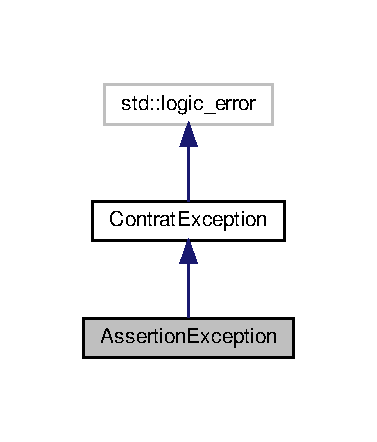
\includegraphics[width=181pt]{classAssertionException__inherit__graph}
\end{center}
\end{figure}


Collaboration diagram for Assertion\+Exception\+:\nopagebreak
\begin{figure}[H]
\begin{center}
\leavevmode
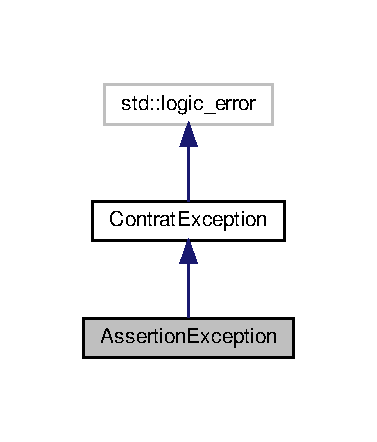
\includegraphics[width=181pt]{classAssertionException__coll__graph}
\end{center}
\end{figure}
\subsection*{Public Member Functions}
\begin{DoxyCompactItemize}
\item 
\hyperlink{classAssertionException_a93268f249b033bf4596901e50874fde6}{Assertion\+Exception} (std\+::string, unsigned int, std\+::string)
\begin{DoxyCompactList}\small\item\em Constructeur de la classe \hyperlink{classAssertionException}{Assertion\+Exception} ~\newline
 Le constructeur public \hyperlink{classAssertionException}{Assertion\+Exception}(...)initialise sa classe de base \hyperlink{classContratException}{Contrat\+Exception}. On n\textquotesingle{}a pas d\textquotesingle{}attribut local. Cette classe est intéressante pour son T\+Y\+PE lors du traitement des exceptions. \end{DoxyCompactList}\end{DoxyCompactItemize}


\subsection{Detailed Description}
Classe pour la gestion des erreurs d\textquotesingle{}assertion. 

\subsection{Constructor \& Destructor Documentation}
\mbox{\Hypertarget{classAssertionException_a93268f249b033bf4596901e50874fde6}\label{classAssertionException_a93268f249b033bf4596901e50874fde6}} 
\index{Assertion\+Exception@{Assertion\+Exception}!Assertion\+Exception@{Assertion\+Exception}}
\index{Assertion\+Exception@{Assertion\+Exception}!Assertion\+Exception@{Assertion\+Exception}}
\subsubsection{\texorpdfstring{Assertion\+Exception()}{AssertionException()}}
{\footnotesize\ttfamily Assertion\+Exception\+::\+Assertion\+Exception (\begin{DoxyParamCaption}\item[{std\+::string}]{p\+\_\+fichP,  }\item[{unsigned int}]{p\+\_\+prm\+Ligne,  }\item[{std\+::string}]{p\+\_\+exprP }\end{DoxyParamCaption})}



Constructeur de la classe \hyperlink{classAssertionException}{Assertion\+Exception} ~\newline
 Le constructeur public \hyperlink{classAssertionException}{Assertion\+Exception}(...)initialise sa classe de base \hyperlink{classContratException}{Contrat\+Exception}. On n\textquotesingle{}a pas d\textquotesingle{}attribut local. Cette classe est intéressante pour son T\+Y\+PE lors du traitement des exceptions. 


\begin{DoxyParams}{Parameters}
{\em p\+\_\+fichP} & chaîne de caractères représentant le fichier source dans lequel a eu lieu l\textquotesingle{}erreur \\
\hline
{\em p\+\_\+prm\+Ligne} & un entier représentant la ligne où a eu lieu l\textquotesingle{}erreur \\
\hline
{\em p\+\_\+exprP} & Test logique qui a échoué \\
\hline
\end{DoxyParams}


The documentation for this class was generated from the following files\+:\begin{DoxyCompactItemize}
\item 
\hyperlink{ContratException_8h}{Contrat\+Exception.\+h}\item 
\hyperlink{ContratException_8cpp}{Contrat\+Exception.\+cpp}\end{DoxyCompactItemize}

\hypertarget{classContratException}{}\section{Contrat\+Exception Class Reference}
\label{classContratException}\index{Contrat\+Exception@{Contrat\+Exception}}


Classe de base des exceptions de contrat.  




{\ttfamily \#include $<$Contrat\+Exception.\+h$>$}



Inheritance diagram for Contrat\+Exception\+:\nopagebreak
\begin{figure}[H]
\begin{center}
\leavevmode
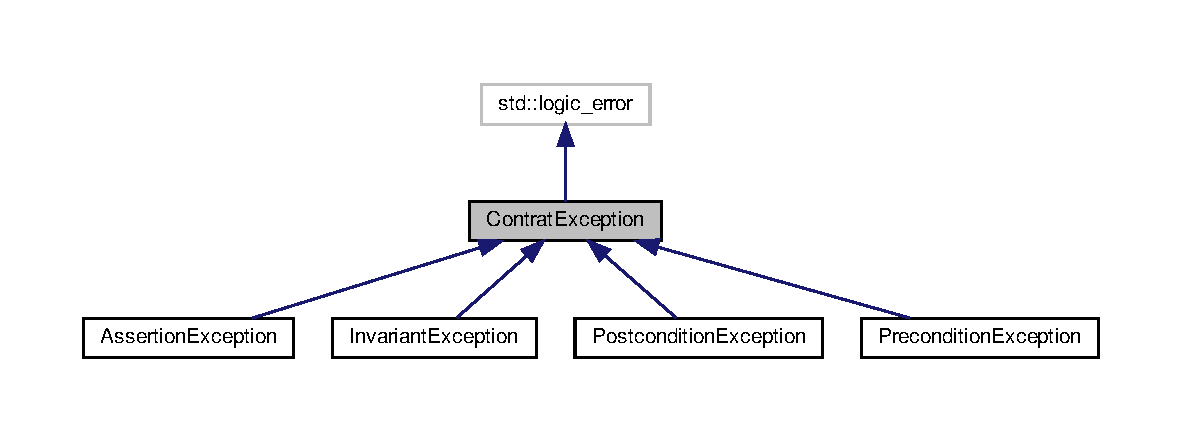
\includegraphics[width=350pt]{classContratException__inherit__graph}
\end{center}
\end{figure}


Collaboration diagram for Contrat\+Exception\+:\nopagebreak
\begin{figure}[H]
\begin{center}
\leavevmode
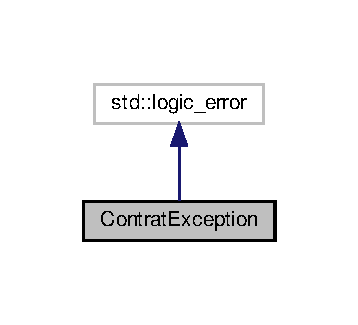
\includegraphics[width=172pt]{classContratException__coll__graph}
\end{center}
\end{figure}
\subsection*{Public Member Functions}
\begin{DoxyCompactItemize}
\item 
\hyperlink{classContratException_ad6c04fb577e960f87e010b125aa636a0}{Contrat\+Exception} (std\+::string, unsigned int, std\+::string, std\+::string)
\begin{DoxyCompactList}\small\item\em Constructeur de la classe de base \hyperlink{classContratException}{Contrat\+Exception}. \end{DoxyCompactList}\item 
std\+::string \hyperlink{classContratException_a59c9ed58985dcdd70af4ee50b2937707}{req\+Texte\+Exception} () const
\begin{DoxyCompactList}\small\item\em Construit le texte complet relié à l\textquotesingle{}exception de contrat. \end{DoxyCompactList}\end{DoxyCompactItemize}


\subsection{Detailed Description}
Classe de base des exceptions de contrat. 

\subsection{Constructor \& Destructor Documentation}
\mbox{\Hypertarget{classContratException_ad6c04fb577e960f87e010b125aa636a0}\label{classContratException_ad6c04fb577e960f87e010b125aa636a0}} 
\index{Contrat\+Exception@{Contrat\+Exception}!Contrat\+Exception@{Contrat\+Exception}}
\index{Contrat\+Exception@{Contrat\+Exception}!Contrat\+Exception@{Contrat\+Exception}}
\subsubsection{\texorpdfstring{Contrat\+Exception()}{ContratException()}}
{\footnotesize\ttfamily Contrat\+Exception\+::\+Contrat\+Exception (\begin{DoxyParamCaption}\item[{std\+::string}]{p\+\_\+fichP,  }\item[{unsigned int}]{p\+\_\+prm\+Ligne,  }\item[{std\+::string}]{p\+\_\+exprP,  }\item[{std\+::string}]{p\+\_\+msgP }\end{DoxyParamCaption})}



Constructeur de la classe de base \hyperlink{classContratException}{Contrat\+Exception}. 


\begin{DoxyParams}{Parameters}
{\em p\+\_\+fichP} & chaîne de caractères représentant le fichier source dans lequel a eu lieu l\textquotesingle{}erreur \\
\hline
{\em p\+\_\+prm\+Ligne} & un entier représentant la ligne où a eu lieu l\textquotesingle{}erreur \\
\hline
{\em p\+\_\+msgP} & Message décrivant l\textquotesingle{}erreur \\
\hline
{\em p\+\_\+exprP} & Test logique qui a échoué \\
\hline
\end{DoxyParams}


\subsection{Member Function Documentation}
\mbox{\Hypertarget{classContratException_a59c9ed58985dcdd70af4ee50b2937707}\label{classContratException_a59c9ed58985dcdd70af4ee50b2937707}} 
\index{Contrat\+Exception@{Contrat\+Exception}!req\+Texte\+Exception@{req\+Texte\+Exception}}
\index{req\+Texte\+Exception@{req\+Texte\+Exception}!Contrat\+Exception@{Contrat\+Exception}}
\subsubsection{\texorpdfstring{req\+Texte\+Exception()}{reqTexteException()}}
{\footnotesize\ttfamily std\+::string Contrat\+Exception\+::req\+Texte\+Exception (\begin{DoxyParamCaption}{ }\end{DoxyParamCaption}) const}



Construit le texte complet relié à l\textquotesingle{}exception de contrat. 

\begin{DoxyReturn}{Returns}
une chaîne de caractères correspondant à l\textquotesingle{}exception 
\end{DoxyReturn}


The documentation for this class was generated from the following files\+:\begin{DoxyCompactItemize}
\item 
\hyperlink{ContratException_8h}{Contrat\+Exception.\+h}\item 
\hyperlink{ContratException_8cpp}{Contrat\+Exception.\+cpp}\end{DoxyCompactItemize}

\hypertarget{classutil_1_1Date}{}\section{util\+:\+:Date Class Reference}
\label{classutil_1_1Date}\index{util\+::\+Date@{util\+::\+Date}}


Cette classe sert au maintien et à la manipulation des dates.  




{\ttfamily \#include $<$Date.\+h$>$}

\subsection*{Public Member Functions}
\begin{DoxyCompactItemize}
\item 
\mbox{\Hypertarget{classutil_1_1Date_a03f7ca00aa80f113bc7c0ebfbd769f54}\label{classutil_1_1Date_a03f7ca00aa80f113bc7c0ebfbd769f54}} 
\hyperlink{classutil_1_1Date_a03f7ca00aa80f113bc7c0ebfbd769f54}{Date} ()
\begin{DoxyCompactList}\small\item\em constructeur par défaut ~\newline
La date prise par défaut est la date du système \end{DoxyCompactList}\item 
\hyperlink{classutil_1_1Date_a06b8340e5beed84c885c89d41a750330}{Date} (long p\+\_\+jour, long p\+\_\+mois, long p\+\_\+annee)
\begin{DoxyCompactList}\small\item\em constructeur avec paramètres On construit un objet \hyperlink{classutil_1_1Date}{Date} à partir de valeurs passées en paramètres. Les attributs sont assignés seulement si la date est considérée comme valide. Autrement, une erreur d\textquotesingle{}assertion est générée. \end{DoxyCompactList}\item 
void \hyperlink{classutil_1_1Date_ab82f59d834f60b929ca130f15e5279c3}{asg\+Date} (long p\+\_\+jour, long p\+\_\+mois, long p\+\_\+annee)
\begin{DoxyCompactList}\small\item\em Assigne une date à l\textquotesingle{}objet courant. \end{DoxyCompactList}\item 
bool \hyperlink{classutil_1_1Date_a7788599612a71d89126d649fdaaced3d}{ajoute\+Nb\+Jour} (long p\+\_\+nbjour)
\begin{DoxyCompactList}\small\item\em Ajoute ou retire un certain nombre de jours à la date courante. \end{DoxyCompactList}\item 
long \hyperlink{classutil_1_1Date_aa2b8c7a6e23e9244a5bac8342484d3b8}{req\+Jour} () const
\begin{DoxyCompactList}\small\item\em retourne le jour de la date \end{DoxyCompactList}\item 
long \hyperlink{classutil_1_1Date_a8002c391b812945da68b16cb4a424460}{req\+Mois} () const
\begin{DoxyCompactList}\small\item\em retourne le mois de la date \end{DoxyCompactList}\item 
long \hyperlink{classutil_1_1Date_aa7c4b428456da55a2e3769e93ad9bb8d}{req\+Annee} () const
\begin{DoxyCompactList}\small\item\em retourne l\textquotesingle{}année de la date \end{DoxyCompactList}\item 
long \hyperlink{classutil_1_1Date_a9e76af410b6be9ac4ea9ab4df5797847}{req\+Jour\+Annee} () const
\begin{DoxyCompactList}\small\item\em retourne le ième jour de l\textquotesingle{}année correspondant au jour de la date \end{DoxyCompactList}\item 
std\+::string \hyperlink{classutil_1_1Date_ad92d1e9c4d570c5f31a8e06cf2e1ae8c}{req\+Date\+Formatee} () const
\begin{DoxyCompactList}\small\item\em retourne une date formatée dans une chaîne de caracères (string) \end{DoxyCompactList}\item 
bool \hyperlink{classutil_1_1Date_a8114f8e40cee24e1d7a58b910e8f4637}{operator==} (const \hyperlink{classutil_1_1Date}{Date} \&p\+\_\+date) const
\begin{DoxyCompactList}\small\item\em surcharge de l\textquotesingle{}opérateur == \end{DoxyCompactList}\item 
bool \hyperlink{classutil_1_1Date_aefcf8a7520711f783fb0241d460480c5}{operator$<$} (const \hyperlink{classutil_1_1Date}{Date} \&p\+\_\+date) const
\begin{DoxyCompactList}\small\item\em surcharge de l\textquotesingle{}opérateur $<$ \end{DoxyCompactList}\item 
bool \hyperlink{classutil_1_1Date_af65a0fddef5326badc11d48d1dd253cd}{operator$<$=} (const \hyperlink{classutil_1_1Date}{Date} \&p\+\_\+date) const
\begin{DoxyCompactList}\small\item\em surcharge de l\textquotesingle{}opérateur $<$= \end{DoxyCompactList}\item 
int \hyperlink{classutil_1_1Date_af12f2c545070b5e2b397be5379c5c3fd}{operator-\/} (const \hyperlink{classutil_1_1Date}{Date} \&p\+\_\+date) const
\begin{DoxyCompactList}\small\item\em retourne le nombre de jours entre deux dates \end{DoxyCompactList}\end{DoxyCompactItemize}
\subsection*{Static Public Member Functions}
\begin{DoxyCompactItemize}
\item 
static bool \hyperlink{classutil_1_1Date_af80efec6a713cdb671d8b23c3e8c4efb}{est\+Bissextile} (long p\+\_\+annee)
\begin{DoxyCompactList}\small\item\em Déterminer si une année est bissextile ou non. \end{DoxyCompactList}\item 
static bool \hyperlink{classutil_1_1Date_af4b4dde01395754245a42483358cb538}{valider\+Date} (long p\+\_\+jour, long p\+\_\+mois, long p\+\_\+annee)
\begin{DoxyCompactList}\small\item\em Vérifie la validité d\textquotesingle{}une date. \end{DoxyCompactList}\end{DoxyCompactItemize}
\subsection*{Friends}
\begin{DoxyCompactItemize}
\item 
\mbox{\Hypertarget{classutil_1_1Date_ab01372aff5a2aa1d5f5bab251bb7951c}\label{classutil_1_1Date_ab01372aff5a2aa1d5f5bab251bb7951c}} 
std\+::ostream \& {\bfseries operator$<$$<$} (std\+::ostream \&p\+\_\+os, const \hyperlink{classutil_1_1Date}{Date} \&p\+\_\+date)
\end{DoxyCompactItemize}
\subsection*{Related Functions}
(Note that these are not member functions.) \begin{DoxyCompactItemize}
\item 
ostream \& \hyperlink{classutil_1_1Date_a3b88f9a1692395518a45b282a19f10e8}{operator$<$$<$} (ostream \&p\+\_\+os, const \hyperlink{classutil_1_1Date}{Date} \&p\+\_\+date)
\begin{DoxyCompactList}\small\item\em surcharge de la fonction $<$$<$ d\textquotesingle{}écriture dans un flux de sortie \end{DoxyCompactList}\end{DoxyCompactItemize}


\subsection{Detailed Description}
Cette classe sert au maintien et à la manipulation des dates. 

La classe maintient dans un état cohérent ces renseignements. Elle valide ce qu\textquotesingle{}on veut lui assigner. 

Cette classe peut aussi servir à prendre la date courante du système et à faire des calculs avec des dates. 

La classe n\textquotesingle{}accepte que des dates valides, c\textquotesingle{}est la responsabilité de l\textquotesingle{}utilisateur de la classe de s\textquotesingle{}en assurer. 

Attributs\+: time\+\_\+t m\+\_\+temps Nombre de secondes écoulé depuis le premier janvier 1970 

time\+\_\+t m\+\_\+temps pour long m\+\_\+temps \begin{DoxyInvariant}{Invariant}
m\+\_\+temps $>$= 1er janvier 1970 et $>$= au 31 décembre 2037 

La validité peut être vérifiée avec la méthode statique bool Date\+::verifier\+Date(jour, mois, annee). 
\end{DoxyInvariant}


\subsection{Constructor \& Destructor Documentation}
\mbox{\Hypertarget{classutil_1_1Date_a06b8340e5beed84c885c89d41a750330}\label{classutil_1_1Date_a06b8340e5beed84c885c89d41a750330}} 
\index{util\+::\+Date@{util\+::\+Date}!Date@{Date}}
\index{Date@{Date}!util\+::\+Date@{util\+::\+Date}}
\subsubsection{\texorpdfstring{Date()}{Date()}}
{\footnotesize\ttfamily util\+::\+Date\+::\+Date (\begin{DoxyParamCaption}\item[{long}]{p\+\_\+jour,  }\item[{long}]{p\+\_\+mois,  }\item[{long}]{p\+\_\+annee }\end{DoxyParamCaption})}



constructeur avec paramètres On construit un objet \hyperlink{classutil_1_1Date}{Date} à partir de valeurs passées en paramètres. Les attributs sont assignés seulement si la date est considérée comme valide. Autrement, une erreur d\textquotesingle{}assertion est générée. 


\begin{DoxyParams}[1]{Parameters}
\mbox{\tt in}  & {\em p\+\_\+jour} & est un entier long qui représente le jour de la date \\
\hline
\mbox{\tt in}  & {\em p\+\_\+mois} & est un entier long qui représente le mois de la date \\
\hline
\mbox{\tt in}  & {\em p\+\_\+annee} & est un entier long qui représente l\textquotesingle{}année de la date \\
\hline
\end{DoxyParams}
\begin{DoxyPrecond}{Precondition}
p\+\_\+jour, p\+\_\+mois, p\+\_\+annee doivent correspondre à une date valide 
\end{DoxyPrecond}
\begin{DoxyPostcond}{Postcondition}
l\textquotesingle{}objet construit a été initialisé à partir des entiers passés en paramètres 
\end{DoxyPostcond}


\subsection{Member Function Documentation}
\mbox{\Hypertarget{classutil_1_1Date_a7788599612a71d89126d649fdaaced3d}\label{classutil_1_1Date_a7788599612a71d89126d649fdaaced3d}} 
\index{util\+::\+Date@{util\+::\+Date}!ajoute\+Nb\+Jour@{ajoute\+Nb\+Jour}}
\index{ajoute\+Nb\+Jour@{ajoute\+Nb\+Jour}!util\+::\+Date@{util\+::\+Date}}
\subsubsection{\texorpdfstring{ajoute\+Nb\+Jour()}{ajouteNbJour()}}
{\footnotesize\ttfamily bool util\+::\+Date\+::ajoute\+Nb\+Jour (\begin{DoxyParamCaption}\item[{long}]{p\+\_\+nb\+Jour }\end{DoxyParamCaption})}



Ajoute ou retire un certain nombre de jours à la date courante. 


\begin{DoxyParams}{Parameters}
{\em p\+\_\+nb\+Jour} & est une entier long qui représente le nombre de jours à ajouter ou à soustraire s\textquotesingle{}il est négatif \\
\hline
\end{DoxyParams}
\begin{DoxyReturn}{Returns}
un booléen qui indique si l\textquotesingle{}opération a réussi ou non 
\end{DoxyReturn}
\mbox{\Hypertarget{classutil_1_1Date_ab82f59d834f60b929ca130f15e5279c3}\label{classutil_1_1Date_ab82f59d834f60b929ca130f15e5279c3}} 
\index{util\+::\+Date@{util\+::\+Date}!asg\+Date@{asg\+Date}}
\index{asg\+Date@{asg\+Date}!util\+::\+Date@{util\+::\+Date}}
\subsubsection{\texorpdfstring{asg\+Date()}{asgDate()}}
{\footnotesize\ttfamily void util\+::\+Date\+::asg\+Date (\begin{DoxyParamCaption}\item[{long}]{p\+\_\+jour,  }\item[{long}]{p\+\_\+mois,  }\item[{long}]{p\+\_\+annee }\end{DoxyParamCaption})}



Assigne une date à l\textquotesingle{}objet courant. 


\begin{DoxyParams}[1]{Parameters}
\mbox{\tt in}  & {\em p\+\_\+jour} & est un entier long qui représente le jour de la date \\
\hline
\mbox{\tt in}  & {\em p\+\_\+mois} & est un entier long qui représente le mois de la date \\
\hline
\mbox{\tt in}  & {\em p\+\_\+annee} & est un entier long qui représente l\textquotesingle{}année de la date \\
\hline
\end{DoxyParams}
\begin{DoxyPrecond}{Precondition}
p\+\_\+jour, p\+\_\+mois, p\+\_\+annee doivent correspondre à une date valide 
\end{DoxyPrecond}
\begin{DoxyPostcond}{Postcondition}
l\textquotesingle{}objet a été assigné à partir des entiers passés en paramètres 
\end{DoxyPostcond}
\mbox{\Hypertarget{classutil_1_1Date_af80efec6a713cdb671d8b23c3e8c4efb}\label{classutil_1_1Date_af80efec6a713cdb671d8b23c3e8c4efb}} 
\index{util\+::\+Date@{util\+::\+Date}!est\+Bissextile@{est\+Bissextile}}
\index{est\+Bissextile@{est\+Bissextile}!util\+::\+Date@{util\+::\+Date}}
\subsubsection{\texorpdfstring{est\+Bissextile()}{estBissextile()}}
{\footnotesize\ttfamily bool util\+::\+Date\+::est\+Bissextile (\begin{DoxyParamCaption}\item[{long}]{p\+\_\+annee }\end{DoxyParamCaption})\hspace{0.3cm}{\ttfamily [static]}}



Déterminer si une année est bissextile ou non. 


\begin{DoxyParams}[1]{Parameters}
\mbox{\tt in}  & {\em p\+\_\+annee} & un entier long qui représente l\textquotesingle{}année à vérifier \\
\hline
\end{DoxyParams}
\begin{DoxyReturn}{Returns}
est\+Bissextile un booléen qui a la valeur true si l\textquotesingle{}année est bissextile et false sinon 
\end{DoxyReturn}
\mbox{\Hypertarget{classutil_1_1Date_af12f2c545070b5e2b397be5379c5c3fd}\label{classutil_1_1Date_af12f2c545070b5e2b397be5379c5c3fd}} 
\index{util\+::\+Date@{util\+::\+Date}!operator-\/@{operator-\/}}
\index{operator-\/@{operator-\/}!util\+::\+Date@{util\+::\+Date}}
\subsubsection{\texorpdfstring{operator-\/()}{operator-()}}
{\footnotesize\ttfamily int util\+::\+Date\+::operator-\/ (\begin{DoxyParamCaption}\item[{const \hyperlink{classutil_1_1Date}{Date} \&}]{p\+\_\+date }\end{DoxyParamCaption}) const}



retourne le nombre de jours entre deux dates 


\begin{DoxyParams}[1]{Parameters}
\mbox{\tt in}  & {\em p\+\_\+date} & à soustraire à la date courante \\
\hline
\end{DoxyParams}
\begin{DoxyReturn}{Returns}
un entier qui représente le nombre de jours entre la date courante et celle passée en paramètre 
\end{DoxyReturn}
\mbox{\Hypertarget{classutil_1_1Date_aefcf8a7520711f783fb0241d460480c5}\label{classutil_1_1Date_aefcf8a7520711f783fb0241d460480c5}} 
\index{util\+::\+Date@{util\+::\+Date}!operator$<$@{operator$<$}}
\index{operator$<$@{operator$<$}!util\+::\+Date@{util\+::\+Date}}
\subsubsection{\texorpdfstring{operator$<$()}{operator<()}}
{\footnotesize\ttfamily bool util\+::\+Date\+::operator$<$ (\begin{DoxyParamCaption}\item[{const \hyperlink{classutil_1_1Date}{Date} \&}]{p\+\_\+date }\end{DoxyParamCaption}) const}



surcharge de l\textquotesingle{}opérateur $<$ 


\begin{DoxyParams}[1]{Parameters}
\mbox{\tt in}  & {\em p\+\_\+date} & à comparer à la date courante \\
\hline
\end{DoxyParams}
\begin{DoxyReturn}{Returns}
un booléen indiquant si la date courante est plus petite que la date passée en paramètre 
\end{DoxyReturn}
\mbox{\Hypertarget{classutil_1_1Date_af65a0fddef5326badc11d48d1dd253cd}\label{classutil_1_1Date_af65a0fddef5326badc11d48d1dd253cd}} 
\index{util\+::\+Date@{util\+::\+Date}!operator$<$=@{operator$<$=}}
\index{operator$<$=@{operator$<$=}!util\+::\+Date@{util\+::\+Date}}
\subsubsection{\texorpdfstring{operator$<$=()}{operator<=()}}
{\footnotesize\ttfamily bool util\+::\+Date\+::operator$<$= (\begin{DoxyParamCaption}\item[{const \hyperlink{classutil_1_1Date}{Date} \&}]{p\+\_\+date }\end{DoxyParamCaption}) const}



surcharge de l\textquotesingle{}opérateur $<$= 


\begin{DoxyParams}[1]{Parameters}
\mbox{\tt in}  & {\em p\+\_\+date} & à comparer à la date courante \\
\hline
\end{DoxyParams}
\begin{DoxyReturn}{Returns}
un booléen indiquant si la date courante est plus petite ou égale que la date passée en paramètre 
\end{DoxyReturn}
\mbox{\Hypertarget{classutil_1_1Date_a8114f8e40cee24e1d7a58b910e8f4637}\label{classutil_1_1Date_a8114f8e40cee24e1d7a58b910e8f4637}} 
\index{util\+::\+Date@{util\+::\+Date}!operator==@{operator==}}
\index{operator==@{operator==}!util\+::\+Date@{util\+::\+Date}}
\subsubsection{\texorpdfstring{operator==()}{operator==()}}
{\footnotesize\ttfamily bool util\+::\+Date\+::operator== (\begin{DoxyParamCaption}\item[{const \hyperlink{classutil_1_1Date}{Date} \&}]{p\+\_\+date }\end{DoxyParamCaption}) const}



surcharge de l\textquotesingle{}opérateur == 


\begin{DoxyParams}[1]{Parameters}
\mbox{\tt in}  & {\em p\+\_\+date} & à comparer à la date courante \\
\hline
\end{DoxyParams}
\begin{DoxyReturn}{Returns}
un booléen indiquant si les deux dates sont égales ou non 
\end{DoxyReturn}
\mbox{\Hypertarget{classutil_1_1Date_aa7c4b428456da55a2e3769e93ad9bb8d}\label{classutil_1_1Date_aa7c4b428456da55a2e3769e93ad9bb8d}} 
\index{util\+::\+Date@{util\+::\+Date}!req\+Annee@{req\+Annee}}
\index{req\+Annee@{req\+Annee}!util\+::\+Date@{util\+::\+Date}}
\subsubsection{\texorpdfstring{req\+Annee()}{reqAnnee()}}
{\footnotesize\ttfamily long util\+::\+Date\+::req\+Annee (\begin{DoxyParamCaption}{ }\end{DoxyParamCaption}) const}



retourne l\textquotesingle{}année de la date 

\begin{DoxyReturn}{Returns}
un entier long qui représente l\textquotesingle{}année de la date 
\end{DoxyReturn}
\mbox{\Hypertarget{classutil_1_1Date_ad92d1e9c4d570c5f31a8e06cf2e1ae8c}\label{classutil_1_1Date_ad92d1e9c4d570c5f31a8e06cf2e1ae8c}} 
\index{util\+::\+Date@{util\+::\+Date}!req\+Date\+Formatee@{req\+Date\+Formatee}}
\index{req\+Date\+Formatee@{req\+Date\+Formatee}!util\+::\+Date@{util\+::\+Date}}
\subsubsection{\texorpdfstring{req\+Date\+Formatee()}{reqDateFormatee()}}
{\footnotesize\ttfamily string util\+::\+Date\+::req\+Date\+Formatee (\begin{DoxyParamCaption}{ }\end{DoxyParamCaption}) const}



retourne une date formatée dans une chaîne de caracères (string) 

\begin{DoxyReturn}{Returns}
la date formatée dans une chaîne de caractères 
\end{DoxyReturn}
\mbox{\Hypertarget{classutil_1_1Date_aa2b8c7a6e23e9244a5bac8342484d3b8}\label{classutil_1_1Date_aa2b8c7a6e23e9244a5bac8342484d3b8}} 
\index{util\+::\+Date@{util\+::\+Date}!req\+Jour@{req\+Jour}}
\index{req\+Jour@{req\+Jour}!util\+::\+Date@{util\+::\+Date}}
\subsubsection{\texorpdfstring{req\+Jour()}{reqJour()}}
{\footnotesize\ttfamily long util\+::\+Date\+::req\+Jour (\begin{DoxyParamCaption}{ }\end{DoxyParamCaption}) const}



retourne le jour de la date 

\begin{DoxyReturn}{Returns}
un entier long qui représente le jour de la date 
\end{DoxyReturn}
\mbox{\Hypertarget{classutil_1_1Date_a9e76af410b6be9ac4ea9ab4df5797847}\label{classutil_1_1Date_a9e76af410b6be9ac4ea9ab4df5797847}} 
\index{util\+::\+Date@{util\+::\+Date}!req\+Jour\+Annee@{req\+Jour\+Annee}}
\index{req\+Jour\+Annee@{req\+Jour\+Annee}!util\+::\+Date@{util\+::\+Date}}
\subsubsection{\texorpdfstring{req\+Jour\+Annee()}{reqJourAnnee()}}
{\footnotesize\ttfamily long util\+::\+Date\+::req\+Jour\+Annee (\begin{DoxyParamCaption}{ }\end{DoxyParamCaption}) const}



retourne le ième jour de l\textquotesingle{}année correspondant au jour de la date 

\begin{DoxyReturn}{Returns}
un entier long qui représente le ième jour de l\textquotesingle{}année 
\end{DoxyReturn}
\mbox{\Hypertarget{classutil_1_1Date_a8002c391b812945da68b16cb4a424460}\label{classutil_1_1Date_a8002c391b812945da68b16cb4a424460}} 
\index{util\+::\+Date@{util\+::\+Date}!req\+Mois@{req\+Mois}}
\index{req\+Mois@{req\+Mois}!util\+::\+Date@{util\+::\+Date}}
\subsubsection{\texorpdfstring{req\+Mois()}{reqMois()}}
{\footnotesize\ttfamily long util\+::\+Date\+::req\+Mois (\begin{DoxyParamCaption}{ }\end{DoxyParamCaption}) const}



retourne le mois de la date 

\begin{DoxyReturn}{Returns}
un entier long qui représente le mois de la date 
\end{DoxyReturn}
\mbox{\Hypertarget{classutil_1_1Date_af4b4dde01395754245a42483358cb538}\label{classutil_1_1Date_af4b4dde01395754245a42483358cb538}} 
\index{util\+::\+Date@{util\+::\+Date}!valider\+Date@{valider\+Date}}
\index{valider\+Date@{valider\+Date}!util\+::\+Date@{util\+::\+Date}}
\subsubsection{\texorpdfstring{valider\+Date()}{validerDate()}}
{\footnotesize\ttfamily bool util\+::\+Date\+::valider\+Date (\begin{DoxyParamCaption}\item[{long}]{p\+\_\+jour,  }\item[{long}]{p\+\_\+mois,  }\item[{long}]{p\+\_\+annee }\end{DoxyParamCaption})\hspace{0.3cm}{\ttfamily [static]}}



Vérifie la validité d\textquotesingle{}une date. 


\begin{DoxyParams}[1]{Parameters}
\mbox{\tt in}  & {\em p\+\_\+jour} & un entier long représentant le jour de la date \\
\hline
\mbox{\tt in}  & {\em p\+\_\+mois} & un entier long représentant le mois de la date \\
\hline
\mbox{\tt in}  & {\em p\+\_\+annee} & un entier long représentant l\textquotesingle{}année de la date \\
\hline
\end{DoxyParams}
\begin{DoxyReturn}{Returns}
un booléen indiquant si la date est valide ou non 
\end{DoxyReturn}


\subsection{Friends And Related Function Documentation}
\mbox{\Hypertarget{classutil_1_1Date_a3b88f9a1692395518a45b282a19f10e8}\label{classutil_1_1Date_a3b88f9a1692395518a45b282a19f10e8}} 
\index{util\+::\+Date@{util\+::\+Date}!operator$<$$<$@{operator$<$$<$}}
\index{operator$<$$<$@{operator$<$$<$}!util\+::\+Date@{util\+::\+Date}}
\subsubsection{\texorpdfstring{operator$<$$<$()}{operator<<()}}
{\footnotesize\ttfamily ostream \& operator$<$$<$ (\begin{DoxyParamCaption}\item[{ostream \&}]{p\+\_\+os,  }\item[{const \hyperlink{classutil_1_1Date}{Date} \&}]{p\+\_\+date }\end{DoxyParamCaption})\hspace{0.3cm}{\ttfamily [related]}}



surcharge de la fonction $<$$<$ d\textquotesingle{}écriture dans un flux de sortie 


\begin{DoxyParams}[1]{Parameters}
\mbox{\tt in}  & {\em p\+\_\+os} & un flux de sortie dans laquelle on va écrire \\
\hline
\mbox{\tt in}  & {\em p\+\_\+date} & sortie dans le flux \\
\hline
\end{DoxyParams}
\begin{DoxyReturn}{Returns}
le flux dans lequel on a écrit la date, ceci pour les appels en cascade 
\end{DoxyReturn}


The documentation for this class was generated from the following files\+:\begin{DoxyCompactItemize}
\item 
\hyperlink{Date_8h}{Date.\+h}\item 
\hyperlink{Date_8cpp}{Date.\+cpp}\end{DoxyCompactItemize}

\hypertarget{classhockey_1_1Entraineur}{}\section{hockey\+:\+:Entraineur Class Reference}
\label{classhockey_1_1Entraineur}\index{hockey\+::\+Entraineur@{hockey\+::\+Entraineur}}


Cette classe sert au maintien et à la manipulation des entraineurs. Elle hérite de la classe \hyperlink{classhockey_1_1Personne}{Personne}.  




{\ttfamily \#include $<$Entraineur.\+h$>$}



Inheritance diagram for hockey\+:\+:Entraineur\+:\nopagebreak
\begin{figure}[H]
\begin{center}
\leavevmode
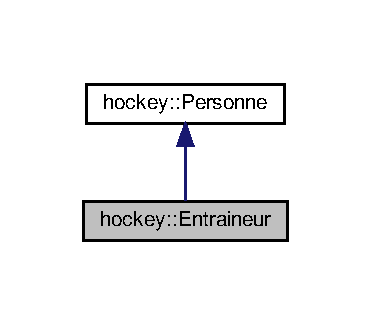
\includegraphics[width=178pt]{classhockey_1_1Entraineur__inherit__graph}
\end{center}
\end{figure}


Collaboration diagram for hockey\+:\+:Entraineur\+:\nopagebreak
\begin{figure}[H]
\begin{center}
\leavevmode
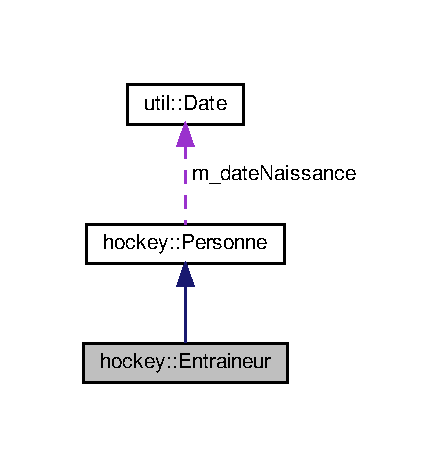
\includegraphics[width=211pt]{classhockey_1_1Entraineur__coll__graph}
\end{center}
\end{figure}
\subsection*{Public Member Functions}
\begin{DoxyCompactItemize}
\item 
\hyperlink{classhockey_1_1Entraineur_a707fdafbb52daf320baf757f7d7c460f}{Entraineur} (std\+::string p\+\_\+nom, std\+::string p\+\_\+prenom, const \hyperlink{classutil_1_1Date}{util\+::\+Date} \&p\+\_\+date\+Naissance, std\+::string p\+\_\+telephone, std\+::string p\+\_\+num\+R\+A\+MQ, char p\+\_\+sexe)
\begin{DoxyCompactList}\small\item\em Constructeur de la classe entraîneur avec des paramètres en entrée. \end{DoxyCompactList}\item 
\mbox{\Hypertarget{classhockey_1_1Entraineur_a4dff2cf754acea2fbc3a510146618de9}\label{classhockey_1_1Entraineur_a4dff2cf754acea2fbc3a510146618de9}} 
\hyperlink{classhockey_1_1Entraineur_a4dff2cf754acea2fbc3a510146618de9}{Entraineur} ()
\begin{DoxyCompactList}\small\item\em Constructeur de la classe entraîneur sans paramètre d\textquotesingle{}entrée. Ce constructeur permet de retourner une erreur de précondition si le constructeur vide par défaut est utilisé. \end{DoxyCompactList}\item 
const std\+::string \& \hyperlink{classhockey_1_1Entraineur_a7f9bb4ef1197e785be0cd7e506f26bbd}{req\+Num\+R\+A\+MQ} () const
\begin{DoxyCompactList}\small\item\em Méthode permettant de retourner le numéro de R\+A\+MQ de l\textquotesingle{}entraîneur. \end{DoxyCompactList}\item 
const char \& \hyperlink{classhockey_1_1Entraineur_a8bd3cd9717f896085b74782e5b1170fc}{req\+Sexe} () const
\begin{DoxyCompactList}\small\item\em Méthode permettant de retourner le sexe de l\textquotesingle{}entraîneur. \end{DoxyCompactList}\item 
virtual std\+::string \hyperlink{classhockey_1_1Entraineur_a376149c10b8541c45d703682d41d80f3}{req\+Personne\+Formate} () const
\begin{DoxyCompactList}\small\item\em Méthode permettant de retourner les informations de l\textquotesingle{}entraîneur. \end{DoxyCompactList}\item 
virtual \hyperlink{classhockey_1_1Personne}{Personne} $\ast$ \hyperlink{classhockey_1_1Entraineur_a734eb3d04a6209542fbfc989c398613e}{clone} () const
\begin{DoxyCompactList}\small\item\em Méthode permettant de créer une nouvelle instance de l\textquotesingle{}entraîneur. \end{DoxyCompactList}\item 
\mbox{\Hypertarget{classhockey_1_1Entraineur_a5146ae4be0b4ce34d8056cb0a012d5be}\label{classhockey_1_1Entraineur_a5146ae4be0b4ce34d8056cb0a012d5be}} 
virtual \hyperlink{classhockey_1_1Entraineur_a5146ae4be0b4ce34d8056cb0a012d5be}{$\sim$\+Entraineur} ()
\begin{DoxyCompactList}\small\item\em Destructeur de la classe \hyperlink{classhockey_1_1Entraineur}{Entraineur}. \end{DoxyCompactList}\end{DoxyCompactItemize}
\subsection*{Additional Inherited Members}


\subsection{Detailed Description}
Cette classe sert au maintien et à la manipulation des entraineurs. Elle hérite de la classe \hyperlink{classhockey_1_1Personne}{Personne}. 

Les valeurs qui entrent dans la classe doivent être validée à priori. 

Attributs\+: string p\+\_\+nom, string p\+\_\+prenom, Date p\+\_\+date\+Naissance, string p\+\_\+telephone, p\+\_\+num\+R\+A\+MQ, p\+\_\+sexe 

\subsection{Constructor \& Destructor Documentation}
\mbox{\Hypertarget{classhockey_1_1Entraineur_a707fdafbb52daf320baf757f7d7c460f}\label{classhockey_1_1Entraineur_a707fdafbb52daf320baf757f7d7c460f}} 
\index{hockey\+::\+Entraineur@{hockey\+::\+Entraineur}!Entraineur@{Entraineur}}
\index{Entraineur@{Entraineur}!hockey\+::\+Entraineur@{hockey\+::\+Entraineur}}
\subsubsection{\texorpdfstring{Entraineur()}{Entraineur()}}
{\footnotesize\ttfamily hockey\+::\+Entraineur\+::\+Entraineur (\begin{DoxyParamCaption}\item[{std\+::string}]{p\+\_\+nom,  }\item[{std\+::string}]{p\+\_\+prenom,  }\item[{const \hyperlink{classutil_1_1Date}{util\+::\+Date} \&}]{p\+\_\+date\+Naissance,  }\item[{std\+::string}]{p\+\_\+telephone,  }\item[{std\+::string}]{p\+\_\+num\+R\+A\+MQ,  }\item[{char}]{p\+\_\+sexe }\end{DoxyParamCaption})}



Constructeur de la classe entraîneur avec des paramètres en entrée. 


\begin{DoxyParams}[1]{Parameters}
\mbox{\tt in}  & {\em p\+\_\+nom} & un string représentant le nom de l\textquotesingle{}entraîneur \\
\hline
\mbox{\tt in}  & {\em p\+\_\+prenom} & un string représentant le prénom de l\textquotesingle{}entraîneur \\
\hline
\mbox{\tt in}  & {\em p\+\_\+date\+Naissance} & un objet Date représentant la date de naissance de l\textquotesingle{}entraîneur \\
\hline
\mbox{\tt in}  & {\em p\+\_\+telephone} & un string représentant le numéro de téléphone de l\textquotesingle{}entraîneur \\
\hline
\mbox{\tt in}  & {\em p\+\_\+num\+R\+A\+MQ} & un string représentant le numéro de R\+A\+MQ de l\textquotesingle{}entraîneur \\
\hline
\mbox{\tt in}  & {\em p\+\_\+sexe} & un char représentant le sexe de l\textquotesingle{}entraîneur \\
\hline
\end{DoxyParams}
\begin{DoxyPrecond}{Precondition}
Tous les paramètres en entrée doivent être valide pour une personne standard. 

Le numéro de R\+A\+MQ de l\textquotesingle{}entraîneur doit être valide avec les infos de l\textquotesingle{}entraîneur et avoir un format valide 

Le sexe de l\textquotesingle{}entraîneur doit être \textquotesingle{}m\textquotesingle{} ou \textquotesingle{}M\textquotesingle{} pour homme et \textquotesingle{}f\textquotesingle{} ou \textquotesingle{}F\textquotesingle{} pour femme. 
\end{DoxyPrecond}
\begin{DoxyInvariant}{Invariant}
Les invariants de l\textquotesingle{}entraîneur sont les mêmes que ceux d\textquotesingle{}une personne standard. 

L\textquotesingle{}entraîneur doit également avoir un sexe valide et un numéro de R\+A\+MQ valide. 
\end{DoxyInvariant}


\subsection{Member Function Documentation}
\mbox{\Hypertarget{classhockey_1_1Entraineur_a734eb3d04a6209542fbfc989c398613e}\label{classhockey_1_1Entraineur_a734eb3d04a6209542fbfc989c398613e}} 
\index{hockey\+::\+Entraineur@{hockey\+::\+Entraineur}!clone@{clone}}
\index{clone@{clone}!hockey\+::\+Entraineur@{hockey\+::\+Entraineur}}
\subsubsection{\texorpdfstring{clone()}{clone()}}
{\footnotesize\ttfamily \hyperlink{classhockey_1_1Personne}{Personne} $\ast$ hockey\+::\+Entraineur\+::clone (\begin{DoxyParamCaption}{ }\end{DoxyParamCaption}) const\hspace{0.3cm}{\ttfamily [virtual]}}



Méthode permettant de créer une nouvelle instance de l\textquotesingle{}entraîneur. 

\begin{DoxyReturn}{Returns}
un pointeur vers la nouvelle instance de l\textquotesingle{}entraîneur. 
\end{DoxyReturn}


Implements \hyperlink{classhockey_1_1Personne}{hockey\+::\+Personne}.

\mbox{\Hypertarget{classhockey_1_1Entraineur_a7f9bb4ef1197e785be0cd7e506f26bbd}\label{classhockey_1_1Entraineur_a7f9bb4ef1197e785be0cd7e506f26bbd}} 
\index{hockey\+::\+Entraineur@{hockey\+::\+Entraineur}!req\+Num\+R\+A\+MQ@{req\+Num\+R\+A\+MQ}}
\index{req\+Num\+R\+A\+MQ@{req\+Num\+R\+A\+MQ}!hockey\+::\+Entraineur@{hockey\+::\+Entraineur}}
\subsubsection{\texorpdfstring{req\+Num\+R\+A\+M\+Q()}{reqNumRAMQ()}}
{\footnotesize\ttfamily const string \& hockey\+::\+Entraineur\+::req\+Num\+R\+A\+MQ (\begin{DoxyParamCaption}{ }\end{DoxyParamCaption}) const}



Méthode permettant de retourner le numéro de R\+A\+MQ de l\textquotesingle{}entraîneur. 

\begin{DoxyReturn}{Returns}
un string représentant le numéro de R\+A\+MQ de l\textquotesingle{}entraîneur. 
\end{DoxyReturn}
\mbox{\Hypertarget{classhockey_1_1Entraineur_a376149c10b8541c45d703682d41d80f3}\label{classhockey_1_1Entraineur_a376149c10b8541c45d703682d41d80f3}} 
\index{hockey\+::\+Entraineur@{hockey\+::\+Entraineur}!req\+Personne\+Formate@{req\+Personne\+Formate}}
\index{req\+Personne\+Formate@{req\+Personne\+Formate}!hockey\+::\+Entraineur@{hockey\+::\+Entraineur}}
\subsubsection{\texorpdfstring{req\+Personne\+Formate()}{reqPersonneFormate()}}
{\footnotesize\ttfamily string hockey\+::\+Entraineur\+::req\+Personne\+Formate (\begin{DoxyParamCaption}{ }\end{DoxyParamCaption}) const\hspace{0.3cm}{\ttfamily [virtual]}}



Méthode permettant de retourner les informations de l\textquotesingle{}entraîneur. 

\begin{DoxyReturn}{Returns}
un string représentant les informations de l\textquotesingle{}entraîneur. 
\end{DoxyReturn}


Reimplemented from \hyperlink{classhockey_1_1Personne_ae67b3d253c1fa8a090dd8040ca1e8ccc}{hockey\+::\+Personne}.

\mbox{\Hypertarget{classhockey_1_1Entraineur_a8bd3cd9717f896085b74782e5b1170fc}\label{classhockey_1_1Entraineur_a8bd3cd9717f896085b74782e5b1170fc}} 
\index{hockey\+::\+Entraineur@{hockey\+::\+Entraineur}!req\+Sexe@{req\+Sexe}}
\index{req\+Sexe@{req\+Sexe}!hockey\+::\+Entraineur@{hockey\+::\+Entraineur}}
\subsubsection{\texorpdfstring{req\+Sexe()}{reqSexe()}}
{\footnotesize\ttfamily const char \& hockey\+::\+Entraineur\+::req\+Sexe (\begin{DoxyParamCaption}{ }\end{DoxyParamCaption}) const}



Méthode permettant de retourner le sexe de l\textquotesingle{}entraîneur. 

\begin{DoxyReturn}{Returns}
un char représentant le sexe de l\textquotesingle{}entraîneur. 
\end{DoxyReturn}


The documentation for this class was generated from the following files\+:\begin{DoxyCompactItemize}
\item 
\hyperlink{Entraineur_8h}{Entraineur.\+h}\item 
Entraineur.\+cpp\end{DoxyCompactItemize}

\hypertarget{classInvariantException}{}\section{Invariant\+Exception Class Reference}
\label{classInvariantException}\index{Invariant\+Exception@{Invariant\+Exception}}


Classe pour la gestion des erreurs d\textquotesingle{}invariant.  




{\ttfamily \#include $<$Contrat\+Exception.\+h$>$}



Inheritance diagram for Invariant\+Exception\+:\nopagebreak
\begin{figure}[H]
\begin{center}
\leavevmode
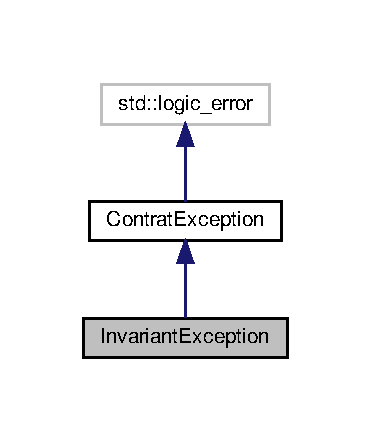
\includegraphics[width=178pt]{classInvariantException__inherit__graph}
\end{center}
\end{figure}


Collaboration diagram for Invariant\+Exception\+:\nopagebreak
\begin{figure}[H]
\begin{center}
\leavevmode
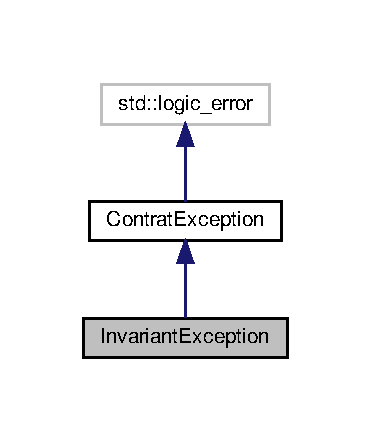
\includegraphics[width=178pt]{classInvariantException__coll__graph}
\end{center}
\end{figure}
\subsection*{Public Member Functions}
\begin{DoxyCompactItemize}
\item 
\hyperlink{classInvariantException_af8a1950834b26c256db0b11eb33e6056}{Invariant\+Exception} (std\+::string, unsigned int, std\+::string)
\begin{DoxyCompactList}\small\item\em Constructeur de la classe \hyperlink{classInvariantException}{Invariant\+Exception} en initialisant la classe de base \hyperlink{classContratException}{Contrat\+Exception}. La classe représente des erreurs d\textquotesingle{}invariant dans la théorie du contrat. \end{DoxyCompactList}\end{DoxyCompactItemize}


\subsection{Detailed Description}
Classe pour la gestion des erreurs d\textquotesingle{}invariant. 

\subsection{Constructor \& Destructor Documentation}
\mbox{\Hypertarget{classInvariantException_af8a1950834b26c256db0b11eb33e6056}\label{classInvariantException_af8a1950834b26c256db0b11eb33e6056}} 
\index{Invariant\+Exception@{Invariant\+Exception}!Invariant\+Exception@{Invariant\+Exception}}
\index{Invariant\+Exception@{Invariant\+Exception}!Invariant\+Exception@{Invariant\+Exception}}
\subsubsection{\texorpdfstring{Invariant\+Exception()}{InvariantException()}}
{\footnotesize\ttfamily Invariant\+Exception\+::\+Invariant\+Exception (\begin{DoxyParamCaption}\item[{std\+::string}]{p\+\_\+fichP,  }\item[{unsigned int}]{p\+\_\+prm\+Ligne,  }\item[{std\+::string}]{p\+\_\+exprP }\end{DoxyParamCaption})}



Constructeur de la classe \hyperlink{classInvariantException}{Invariant\+Exception} en initialisant la classe de base \hyperlink{classContratException}{Contrat\+Exception}. La classe représente des erreurs d\textquotesingle{}invariant dans la théorie du contrat. 


\begin{DoxyParams}{Parameters}
{\em p\+\_\+fichP} & chaîne de caractères représentant le fichier source dans lequel a eu lieu l\textquotesingle{}erreur \\
\hline
{\em p\+\_\+prm\+Ligne} & un entier représentant la ligne où a eu lieu l\textquotesingle{}erreur \\
\hline
{\em p\+\_\+exprP} & Test logique qui a échoué \\
\hline
\end{DoxyParams}


The documentation for this class was generated from the following files\+:\begin{DoxyCompactItemize}
\item 
\hyperlink{ContratException_8h}{Contrat\+Exception.\+h}\item 
\hyperlink{ContratException_8cpp}{Contrat\+Exception.\+cpp}\end{DoxyCompactItemize}

\hypertarget{classhockey_1_1Joueur}{}\section{hockey\+:\+:Joueur Class Reference}
\label{classhockey_1_1Joueur}\index{hockey\+::\+Joueur@{hockey\+::\+Joueur}}


Cette classe sert au maintien et à la manipulation des joueurs. Elle hérite de la classe \hyperlink{classhockey_1_1Personne}{Personne}.  




{\ttfamily \#include $<$Joueur.\+h$>$}



Inheritance diagram for hockey\+:\+:Joueur\+:\nopagebreak
\begin{figure}[H]
\begin{center}
\leavevmode
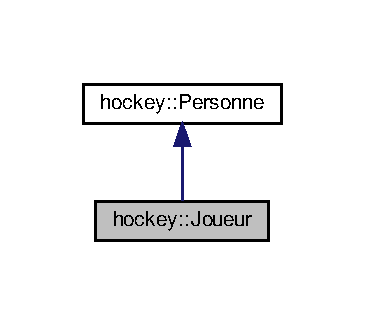
\includegraphics[width=175pt]{classhockey_1_1Joueur__inherit__graph}
\end{center}
\end{figure}


Collaboration diagram for hockey\+:\+:Joueur\+:\nopagebreak
\begin{figure}[H]
\begin{center}
\leavevmode
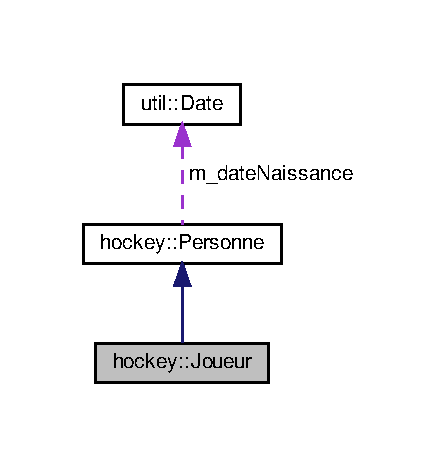
\includegraphics[width=209pt]{classhockey_1_1Joueur__coll__graph}
\end{center}
\end{figure}
\subsection*{Public Member Functions}
\begin{DoxyCompactItemize}
\item 
\hyperlink{classhockey_1_1Joueur_a07cc484db0a5b94fb425aff475c123e2}{Joueur} (std\+::string p\+\_\+nom, std\+::string p\+\_\+prenom, const \hyperlink{classutil_1_1Date}{util\+::\+Date} \&p\+\_\+date\+Naissance, std\+::string p\+\_\+telephone, std\+::string p\+\_\+position)
\begin{DoxyCompactList}\small\item\em Constructeur de la classe \hyperlink{classhockey_1_1Joueur}{Joueur} avec des paramètres en entrée. \end{DoxyCompactList}\item 
\mbox{\Hypertarget{classhockey_1_1Joueur_a822dae0ca7b05d7637eab533656dfe22}\label{classhockey_1_1Joueur_a822dae0ca7b05d7637eab533656dfe22}} 
\hyperlink{classhockey_1_1Joueur_a822dae0ca7b05d7637eab533656dfe22}{Joueur} ()
\begin{DoxyCompactList}\small\item\em Constructeur par défaut sans paramètres. Permet de retourner une erreur de précondition s\textquotesingle{}il est utilisé. \end{DoxyCompactList}\item 
const std\+::string \& \hyperlink{classhockey_1_1Joueur_a7c9bc7262096861271b4e0431dcd1693}{req\+Position} () const
\begin{DoxyCompactList}\small\item\em Méthode permettant de retourner la position du joueur. \end{DoxyCompactList}\item 
virtual std\+::string \hyperlink{classhockey_1_1Joueur_ab3d6b15e55aa765807e4960108f7db29}{req\+Personne\+Formate} () const
\begin{DoxyCompactList}\small\item\em Méthode permettant de retourner les informations du joueur. \end{DoxyCompactList}\item 
virtual \hyperlink{classhockey_1_1Personne}{Personne} $\ast$ \hyperlink{classhockey_1_1Joueur_a29a2fc040b74bf3bf72d7670012c9bff}{clone} () const
\begin{DoxyCompactList}\small\item\em Méthode permettant de créer une nouvelle instance du joueur. \end{DoxyCompactList}\item 
\mbox{\Hypertarget{classhockey_1_1Joueur_a3f385cd26133b8fe8c2afce4c70c9ece}\label{classhockey_1_1Joueur_a3f385cd26133b8fe8c2afce4c70c9ece}} 
virtual \hyperlink{classhockey_1_1Joueur_a3f385cd26133b8fe8c2afce4c70c9ece}{$\sim$\+Joueur} ()
\begin{DoxyCompactList}\small\item\em Destructeur de la classe \hyperlink{classhockey_1_1Joueur}{Joueur}. \end{DoxyCompactList}\end{DoxyCompactItemize}
\subsection*{Additional Inherited Members}


\subsection{Detailed Description}
Cette classe sert au maintien et à la manipulation des joueurs. Elle hérite de la classe \hyperlink{classhockey_1_1Personne}{Personne}. 

Les valeurs qui entrent dans la classe doivent être validée à priori. 

Attributs\+: string p\+\_\+nom, string p\+\_\+prenom, Date p\+\_\+date\+Naissance, string p\+\_\+telephone, string p\+\_\+position 

\subsection{Constructor \& Destructor Documentation}
\mbox{\Hypertarget{classhockey_1_1Joueur_a07cc484db0a5b94fb425aff475c123e2}\label{classhockey_1_1Joueur_a07cc484db0a5b94fb425aff475c123e2}} 
\index{hockey\+::\+Joueur@{hockey\+::\+Joueur}!Joueur@{Joueur}}
\index{Joueur@{Joueur}!hockey\+::\+Joueur@{hockey\+::\+Joueur}}
\subsubsection{\texorpdfstring{Joueur()}{Joueur()}}
{\footnotesize\ttfamily hockey\+::\+Joueur\+::\+Joueur (\begin{DoxyParamCaption}\item[{std\+::string}]{p\+\_\+nom,  }\item[{std\+::string}]{p\+\_\+prenom,  }\item[{const \hyperlink{classutil_1_1Date}{util\+::\+Date} \&}]{p\+\_\+date\+Naissance,  }\item[{std\+::string}]{p\+\_\+telephone,  }\item[{std\+::string}]{p\+\_\+position }\end{DoxyParamCaption})}



Constructeur de la classe \hyperlink{classhockey_1_1Joueur}{Joueur} avec des paramètres en entrée. 


\begin{DoxyParams}[1]{Parameters}
\mbox{\tt in}  & {\em p\+\_\+nom} & un string représentant le nom du joueur \\
\hline
\mbox{\tt in}  & {\em p\+\_\+prenom} & un string représentant le prénom du joueur \\
\hline
\mbox{\tt in}  & {\em p\+\_\+date\+Naissance} & un objet Date représentant la date de naissance du joueur \\
\hline
\mbox{\tt in}  & {\em p\+\_\+telephone} & un string représentant le numéro de téléphone du joueur \\
\hline
\mbox{\tt in}  & {\em p\+\_\+position} & \\
\hline
\end{DoxyParams}
\begin{DoxyPrecond}{Precondition}
Tous les paramètres en entrée doivent être valide pour une personne standard. 

La position du joueur doit être \char`\"{}centre\char`\"{},\char`\"{}ailier\char`\"{},\char`\"{}gardien\char`\"{} ou \char`\"{}défenseur\char`\"{} 
\end{DoxyPrecond}
\begin{DoxyInvariant}{Invariant}
Les invariants d\textquotesingle{}un joueur sont les mêmes que ceux d\textquotesingle{}une personne standard. 

Le joueur doit avoir une position valide. 
\end{DoxyInvariant}


\subsection{Member Function Documentation}
\mbox{\Hypertarget{classhockey_1_1Joueur_a29a2fc040b74bf3bf72d7670012c9bff}\label{classhockey_1_1Joueur_a29a2fc040b74bf3bf72d7670012c9bff}} 
\index{hockey\+::\+Joueur@{hockey\+::\+Joueur}!clone@{clone}}
\index{clone@{clone}!hockey\+::\+Joueur@{hockey\+::\+Joueur}}
\subsubsection{\texorpdfstring{clone()}{clone()}}
{\footnotesize\ttfamily \hyperlink{classhockey_1_1Personne}{Personne} $\ast$ hockey\+::\+Joueur\+::clone (\begin{DoxyParamCaption}{ }\end{DoxyParamCaption}) const\hspace{0.3cm}{\ttfamily [virtual]}}



Méthode permettant de créer une nouvelle instance du joueur. 

\begin{DoxyReturn}{Returns}
un pointeur vers la nouvelle instance du joueur. 
\end{DoxyReturn}


Implements \hyperlink{classhockey_1_1Personne}{hockey\+::\+Personne}.

\mbox{\Hypertarget{classhockey_1_1Joueur_ab3d6b15e55aa765807e4960108f7db29}\label{classhockey_1_1Joueur_ab3d6b15e55aa765807e4960108f7db29}} 
\index{hockey\+::\+Joueur@{hockey\+::\+Joueur}!req\+Personne\+Formate@{req\+Personne\+Formate}}
\index{req\+Personne\+Formate@{req\+Personne\+Formate}!hockey\+::\+Joueur@{hockey\+::\+Joueur}}
\subsubsection{\texorpdfstring{req\+Personne\+Formate()}{reqPersonneFormate()}}
{\footnotesize\ttfamily string hockey\+::\+Joueur\+::req\+Personne\+Formate (\begin{DoxyParamCaption}{ }\end{DoxyParamCaption}) const\hspace{0.3cm}{\ttfamily [virtual]}}



Méthode permettant de retourner les informations du joueur. 

\begin{DoxyReturn}{Returns}
un string représentant les informations du joueur 
\end{DoxyReturn}


Reimplemented from \hyperlink{classhockey_1_1Personne_ae67b3d253c1fa8a090dd8040ca1e8ccc}{hockey\+::\+Personne}.

\mbox{\Hypertarget{classhockey_1_1Joueur_a7c9bc7262096861271b4e0431dcd1693}\label{classhockey_1_1Joueur_a7c9bc7262096861271b4e0431dcd1693}} 
\index{hockey\+::\+Joueur@{hockey\+::\+Joueur}!req\+Position@{req\+Position}}
\index{req\+Position@{req\+Position}!hockey\+::\+Joueur@{hockey\+::\+Joueur}}
\subsubsection{\texorpdfstring{req\+Position()}{reqPosition()}}
{\footnotesize\ttfamily const string \& hockey\+::\+Joueur\+::req\+Position (\begin{DoxyParamCaption}{ }\end{DoxyParamCaption}) const}



Méthode permettant de retourner la position du joueur. 

\begin{DoxyReturn}{Returns}
un string représentant la position du joueur 
\end{DoxyReturn}


The documentation for this class was generated from the following files\+:\begin{DoxyCompactItemize}
\item 
\hyperlink{Joueur_8h}{Joueur.\+h}\item 
\hyperlink{Joueur_8cpp}{Joueur.\+cpp}\end{DoxyCompactItemize}

\hypertarget{classhockey_1_1Personne}{}\section{hockey\+:\+:Personne Class Reference}
\label{classhockey_1_1Personne}\index{hockey\+::\+Personne@{hockey\+::\+Personne}}


Cette classe sert au maintien et à la manipulation des personnes.  




{\ttfamily \#include $<$Personne.\+h$>$}



Inheritance diagram for hockey\+:\+:Personne\+:\nopagebreak
\begin{figure}[H]
\begin{center}
\leavevmode
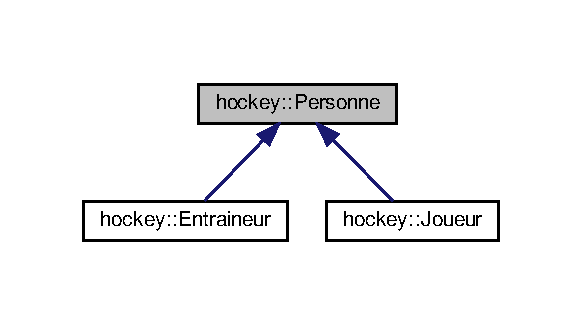
\includegraphics[width=279pt]{classhockey_1_1Personne__inherit__graph}
\end{center}
\end{figure}


Collaboration diagram for hockey\+:\+:Personne\+:\nopagebreak
\begin{figure}[H]
\begin{center}
\leavevmode
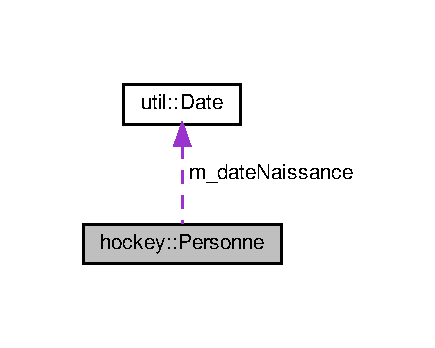
\includegraphics[width=209pt]{classhockey_1_1Personne__coll__graph}
\end{center}
\end{figure}
\subsection*{Public Member Functions}
\begin{DoxyCompactItemize}
\item 
\mbox{\Hypertarget{classhockey_1_1Personne_ad712e93d7629f8cab38821139d9dc2af}\label{classhockey_1_1Personne_ad712e93d7629f8cab38821139d9dc2af}} 
\hyperlink{classhockey_1_1Personne_ad712e93d7629f8cab38821139d9dc2af}{Personne} ()
\begin{DoxyCompactList}\small\item\em constructeur d\textquotesingle{}un objet \hyperlink{classhockey_1_1Personne}{Personne} vide. Ce constructeur existe pour renvoyer une erreur si un objet \hyperlink{classhockey_1_1Personne}{Personne} est créé sans paramètres \end{DoxyCompactList}\item 
\hyperlink{classhockey_1_1Personne_ab38273cfbd7a665a10b20b5d44255482}{Personne} (std\+::string p\+\_\+nom, std\+::string p\+\_\+prenom, const \hyperlink{classutil_1_1Date}{util\+::\+Date} \&p\+\_\+date\+Naissance, std\+::string p\+\_\+telephone)
\begin{DoxyCompactList}\small\item\em constructeur d\textquotesingle{}un objet \hyperlink{classhockey_1_1Personne}{Personne} à partir de valeurs passées en paramètres. \end{DoxyCompactList}\item 
const \hyperlink{classutil_1_1Date}{util\+::\+Date} \hyperlink{classhockey_1_1Personne_ae9cb2402f8012b71959846a079986308}{req\+Date\+Naissance} () const
\begin{DoxyCompactList}\small\item\em retourne la date de naissance de la personne . \end{DoxyCompactList}\item 
const std\+::string \& \hyperlink{classhockey_1_1Personne_a0fdf8d98c481d17234c995bf67b57091}{req\+Nom} () const
\begin{DoxyCompactList}\small\item\em retourne le nom de le personne. \end{DoxyCompactList}\item 
const std\+::string \& \hyperlink{classhockey_1_1Personne_ae4257bc9fcd9f97d2a982797642401ee}{req\+Prenom} () const
\begin{DoxyCompactList}\small\item\em retourne le prénom de le personne. \end{DoxyCompactList}\item 
const std\+::string \& \hyperlink{classhockey_1_1Personne_ad6b6a4dc6bb847c2bec38acb9104e378}{req\+Telephone} () const
\begin{DoxyCompactList}\small\item\em retourne le téléphone de le personne. \end{DoxyCompactList}\item 
void \hyperlink{classhockey_1_1Personne_a82838fb8c45d908b64396e14787f4d52}{asg\+Telephone} (const std\+::string \&p\+\_\+telephone)
\begin{DoxyCompactList}\small\item\em asigne un nouveau numéro de téléphone à la personne. \end{DoxyCompactList}\item 
virtual std\+::string \hyperlink{classhockey_1_1Personne_ae67b3d253c1fa8a090dd8040ca1e8ccc}{req\+Personne\+Formate} () const
\begin{DoxyCompactList}\small\item\em créer une chaîne de caractères (string) représentant les informations de la personne. \end{DoxyCompactList}\item 
bool \hyperlink{classhockey_1_1Personne_a5a519977d574d18b919eb39e6cfbf62b}{operator==} (const \hyperlink{classhockey_1_1Personne}{Personne} \&p\+\_\+personne) const
\begin{DoxyCompactList}\small\item\em surcharge de l\textquotesingle{}opérateur == pour les objets \hyperlink{classhockey_1_1Personne}{Personne}. \end{DoxyCompactList}\item 
\mbox{\Hypertarget{classhockey_1_1Personne_a4e81e9f921891b0bd1b3bbe859d3fae0}\label{classhockey_1_1Personne_a4e81e9f921891b0bd1b3bbe859d3fae0}} 
virtual \hyperlink{classhockey_1_1Personne}{Personne} $\ast$ {\bfseries clone} () const =0
\end{DoxyCompactItemize}
\subsection*{Protected Attributes}
\begin{DoxyCompactItemize}
\item 
\mbox{\Hypertarget{classhockey_1_1Personne_a77d1c72b30b7cfad33714688d665ff05}\label{classhockey_1_1Personne_a77d1c72b30b7cfad33714688d665ff05}} 
\hyperlink{classutil_1_1Date}{util\+::\+Date} {\bfseries m\+\_\+date\+Naissance}
\end{DoxyCompactItemize}


\subsection{Detailed Description}
Cette classe sert au maintien et à la manipulation des personnes. 

Cette classe est abstraite. 

Les valeurs qui entrent dans la classe doivent être validée à priori. 

Attributs\+: string p\+\_\+nom, string p\+\_\+prenom, Date p\+\_\+date\+Naissance, string p\+\_\+telephone 

\subsection{Constructor \& Destructor Documentation}
\mbox{\Hypertarget{classhockey_1_1Personne_ab38273cfbd7a665a10b20b5d44255482}\label{classhockey_1_1Personne_ab38273cfbd7a665a10b20b5d44255482}} 
\index{hockey\+::\+Personne@{hockey\+::\+Personne}!Personne@{Personne}}
\index{Personne@{Personne}!hockey\+::\+Personne@{hockey\+::\+Personne}}
\subsubsection{\texorpdfstring{Personne()}{Personne()}}
{\footnotesize\ttfamily hockey\+::\+Personne\+::\+Personne (\begin{DoxyParamCaption}\item[{std\+::string}]{p\+\_\+nom,  }\item[{std\+::string}]{p\+\_\+prenom,  }\item[{const \hyperlink{classutil_1_1Date}{util\+::\+Date} \&}]{p\+\_\+date\+Naissance,  }\item[{std\+::string}]{p\+\_\+telephone }\end{DoxyParamCaption})}



constructeur d\textquotesingle{}un objet \hyperlink{classhockey_1_1Personne}{Personne} à partir de valeurs passées en paramètres. 


\begin{DoxyParams}[1]{Parameters}
\mbox{\tt in}  & {\em p\+\_\+nom} & est une chaîne de caractères (string) qui représente le nom de la personne créée. \\
\hline
\mbox{\tt in}  & {\em p\+\_\+prenom} & est une chaîne de caractères (string) qui représente le prénom de la personne créée. \\
\hline
\mbox{\tt in}  & {\em p\+\_\+date\+Naissance} & est un objet Date qui représente la date de naissance de la personne créée. \\
\hline
\mbox{\tt in}  & {\em p\+\_\+telephone} & est une chaîne de caractères (string) qui représente le prénom de la personne créée. \\
\hline
\end{DoxyParams}
\begin{DoxyPrecond}{Precondition}
Les valeurs entrées doivent être valides et avoir un format valide. 
\end{DoxyPrecond}


\subsection{Member Function Documentation}
\mbox{\Hypertarget{classhockey_1_1Personne_a82838fb8c45d908b64396e14787f4d52}\label{classhockey_1_1Personne_a82838fb8c45d908b64396e14787f4d52}} 
\index{hockey\+::\+Personne@{hockey\+::\+Personne}!asg\+Telephone@{asg\+Telephone}}
\index{asg\+Telephone@{asg\+Telephone}!hockey\+::\+Personne@{hockey\+::\+Personne}}
\subsubsection{\texorpdfstring{asg\+Telephone()}{asgTelephone()}}
{\footnotesize\ttfamily void hockey\+::\+Personne\+::asg\+Telephone (\begin{DoxyParamCaption}\item[{const std\+::string \&}]{p\+\_\+telephone }\end{DoxyParamCaption})}



asigne un nouveau numéro de téléphone à la personne. 


\begin{DoxyParams}[1]{Parameters}
\mbox{\tt in}  & {\em p\+\_\+telephone} & une chaîne de caractère (string) qui représente le numéro de téléphone de la personne. \\
\hline
\end{DoxyParams}
\begin{DoxyPrecond}{Precondition}
le numéro de téléphone doit être valide et dans un format valide X\+XX X\+X\+X-\/\+X\+X\+XX. 
\end{DoxyPrecond}
\mbox{\Hypertarget{classhockey_1_1Personne_a5a519977d574d18b919eb39e6cfbf62b}\label{classhockey_1_1Personne_a5a519977d574d18b919eb39e6cfbf62b}} 
\index{hockey\+::\+Personne@{hockey\+::\+Personne}!operator==@{operator==}}
\index{operator==@{operator==}!hockey\+::\+Personne@{hockey\+::\+Personne}}
\subsubsection{\texorpdfstring{operator==()}{operator==()}}
{\footnotesize\ttfamily bool hockey\+::\+Personne\+::operator== (\begin{DoxyParamCaption}\item[{const \hyperlink{classhockey_1_1Personne}{Personne} \&}]{p\+\_\+personne }\end{DoxyParamCaption}) const}



surcharge de l\textquotesingle{}opérateur == pour les objets \hyperlink{classhockey_1_1Personne}{Personne}. 


\begin{DoxyParams}[1]{Parameters}
\mbox{\tt in}  & {\em p\+\_\+personne} & qui est une personne valide. \\
\hline
\end{DoxyParams}
\begin{DoxyReturn}{Returns}
un booléen indiquant si les deux personnes sont égales ou pas sur la base de leur nom, prénom et date de naissance. 
\end{DoxyReturn}
\mbox{\Hypertarget{classhockey_1_1Personne_ae9cb2402f8012b71959846a079986308}\label{classhockey_1_1Personne_ae9cb2402f8012b71959846a079986308}} 
\index{hockey\+::\+Personne@{hockey\+::\+Personne}!req\+Date\+Naissance@{req\+Date\+Naissance}}
\index{req\+Date\+Naissance@{req\+Date\+Naissance}!hockey\+::\+Personne@{hockey\+::\+Personne}}
\subsubsection{\texorpdfstring{req\+Date\+Naissance()}{reqDateNaissance()}}
{\footnotesize\ttfamily const \hyperlink{classutil_1_1Date}{util\+::\+Date} hockey\+::\+Personne\+::req\+Date\+Naissance (\begin{DoxyParamCaption}{ }\end{DoxyParamCaption}) const}



retourne la date de naissance de la personne . 

\begin{DoxyReturn}{Returns}
un objet date qui représente la date de naissance de la personne. 
\end{DoxyReturn}
\mbox{\Hypertarget{classhockey_1_1Personne_a0fdf8d98c481d17234c995bf67b57091}\label{classhockey_1_1Personne_a0fdf8d98c481d17234c995bf67b57091}} 
\index{hockey\+::\+Personne@{hockey\+::\+Personne}!req\+Nom@{req\+Nom}}
\index{req\+Nom@{req\+Nom}!hockey\+::\+Personne@{hockey\+::\+Personne}}
\subsubsection{\texorpdfstring{req\+Nom()}{reqNom()}}
{\footnotesize\ttfamily const string \& hockey\+::\+Personne\+::req\+Nom (\begin{DoxyParamCaption}{ }\end{DoxyParamCaption}) const}



retourne le nom de le personne. 

\begin{DoxyReturn}{Returns}
une chaîne de caractères (string) qui représente le nom de la personne. 
\end{DoxyReturn}
\mbox{\Hypertarget{classhockey_1_1Personne_ae67b3d253c1fa8a090dd8040ca1e8ccc}\label{classhockey_1_1Personne_ae67b3d253c1fa8a090dd8040ca1e8ccc}} 
\index{hockey\+::\+Personne@{hockey\+::\+Personne}!req\+Personne\+Formate@{req\+Personne\+Formate}}
\index{req\+Personne\+Formate@{req\+Personne\+Formate}!hockey\+::\+Personne@{hockey\+::\+Personne}}
\subsubsection{\texorpdfstring{req\+Personne\+Formate()}{reqPersonneFormate()}}
{\footnotesize\ttfamily string hockey\+::\+Personne\+::req\+Personne\+Formate (\begin{DoxyParamCaption}{ }\end{DoxyParamCaption}) const\hspace{0.3cm}{\ttfamily [virtual]}}



créer une chaîne de caractères (string) représentant les informations de la personne. 

\begin{DoxyReturn}{Returns}
une chaîne de caractères (string) représentant les informations de la personne. 
\end{DoxyReturn}


Reimplemented in \hyperlink{classhockey_1_1Entraineur_a376149c10b8541c45d703682d41d80f3}{hockey\+::\+Entraineur}, and \hyperlink{classhockey_1_1Joueur_ab3d6b15e55aa765807e4960108f7db29}{hockey\+::\+Joueur}.

\mbox{\Hypertarget{classhockey_1_1Personne_ae4257bc9fcd9f97d2a982797642401ee}\label{classhockey_1_1Personne_ae4257bc9fcd9f97d2a982797642401ee}} 
\index{hockey\+::\+Personne@{hockey\+::\+Personne}!req\+Prenom@{req\+Prenom}}
\index{req\+Prenom@{req\+Prenom}!hockey\+::\+Personne@{hockey\+::\+Personne}}
\subsubsection{\texorpdfstring{req\+Prenom()}{reqPrenom()}}
{\footnotesize\ttfamily const string \& hockey\+::\+Personne\+::req\+Prenom (\begin{DoxyParamCaption}{ }\end{DoxyParamCaption}) const}



retourne le prénom de le personne. 

\begin{DoxyReturn}{Returns}
une chaîne de caractères (string) qui représente le prénom de la personne. 
\end{DoxyReturn}
\mbox{\Hypertarget{classhockey_1_1Personne_ad6b6a4dc6bb847c2bec38acb9104e378}\label{classhockey_1_1Personne_ad6b6a4dc6bb847c2bec38acb9104e378}} 
\index{hockey\+::\+Personne@{hockey\+::\+Personne}!req\+Telephone@{req\+Telephone}}
\index{req\+Telephone@{req\+Telephone}!hockey\+::\+Personne@{hockey\+::\+Personne}}
\subsubsection{\texorpdfstring{req\+Telephone()}{reqTelephone()}}
{\footnotesize\ttfamily const string \& hockey\+::\+Personne\+::req\+Telephone (\begin{DoxyParamCaption}{ }\end{DoxyParamCaption}) const}



retourne le téléphone de le personne. 

\begin{DoxyReturn}{Returns}
une chaîne de caractères (string) qui représente le numéro de téléphone de la personne. 
\end{DoxyReturn}


The documentation for this class was generated from the following files\+:\begin{DoxyCompactItemize}
\item 
\hyperlink{Personne_8h}{Personne.\+h}\item 
\hyperlink{Personne_8cpp}{Personne.\+cpp}\end{DoxyCompactItemize}

\hypertarget{classPostconditionException}{}\section{Postcondition\+Exception Class Reference}
\label{classPostconditionException}\index{Postcondition\+Exception@{Postcondition\+Exception}}


Classe pour la gestion des erreurs de postcondition.  




{\ttfamily \#include $<$Contrat\+Exception.\+h$>$}



Inheritance diagram for Postcondition\+Exception\+:\nopagebreak
\begin{figure}[H]
\begin{center}
\leavevmode
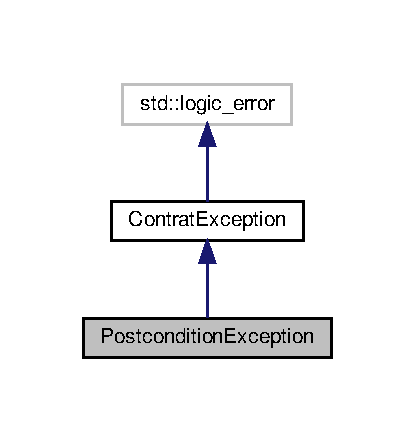
\includegraphics[width=199pt]{classPostconditionException__inherit__graph}
\end{center}
\end{figure}


Collaboration diagram for Postcondition\+Exception\+:\nopagebreak
\begin{figure}[H]
\begin{center}
\leavevmode
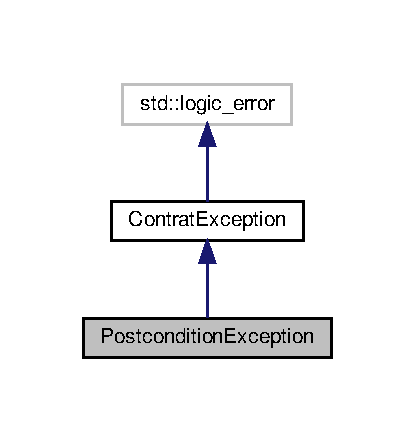
\includegraphics[width=199pt]{classPostconditionException__coll__graph}
\end{center}
\end{figure}
\subsection*{Public Member Functions}
\begin{DoxyCompactItemize}
\item 
\hyperlink{classPostconditionException_acc95ea17c4302b996261b7201d2cf6c4}{Postcondition\+Exception} (std\+::string, unsigned int, std\+::string)
\begin{DoxyCompactList}\small\item\em Constructeur de la classe \hyperlink{classPostconditionException}{Postcondition\+Exception} en initialisant la classe de base \hyperlink{classContratException}{Contrat\+Exception}. La classe représente des erreurs de postcondition dans la théorie du contrat. \end{DoxyCompactList}\end{DoxyCompactItemize}


\subsection{Detailed Description}
Classe pour la gestion des erreurs de postcondition. 

\subsection{Constructor \& Destructor Documentation}
\mbox{\Hypertarget{classPostconditionException_acc95ea17c4302b996261b7201d2cf6c4}\label{classPostconditionException_acc95ea17c4302b996261b7201d2cf6c4}} 
\index{Postcondition\+Exception@{Postcondition\+Exception}!Postcondition\+Exception@{Postcondition\+Exception}}
\index{Postcondition\+Exception@{Postcondition\+Exception}!Postcondition\+Exception@{Postcondition\+Exception}}
\subsubsection{\texorpdfstring{Postcondition\+Exception()}{PostconditionException()}}
{\footnotesize\ttfamily Postcondition\+Exception\+::\+Postcondition\+Exception (\begin{DoxyParamCaption}\item[{std\+::string}]{p\+\_\+fichP,  }\item[{unsigned int}]{p\+\_\+prm\+Ligne,  }\item[{std\+::string}]{p\+\_\+exprP }\end{DoxyParamCaption})}



Constructeur de la classe \hyperlink{classPostconditionException}{Postcondition\+Exception} en initialisant la classe de base \hyperlink{classContratException}{Contrat\+Exception}. La classe représente des erreurs de postcondition dans la théorie du contrat. 


\begin{DoxyParams}{Parameters}
{\em p\+\_\+fichP} & chaîne de caractères représentant le fichier source dans lequel a eu lieu l\textquotesingle{}erreur \\
\hline
{\em p\+\_\+prm\+Ligne} & un entier représentant la ligne où a eu lieu l\textquotesingle{}erreur \\
\hline
{\em p\+\_\+exprP} & Test logique qui a échoué \\
\hline
\end{DoxyParams}


The documentation for this class was generated from the following files\+:\begin{DoxyCompactItemize}
\item 
\hyperlink{ContratException_8h}{Contrat\+Exception.\+h}\item 
\hyperlink{ContratException_8cpp}{Contrat\+Exception.\+cpp}\end{DoxyCompactItemize}

\hypertarget{classPreconditionException}{}\section{Precondition\+Exception Class Reference}
\label{classPreconditionException}\index{Precondition\+Exception@{Precondition\+Exception}}


Classe pour la gestion des erreurs de précondition.  




{\ttfamily \#include $<$Contrat\+Exception.\+h$>$}



Inheritance diagram for Precondition\+Exception\+:\nopagebreak
\begin{figure}[H]
\begin{center}
\leavevmode
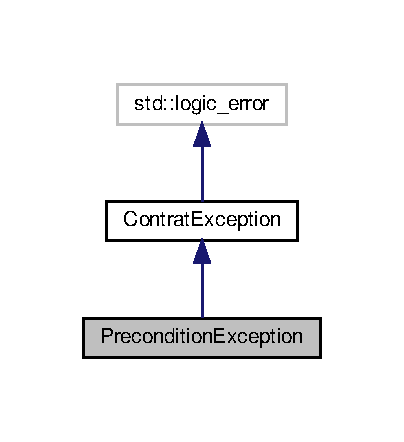
\includegraphics[width=194pt]{classPreconditionException__inherit__graph}
\end{center}
\end{figure}


Collaboration diagram for Precondition\+Exception\+:\nopagebreak
\begin{figure}[H]
\begin{center}
\leavevmode
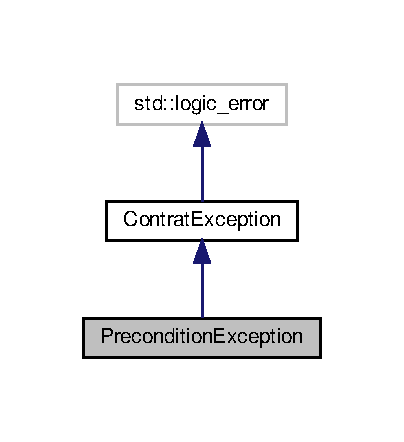
\includegraphics[width=194pt]{classPreconditionException__coll__graph}
\end{center}
\end{figure}
\subsection*{Public Member Functions}
\begin{DoxyCompactItemize}
\item 
\hyperlink{classPreconditionException_a66d4b4c57a0675d487dab85d2c31b08c}{Precondition\+Exception} (std\+::string, unsigned int, std\+::string)
\begin{DoxyCompactList}\small\item\em Constructeur de la classe \hyperlink{classPreconditionException}{Precondition\+Exception} en initialisant la classe de base \hyperlink{classContratException}{Contrat\+Exception}. La classe représente l\textquotesingle{}erreur de précondition dans la théorie du contrat. \end{DoxyCompactList}\end{DoxyCompactItemize}


\subsection{Detailed Description}
Classe pour la gestion des erreurs de précondition. 

\subsection{Constructor \& Destructor Documentation}
\mbox{\Hypertarget{classPreconditionException_a66d4b4c57a0675d487dab85d2c31b08c}\label{classPreconditionException_a66d4b4c57a0675d487dab85d2c31b08c}} 
\index{Precondition\+Exception@{Precondition\+Exception}!Precondition\+Exception@{Precondition\+Exception}}
\index{Precondition\+Exception@{Precondition\+Exception}!Precondition\+Exception@{Precondition\+Exception}}
\subsubsection{\texorpdfstring{Precondition\+Exception()}{PreconditionException()}}
{\footnotesize\ttfamily Precondition\+Exception\+::\+Precondition\+Exception (\begin{DoxyParamCaption}\item[{std\+::string}]{p\+\_\+fichP,  }\item[{unsigned int}]{p\+\_\+prm\+Ligne,  }\item[{std\+::string}]{p\+\_\+exprP }\end{DoxyParamCaption})}



Constructeur de la classe \hyperlink{classPreconditionException}{Precondition\+Exception} en initialisant la classe de base \hyperlink{classContratException}{Contrat\+Exception}. La classe représente l\textquotesingle{}erreur de précondition dans la théorie du contrat. 


\begin{DoxyParams}{Parameters}
{\em p\+\_\+fichP} & chaîne de caractères représentant le fichier source dans lequel a eu lieu l\textquotesingle{}erreur \\
\hline
{\em p\+\_\+prm\+Ligne} & un entier représentant la ligne où a eu lieu l\textquotesingle{}erreur \\
\hline
{\em p\+\_\+exprP} & Test logique qui a échoué \\
\hline
\end{DoxyParams}


The documentation for this class was generated from the following files\+:\begin{DoxyCompactItemize}
\item 
\hyperlink{ContratException_8h}{Contrat\+Exception.\+h}\item 
\hyperlink{ContratException_8cpp}{Contrat\+Exception.\+cpp}\end{DoxyCompactItemize}

\chapter{File Documentation}
\hypertarget{Annuaire_8cpp}{}\section{Annuaire.\+cpp File Reference}
\label{Annuaire_8cpp}\index{Annuaire.\+cpp@{Annuaire.\+cpp}}


Fichier qui contient l\textquotesingle{}implémentation de la classe Annuaire. Cette classe permet de gérer les différentes personnes membre d\textquotesingle{}une équipe de hockey.  


{\ttfamily \#include $<$sstream$>$}\newline
{\ttfamily \#include $<$iomanip$>$}\newline
{\ttfamily \#include \char`\"{}Contrat\+Exception.\+h\char`\"{}}\newline
{\ttfamily \#include \char`\"{}Annuaire.\+h\char`\"{}}\newline
Include dependency graph for Annuaire.\+cpp\+:\nopagebreak
\begin{figure}[H]
\begin{center}
\leavevmode
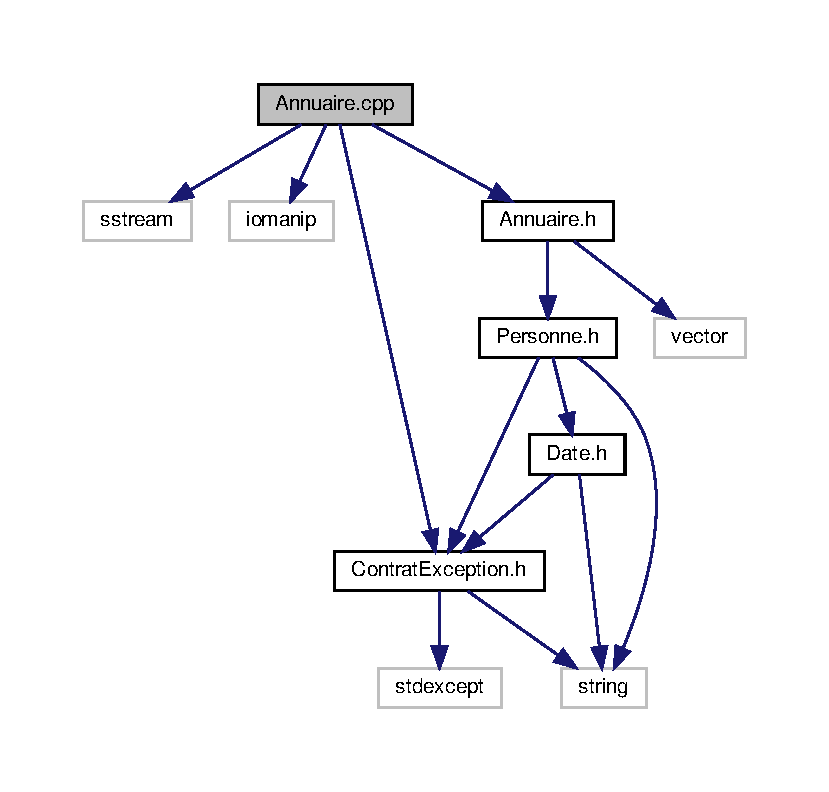
\includegraphics[width=350pt]{Annuaire_8cpp__incl}
\end{center}
\end{figure}


\subsection{Detailed Description}
Fichier qui contient l\textquotesingle{}implémentation de la classe Annuaire. Cette classe permet de gérer les différentes personnes membre d\textquotesingle{}une équipe de hockey. 

Attributs\+:
\begin{DoxyItemize}
\item string m\+\_\+nom\+Club\+: Le nom de l\textquotesingle{}équipe de hockey.
\item vector$<$$\ast$\+Personne$>$ m\+\_\+v\+Membres\+: un vecteur contenant des pointeurs vers les personnes membres de l\textquotesingle{}équipe ajouter à l\textquotesingle{}Annuaire. \begin{DoxyAuthor}{Author}
Jordan Longval 
\end{DoxyAuthor}
\begin{DoxyVersion}{Version}
T\+P3 
\end{DoxyVersion}
\begin{DoxyDate}{Date}
\+: 2020-\/04-\/02 
\end{DoxyDate}

\end{DoxyItemize}
\hypertarget{Annuaire_8h}{}\section{Annuaire.\+h File Reference}
\label{Annuaire_8h}\index{Annuaire.\+h@{Annuaire.\+h}}


\+: Fichier qui contient l\textquotesingle{}interface de la classe annuaire qui permet de faire la gestion des personnes membres d\textquotesingle{}une équipe de hockey dans un annuaire.  


{\ttfamily \#include $<$vector$>$}\newline
{\ttfamily \#include \char`\"{}Personne.\+h\char`\"{}}\newline
Include dependency graph for Annuaire.\+h\+:\nopagebreak
\begin{figure}[H]
\begin{center}
\leavevmode
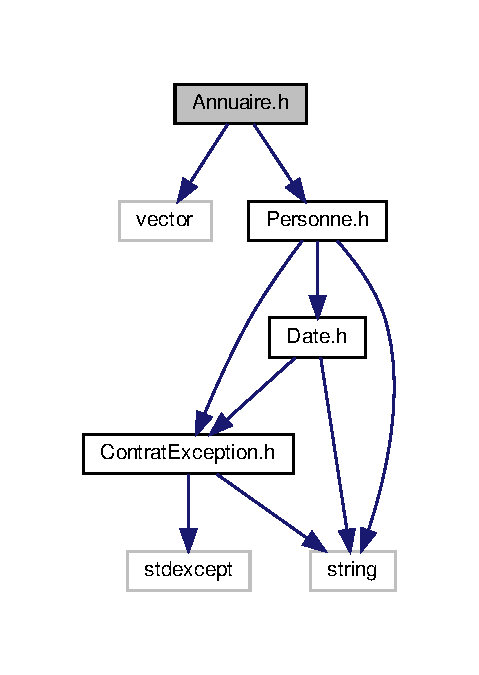
\includegraphics[width=230pt]{Annuaire_8h__incl}
\end{center}
\end{figure}
This graph shows which files directly or indirectly include this file\+:\nopagebreak
\begin{figure}[H]
\begin{center}
\leavevmode
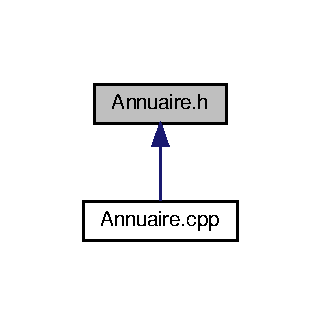
\includegraphics[width=154pt]{Annuaire_8h__dep__incl}
\end{center}
\end{figure}
\subsection*{Classes}
\begin{DoxyCompactItemize}
\item 
class \hyperlink{classhockey_1_1Annuaire}{hockey\+::\+Annuaire}
\begin{DoxyCompactList}\small\item\em Cette classe sert à la gestion des personnes membres d\textquotesingle{}une équipe de hockey. \end{DoxyCompactList}\end{DoxyCompactItemize}


\subsection{Detailed Description}
\+: Fichier qui contient l\textquotesingle{}interface de la classe annuaire qui permet de faire la gestion des personnes membres d\textquotesingle{}une équipe de hockey dans un annuaire. 

Attributs\+:
\begin{DoxyItemize}
\item string m\+\_\+nom\+Club\+: Le nom de l\textquotesingle{}équipe de hockey.
\item vector$<$$\ast$\+Personne$>$ m\+\_\+v\+Membres\+: un vecteur contenant des pointeurs vers les personnes membres de l\textquotesingle{}équipe \begin{DoxyAuthor}{Author}
\+: Jordan Longval 
\end{DoxyAuthor}
\begin{DoxyVersion}{Version}
\+: T\+P3 
\end{DoxyVersion}
\begin{DoxyDate}{Date}
\+: 2020-\/04-\/02 
\end{DoxyDate}

\end{DoxyItemize}
\hypertarget{ContratException_8cpp}{}\section{Contrat\+Exception.\+cpp File Reference}
\label{ContratException_8cpp}\index{Contrat\+Exception.\+cpp@{Contrat\+Exception.\+cpp}}


Implantation de la classe \hyperlink{classContratException}{Contrat\+Exception} et de ses héritiers.  


{\ttfamily \#include \char`\"{}Contrat\+Exception.\+h\char`\"{}}\newline
{\ttfamily \#include $<$sstream$>$}\newline
{\ttfamily \#include $<$iostream$>$}\newline
Include dependency graph for Contrat\+Exception.\+cpp\+:\nopagebreak
\begin{figure}[H]
\begin{center}
\leavevmode
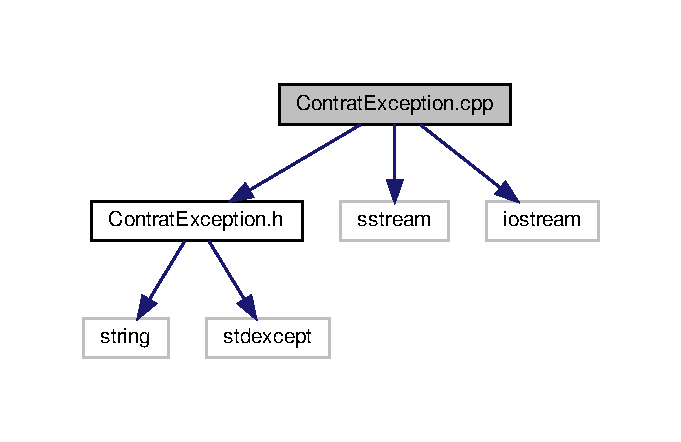
\includegraphics[width=327pt]{ContratException_8cpp__incl}
\end{center}
\end{figure}


\subsection{Detailed Description}
Implantation de la classe \hyperlink{classContratException}{Contrat\+Exception} et de ses héritiers. 

\begin{DoxyAuthor}{Author}
administrateur 
\end{DoxyAuthor}

\hypertarget{ContratException_8h}{}\section{Contrat\+Exception.\+h File Reference}
\label{ContratException_8h}\index{Contrat\+Exception.\+h@{Contrat\+Exception.\+h}}


Fichier contenant la déclaration de la classe \hyperlink{classContratException}{Contrat\+Exception} et de ses héritiers.  


{\ttfamily \#include $<$string$>$}\newline
{\ttfamily \#include $<$stdexcept$>$}\newline
Include dependency graph for Contrat\+Exception.\+h\+:\nopagebreak
\begin{figure}[H]
\begin{center}
\leavevmode
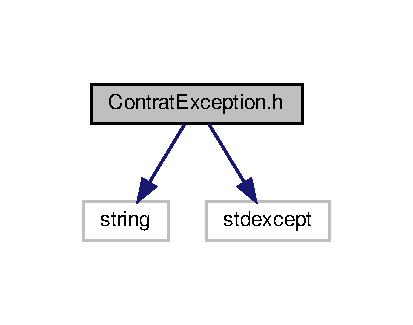
\includegraphics[width=198pt]{ContratException_8h__incl}
\end{center}
\end{figure}
This graph shows which files directly or indirectly include this file\+:\nopagebreak
\begin{figure}[H]
\begin{center}
\leavevmode
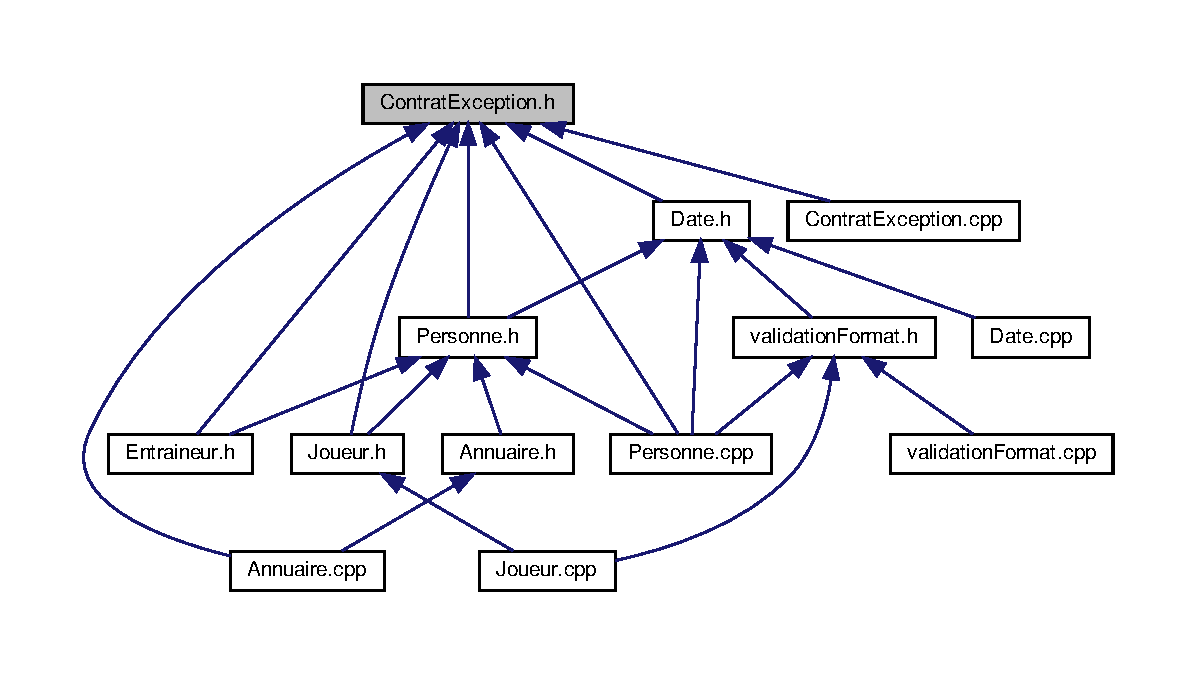
\includegraphics[width=350pt]{ContratException_8h__dep__incl}
\end{center}
\end{figure}
\subsection*{Classes}
\begin{DoxyCompactItemize}
\item 
class \hyperlink{classContratException}{Contrat\+Exception}
\begin{DoxyCompactList}\small\item\em Classe de base des exceptions de contrat. \end{DoxyCompactList}\item 
class \hyperlink{classAssertionException}{Assertion\+Exception}
\begin{DoxyCompactList}\small\item\em Classe pour la gestion des erreurs d\textquotesingle{}assertion. \end{DoxyCompactList}\item 
class \hyperlink{classPreconditionException}{Precondition\+Exception}
\begin{DoxyCompactList}\small\item\em Classe pour la gestion des erreurs de précondition. \end{DoxyCompactList}\item 
class \hyperlink{classPostconditionException}{Postcondition\+Exception}
\begin{DoxyCompactList}\small\item\em Classe pour la gestion des erreurs de postcondition. \end{DoxyCompactList}\item 
class \hyperlink{classInvariantException}{Invariant\+Exception}
\begin{DoxyCompactList}\small\item\em Classe pour la gestion des erreurs d\textquotesingle{}invariant. \end{DoxyCompactList}\end{DoxyCompactItemize}
\subsection*{Macros}
\begin{DoxyCompactItemize}
\item 
\mbox{\Hypertarget{ContratException_8h_a52dddc2c198c58b53b201c313934e40c}\label{ContratException_8h_a52dddc2c198c58b53b201c313934e40c}} 
\#define {\bfseries I\+N\+V\+A\+R\+I\+A\+N\+TS}()~verifie\+Invariant()
\item 
\mbox{\Hypertarget{ContratException_8h_abe6e3e0ff48f8595570e6485b506a8c4}\label{ContratException_8h_abe6e3e0ff48f8595570e6485b506a8c4}} 
\#define {\bfseries A\+S\+S\+E\+R\+T\+I\+ON}(f)~if (!(f)) throw \hyperlink{classAssertionException}{Assertion\+Exception}(\+\_\+\+\_\+\+F\+I\+L\+E\+\_\+\+\_\+,\+\_\+\+\_\+\+L\+I\+N\+E\+\_\+\+\_\+, \#f);
\item 
\mbox{\Hypertarget{ContratException_8h_acb3361bd87fc697a57b7286a9998c106}\label{ContratException_8h_acb3361bd87fc697a57b7286a9998c106}} 
\#define {\bfseries P\+R\+E\+C\+O\+N\+D\+I\+T\+I\+ON}(f)~if (!(f)) throw \hyperlink{classPreconditionException}{Precondition\+Exception}(\+\_\+\+\_\+\+F\+I\+L\+E\+\_\+\+\_\+, \+\_\+\+\_\+\+L\+I\+N\+E\+\_\+\+\_\+, \#f);
\item 
\mbox{\Hypertarget{ContratException_8h_a438b75c0c77a1ce8d1e914f9f04ea548}\label{ContratException_8h_a438b75c0c77a1ce8d1e914f9f04ea548}} 
\#define {\bfseries P\+O\+S\+T\+C\+O\+N\+D\+I\+T\+I\+ON}(f)~if (!(f)) throw \hyperlink{classPostconditionException}{Postcondition\+Exception}(\+\_\+\+\_\+\+F\+I\+L\+E\+\_\+\+\_\+, \+\_\+\+\_\+\+L\+I\+N\+E\+\_\+\+\_\+, \#f);
\item 
\mbox{\Hypertarget{ContratException_8h_a08f80155f47e05681c2b9bb9c5f6fffe}\label{ContratException_8h_a08f80155f47e05681c2b9bb9c5f6fffe}} 
\#define {\bfseries I\+N\+V\+A\+R\+I\+A\+NT}(f)~if (!(f)) throw \hyperlink{classInvariantException}{Invariant\+Exception}(\+\_\+\+\_\+\+F\+I\+L\+E\+\_\+\+\_\+,\+\_\+\+\_\+\+L\+I\+N\+E\+\_\+\+\_\+, \#f);
\end{DoxyCompactItemize}


\subsection{Detailed Description}
Fichier contenant la déclaration de la classe \hyperlink{classContratException}{Contrat\+Exception} et de ses héritiers. 

\begin{DoxyAuthor}{Author}
administrateur 
\end{DoxyAuthor}

\hypertarget{Date_8cpp}{}\section{Date.\+cpp File Reference}
\label{Date_8cpp}\index{Date.\+cpp@{Date.\+cpp}}


Implantation de la classe Date révision \+: normes 12-\/2013 balises Doxygen révision des commentaires de spécification d\textquotesingle{}en-\/tête des méthodes.  


{\ttfamily \#include \char`\"{}Date.\+h\char`\"{}}\newline
{\ttfamily \#include $<$sstream$>$}\newline
{\ttfamily \#include $<$ctime$>$}\newline
{\ttfamily \#include $<$iostream$>$}\newline
Include dependency graph for Date.\+cpp\+:\nopagebreak
\begin{figure}[H]
\begin{center}
\leavevmode
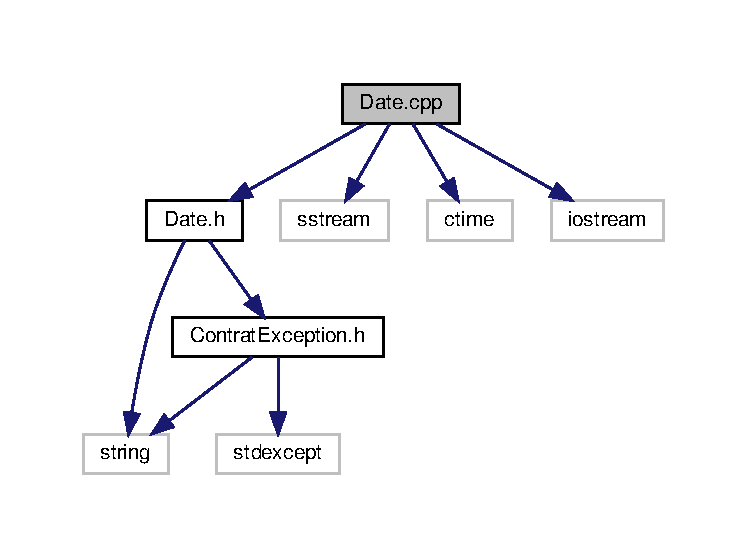
\includegraphics[width=350pt]{Date_8cpp__incl}
\end{center}
\end{figure}


\subsection{Detailed Description}
Implantation de la classe Date révision \+: normes 12-\/2013 balises Doxygen révision des commentaires de spécification d\textquotesingle{}en-\/tête des méthodes. 

\begin{DoxyAuthor}{Author}
Yves Roy Version initiale, T\+HE 
\end{DoxyAuthor}
\begin{DoxyDate}{Date}
28 octobre 2016 
\end{DoxyDate}
\begin{DoxyVersion}{Version}
2.\+4 
\end{DoxyVersion}

\hypertarget{Date_8h}{}\section{Date.\+h File Reference}
\label{Date_8h}\index{Date.\+h@{Date.\+h}}


Fichier qui contient l\textquotesingle{}interface de la classe Date qui sert au maintien et à la manipulation des dates.  


{\ttfamily \#include \char`\"{}Contrat\+Exception.\+h\char`\"{}}\newline
{\ttfamily \#include $<$string$>$}\newline
Include dependency graph for Date.\+h\+:\nopagebreak
\begin{figure}[H]
\begin{center}
\leavevmode
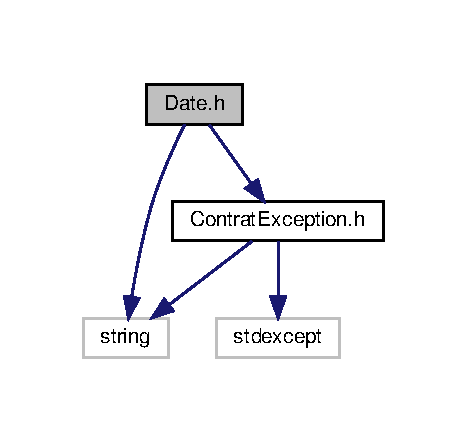
\includegraphics[width=224pt]{Date_8h__incl}
\end{center}
\end{figure}
This graph shows which files directly or indirectly include this file\+:\nopagebreak
\begin{figure}[H]
\begin{center}
\leavevmode
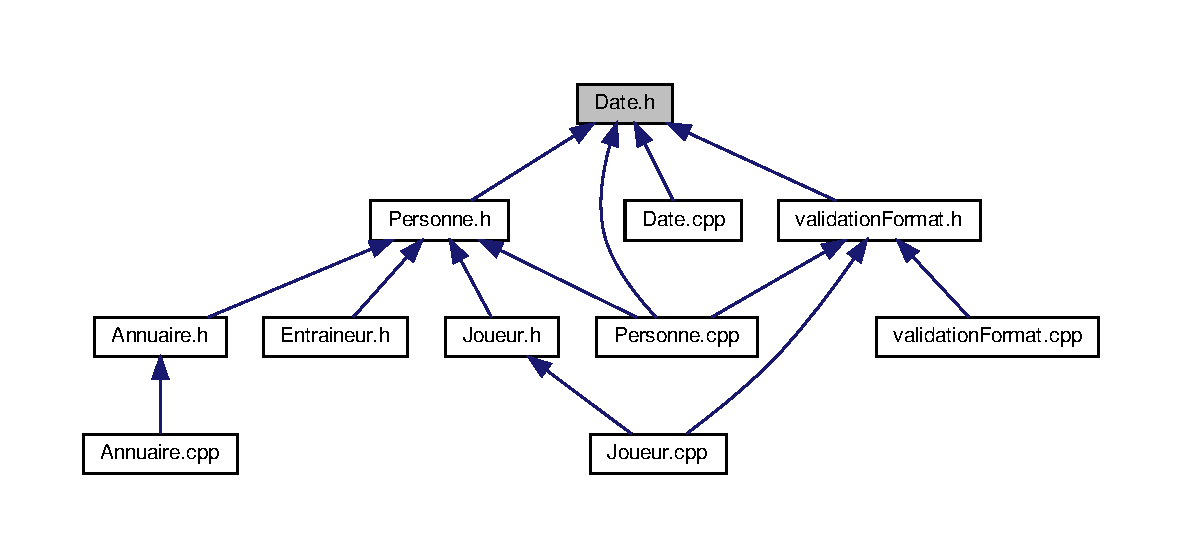
\includegraphics[width=350pt]{Date_8h__dep__incl}
\end{center}
\end{figure}
\subsection*{Classes}
\begin{DoxyCompactItemize}
\item 
class \hyperlink{classutil_1_1Date}{util\+::\+Date}
\begin{DoxyCompactList}\small\item\em Cette classe sert au maintien et à la manipulation des dates. \end{DoxyCompactList}\end{DoxyCompactItemize}


\subsection{Detailed Description}
Fichier qui contient l\textquotesingle{}interface de la classe Date qui sert au maintien et à la manipulation des dates. 

\begin{DoxyAuthor}{Author}
Yves Roy Version initiale, T\+HE 
\end{DoxyAuthor}
\begin{DoxyDate}{Date}
28 octobre 2016 
\end{DoxyDate}
\begin{DoxyVersion}{Version}
2.\+2 
\end{DoxyVersion}

\hypertarget{Entraineur_8h}{}\section{Entraineur.\+h File Reference}
\label{Entraineur_8h}\index{Entraineur.\+h@{Entraineur.\+h}}


Fichier contenant l\textquotesingle{}implémentation de la classe Entraineur. Cette classe est dérivée de la classe Personne. Attributs\+: -\/string m\+\_\+num\+R\+A\+MQ\+: le numéro de R\+A\+MQ de la personne dans le format standard suivant N\+N\+NP A\+A\+MM J\+J\+XX où NN sont les trois premières lettres du nom de famille de la personne en Maj, P est la première lettre du prénom de la personne en Maj, AA sont les deux derniers chiffres de l\textquotesingle{}année de naissance de la personne MM sont les chiffres du mois de naissance de la personne JJ sont les chiffres du jour de naissance de la personne XX est un code administratif dont on ne connait pas la valeur. -\/char m\+\_\+sexe\+: le sexe de l\textquotesingle{}entraîneur (\textquotesingle{}M\textquotesingle{} ou \textquotesingle{}F\textquotesingle{})  


{\ttfamily \#include \char`\"{}Personne.\+h\char`\"{}}\newline
{\ttfamily \#include \char`\"{}Contrat\+Exception.\+h\char`\"{}}\newline
Include dependency graph for Entraineur.\+h\+:\nopagebreak
\begin{figure}[H]
\begin{center}
\leavevmode
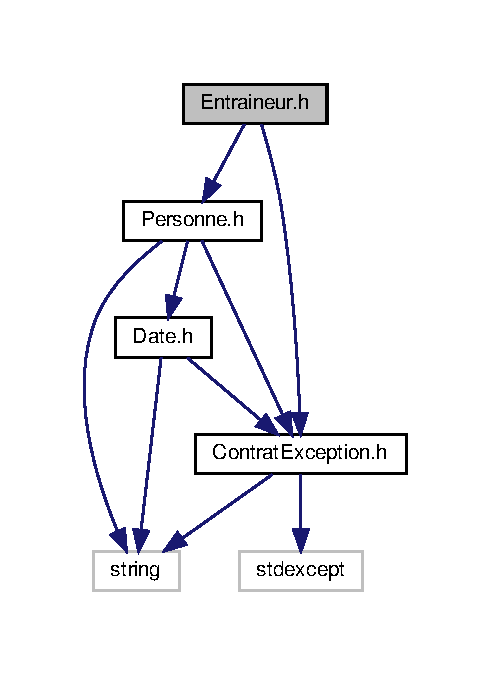
\includegraphics[width=235pt]{Entraineur_8h__incl}
\end{center}
\end{figure}
\subsection*{Classes}
\begin{DoxyCompactItemize}
\item 
class \hyperlink{classhockey_1_1Entraineur}{hockey\+::\+Entraineur}
\begin{DoxyCompactList}\small\item\em Cette classe sert au maintien et à la manipulation des entraineurs. Elle hérite de la classe \hyperlink{classhockey_1_1Personne}{Personne}. \end{DoxyCompactList}\end{DoxyCompactItemize}


\subsection{Detailed Description}
Fichier contenant l\textquotesingle{}implémentation de la classe Entraineur. Cette classe est dérivée de la classe Personne. Attributs\+: -\/string m\+\_\+num\+R\+A\+MQ\+: le numéro de R\+A\+MQ de la personne dans le format standard suivant N\+N\+NP A\+A\+MM J\+J\+XX où NN sont les trois premières lettres du nom de famille de la personne en Maj, P est la première lettre du prénom de la personne en Maj, AA sont les deux derniers chiffres de l\textquotesingle{}année de naissance de la personne MM sont les chiffres du mois de naissance de la personne JJ sont les chiffres du jour de naissance de la personne XX est un code administratif dont on ne connait pas la valeur. -\/char m\+\_\+sexe\+: le sexe de l\textquotesingle{}entraîneur (\textquotesingle{}M\textquotesingle{} ou \textquotesingle{}F\textquotesingle{}) 

Fichier contenant l\textquotesingle{}interface de la classe Entraineur. Cette classe est dérivée de la classe Personne. Attributs\+: -\/string m\+\_\+num\+R\+A\+MQ\+: le numéro de R\+A\+MQ de la personne dans le format standard suivant N\+N\+NP A\+A\+MM J\+J\+XX où NN sont les trois premières lettres du nom de famille de la personne en Maj, P est la première lettre du prénom de la personne en Maj, AA sont les deux derniers chiffres de l\textquotesingle{}année de naissance de la personne MM sont les chiffres du mois de naissance de la personne JJ sont les chiffres du jour de naissance de la personne XX est un code administratif dont on ne connait pas la valeur. -\/char m\+\_\+sexe\+: le sexe de l\textquotesingle{}entraîneur (\textquotesingle{}M\textquotesingle{} ou \textquotesingle{}F\textquotesingle{})

Note\+: L\textquotesingle{}entraîneur doit être majeur pour être valide.

\begin{DoxyAuthor}{Author}
\+: Jordan Longval 
\end{DoxyAuthor}
\begin{DoxyDate}{Date}
\+: 2020-\/04-\/02 
\end{DoxyDate}

\hypertarget{Joueur_8cpp}{}\section{Joueur.\+cpp File Reference}
\label{Joueur_8cpp}\index{Joueur.\+cpp@{Joueur.\+cpp}}
{\ttfamily \#include \char`\"{}Joueur.\+h\char`\"{}}\newline
{\ttfamily \#include \char`\"{}validation\+Format.\+h\char`\"{}}\newline
{\ttfamily \#include $<$string$>$}\newline
{\ttfamily \#include $<$sstream$>$}\newline
{\ttfamily \#include $<$iomanip$>$}\newline
Include dependency graph for Joueur.\+cpp\+:\nopagebreak
\begin{figure}[H]
\begin{center}
\leavevmode
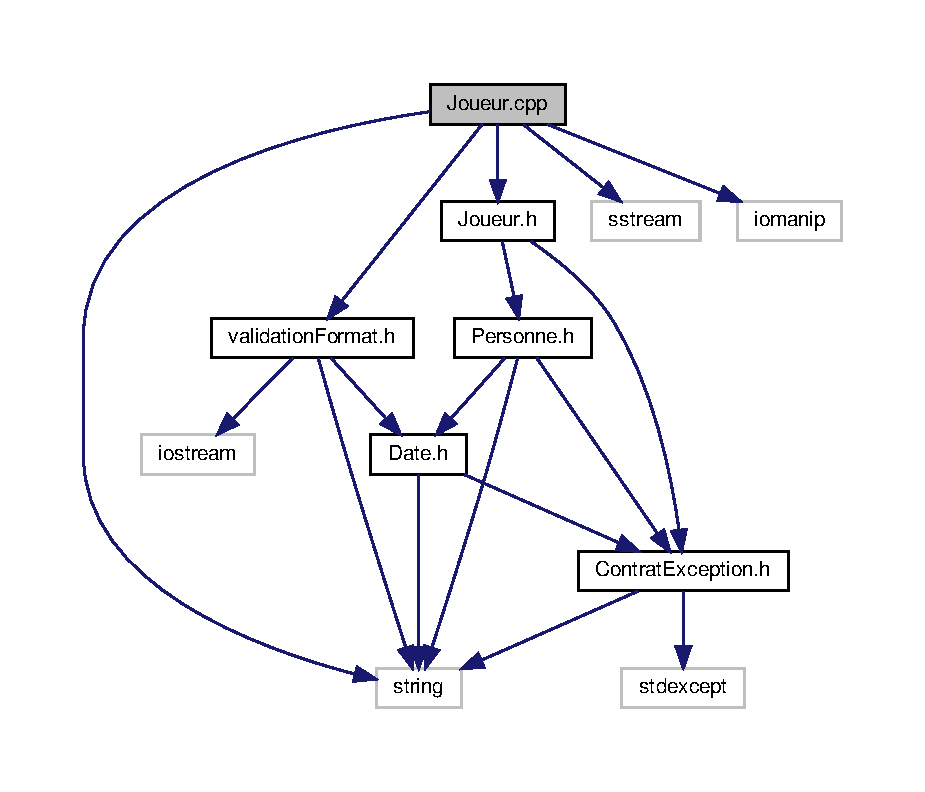
\includegraphics[width=350pt]{Joueur_8cpp__incl}
\end{center}
\end{figure}


\subsection{Detailed Description}
\begin{DoxyDate}{Date}
\+: 2020-\/04-\/02 
\end{DoxyDate}
\begin{DoxyAuthor}{Author}
\+: etudiant 
\end{DoxyAuthor}

\hypertarget{Joueur_8h}{}\section{Joueur.\+h File Reference}
\label{Joueur_8h}\index{Joueur.\+h@{Joueur.\+h}}
{\ttfamily \#include \char`\"{}Personne.\+h\char`\"{}}\newline
{\ttfamily \#include \char`\"{}Contrat\+Exception.\+h\char`\"{}}\newline
Include dependency graph for Joueur.\+h\+:\nopagebreak
\begin{figure}[H]
\begin{center}
\leavevmode
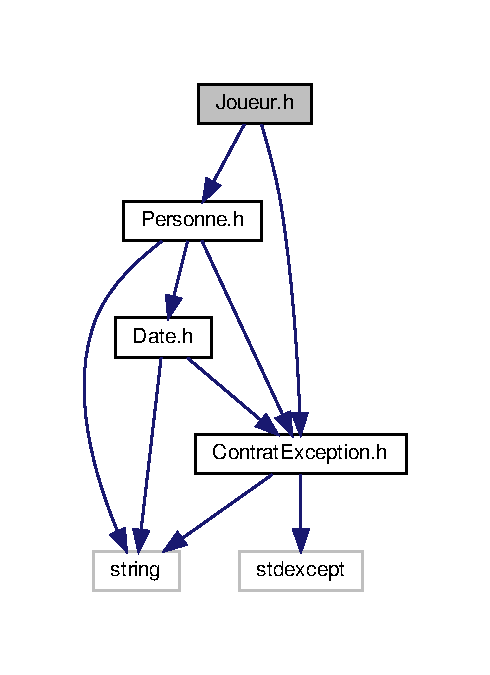
\includegraphics[width=235pt]{Joueur_8h__incl}
\end{center}
\end{figure}
This graph shows which files directly or indirectly include this file\+:\nopagebreak
\begin{figure}[H]
\begin{center}
\leavevmode
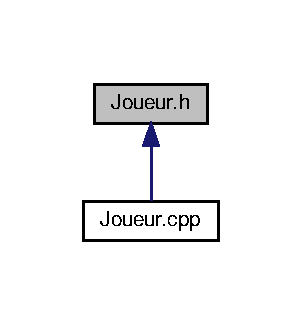
\includegraphics[width=145pt]{Joueur_8h__dep__incl}
\end{center}
\end{figure}
\subsection*{Classes}
\begin{DoxyCompactItemize}
\item 
class \hyperlink{classhockey_1_1Joueur}{hockey\+::\+Joueur}
\begin{DoxyCompactList}\small\item\em Cette classe sert au maintien et à la manipulation des joueurs. Elle hérite de la classe \hyperlink{classhockey_1_1Personne}{Personne}. \end{DoxyCompactList}\end{DoxyCompactItemize}


\subsection{Detailed Description}
\begin{DoxyDate}{Date}
\+: 2020-\/04-\/02 
\end{DoxyDate}
\begin{DoxyAuthor}{Author}
\+: etudiant 
\end{DoxyAuthor}

\hypertarget{Personne_8cpp}{}\section{Personne.\+cpp File Reference}
\label{Personne_8cpp}\index{Personne.\+cpp@{Personne.\+cpp}}


Cette classe sert au maintien et à la manipulation des personnes. Cette classe est abstraite.  


{\ttfamily \#include \char`\"{}Date.\+h\char`\"{}}\newline
{\ttfamily \#include \char`\"{}Personne.\+h\char`\"{}}\newline
{\ttfamily \#include \char`\"{}validation\+Format.\+h\char`\"{}}\newline
{\ttfamily \#include \char`\"{}Contrat\+Exception.\+h\char`\"{}}\newline
{\ttfamily \#include $<$sstream$>$}\newline
{\ttfamily \#include $<$iomanip$>$}\newline
Include dependency graph for Personne.\+cpp\+:\nopagebreak
\begin{figure}[H]
\begin{center}
\leavevmode
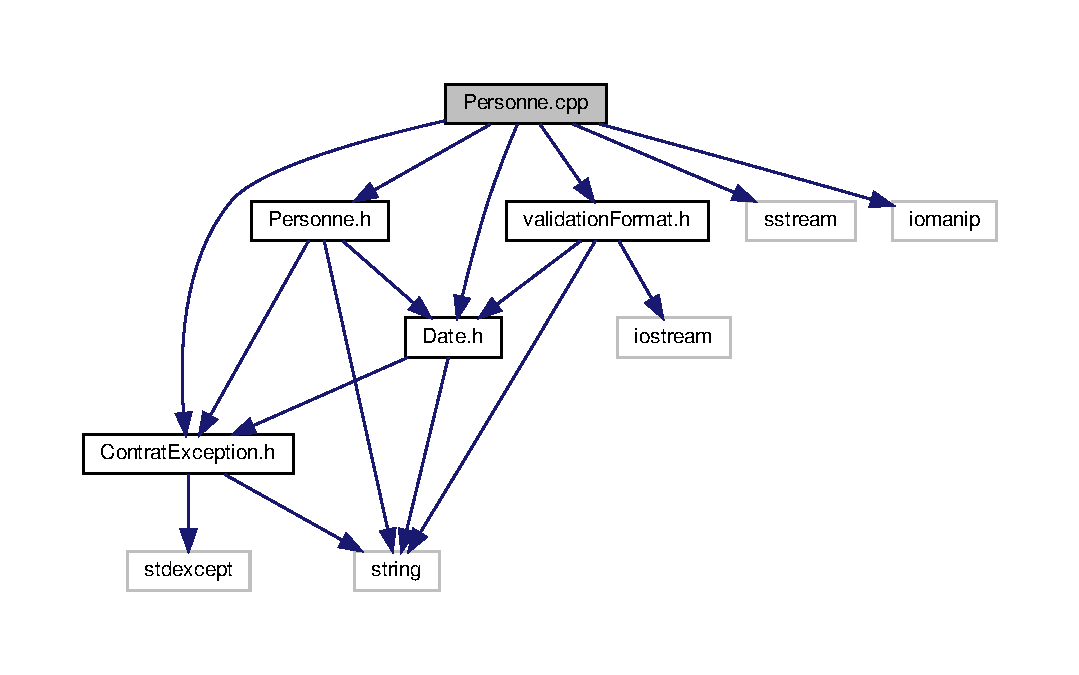
\includegraphics[width=350pt]{Personne_8cpp__incl}
\end{center}
\end{figure}


\subsection{Detailed Description}
Cette classe sert au maintien et à la manipulation des personnes. Cette classe est abstraite. 

Les valeurs qui entrent dans la classe doivent être validée à priori. 

Attributs\+: string p\+\_\+nom, string p\+\_\+prenom, Date p\+\_\+date\+Naissance, string p\+\_\+telephone \begin{DoxyAuthor}{Author}
Jordan Longval 
\end{DoxyAuthor}

\hypertarget{Personne_8h}{}\section{Personne.\+h File Reference}
\label{Personne_8h}\index{Personne.\+h@{Personne.\+h}}


Fichier qui contient l\textquotesingle{}interface de la classe abstraite Personne qui permet de récolter les informations d\textquotesingle{}une personne.  


{\ttfamily \#include \char`\"{}Date.\+h\char`\"{}}\newline
{\ttfamily \#include \char`\"{}string\char`\"{}}\newline
{\ttfamily \#include \char`\"{}Contrat\+Exception.\+h\char`\"{}}\newline
Include dependency graph for Personne.\+h\+:\nopagebreak
\begin{figure}[H]
\begin{center}
\leavevmode
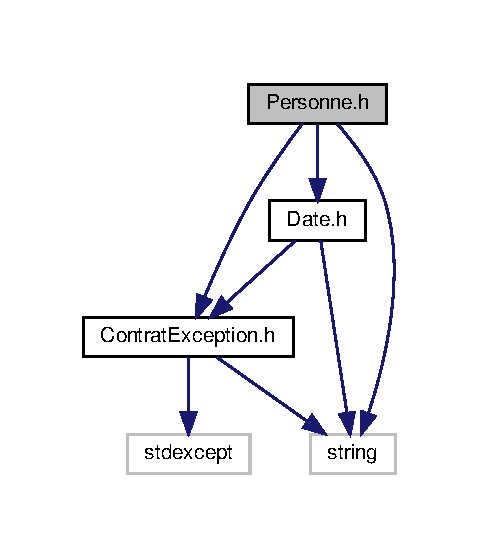
\includegraphics[width=230pt]{Personne_8h__incl}
\end{center}
\end{figure}
This graph shows which files directly or indirectly include this file\+:\nopagebreak
\begin{figure}[H]
\begin{center}
\leavevmode
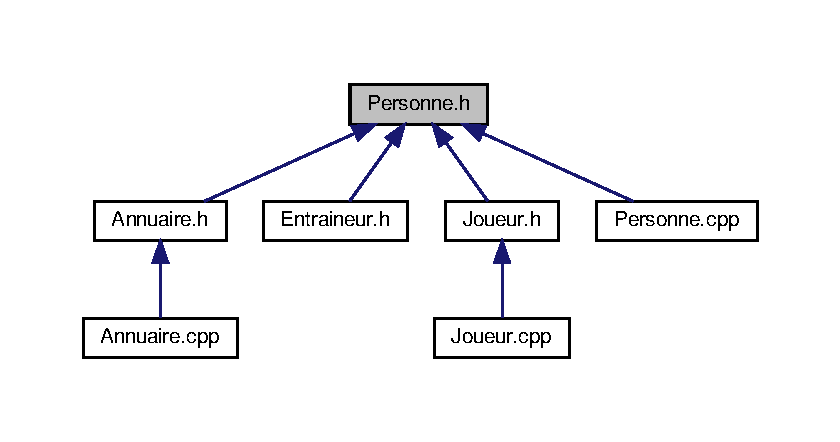
\includegraphics[width=350pt]{Personne_8h__dep__incl}
\end{center}
\end{figure}
\subsection*{Classes}
\begin{DoxyCompactItemize}
\item 
class \hyperlink{classhockey_1_1Personne}{hockey\+::\+Personne}
\begin{DoxyCompactList}\small\item\em Cette classe sert au maintien et à la manipulation des personnes. \end{DoxyCompactList}\end{DoxyCompactItemize}


\subsection{Detailed Description}
Fichier qui contient l\textquotesingle{}interface de la classe abstraite Personne qui permet de récolter les informations d\textquotesingle{}une personne. 

\begin{DoxyAuthor}{Author}
Jordan Longval 
\end{DoxyAuthor}
\begin{DoxyVersion}{Version}
T\+P3 
\end{DoxyVersion}
\begin{DoxyDate}{Date}

\end{DoxyDate}

\hypertarget{validationFormat_8cpp}{}\section{validation\+Format.\+cpp File Reference}
\label{validationFormat_8cpp}\index{validation\+Format.\+cpp@{validation\+Format.\+cpp}}


Ce fichier comporte les fonctions permettant de valider le numéro de téléphone standard canadien au niveau national ainsi que le numéro de la R\+A\+MQ.  


{\ttfamily \#include \char`\"{}validation\+Format.\+h\char`\"{}}\newline
{\ttfamily \#include $<$iostream$>$}\newline
Include dependency graph for validation\+Format.\+cpp\+:\nopagebreak
\begin{figure}[H]
\begin{center}
\leavevmode
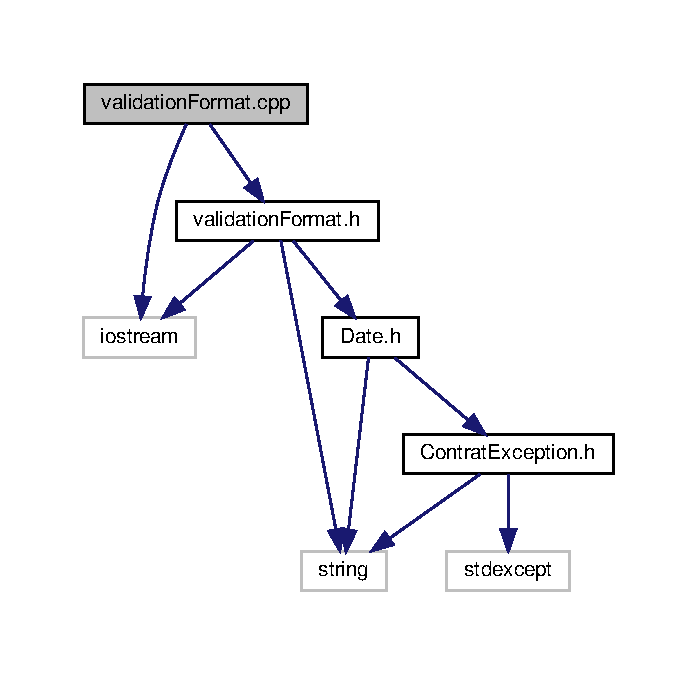
\includegraphics[width=334pt]{validationFormat_8cpp__incl}
\end{center}
\end{figure}
\subsection*{Functions}
\begin{DoxyCompactItemize}
\item 
bool \hyperlink{validationFormat_8cpp_ad19b58e0318b66129069390b2da7496e}{util\+::valider\+Telephone} (const std\+::string \&p\+\_\+telephone)
\begin{DoxyCompactList}\small\item\em Valide le format d\textquotesingle{}un numéro de téléphone pour qu\textquotesingle{}il respecte le format national canadien standard. \end{DoxyCompactList}\item 
bool \hyperlink{validationFormat_8cpp_a5743386c1cc811ee37f66a9c58162ff5}{util\+::verification\+Longueur\+Tel} (const std\+::string \&p\+\_\+telephone)
\begin{DoxyCompactList}\small\item\em Vérifie que le string du numéro de téléphone est de la bonne longueur. \end{DoxyCompactList}\item 
bool \hyperlink{validationFormat_8cpp_a91d98db549a5328db80783a9cb5a3811}{util\+::verification\+Espace\+Trait} (const std\+::string \&p\+\_\+telephone)
\begin{DoxyCompactList}\small\item\em Vérifie que le numéro contient un espace et un trait et qu\textquotesingle{}ils sont aux bons endroits. \end{DoxyCompactList}\item 
bool \hyperlink{validationFormat_8cpp_a00b57c98b926a63daa8215e1436b63dc}{util\+::verification\+Chiffres} (const std\+::string \&p\+\_\+telephone)
\begin{DoxyCompactList}\small\item\em Vérifie que le numéro ne contient que des chiffres (à l\textquotesingle{}exception de l\textquotesingle{}espace et du trait) \end{DoxyCompactList}\item 
bool \hyperlink{validationFormat_8cpp_a06d6b26422f8b93767e39482e237c75c}{util\+::verification\+Indicatif} (const std\+::string \&p\+\_\+telephone)
\begin{DoxyCompactList}\small\item\em Vérifie que l\textquotesingle{}indicatif du numéro est un indicatif valide. Pour ce faire le programme vérifie dans un tableau d\textquotesingle{}indicatifs acceptés I\+N\+D\+I\+C\+A\+T\+I\+F\+S\+\_\+\+A\+C\+C\+E\+P\+T\+ES\mbox{[}\mbox{]} ou encore accepte l\textquotesingle{}indicatif s\textquotesingle{}il commence par un 9. \end{DoxyCompactList}\item 
bool \hyperlink{validationFormat_8cpp_a25f8d52b23785c48a5256d8b66ab466d}{util\+::valider\+Num\+R\+A\+MQ} (const std\+::string \&p\+\_\+numero, const std\+::string \&p\+\_\+nom, const std\+::string \&p\+\_\+prenom, int p\+\_\+jour\+Naissance, int p\+\_\+mois\+Naissance, int p\+\_\+annee\+Naissance, char p\+\_\+sexe)
\begin{DoxyCompactList}\small\item\em Vérifie qu\textquotesingle{}un numéro de R\+A\+MQ fourni sous forme de string respecte le format standard et qu\textquotesingle{}il concorde avec les autres informations fournies. Le format standard est les suivant N\+N\+NP A\+A\+MM J\+J\+XX où NN sont les trois premières lettres du nom de famille de la personne en Maj, P est la première lettre du prénom de la personne en Maj, AA sont les deux derniers chiffres de l\textquotesingle{}année de naissance de la personne MM sont les chiffres du mois de naissance de la personne JJ sont les chiffres du jour de naissance de la personne XX est un code administratif dont on ne connait pas la valeur. \end{DoxyCompactList}\item 
bool \hyperlink{validationFormat_8cpp_a79c9909ab5b1e969dc6b2f77d966eb6c}{util\+::verification\+Longueur\+R\+A\+MQ} (const std\+::string \&p\+\_\+numero)
\begin{DoxyCompactList}\small\item\em Vérifie que le numéro de la R\+A\+MQ fournie est de la bonne longueur. \end{DoxyCompactList}\item 
bool \hyperlink{validationFormat_8cpp_a6046ececaf0ad6874e7a9b76a797ff44}{util\+::verification\+Position\+Espaces\+R\+A\+MQ} (const std\+::string \&p\+\_\+numero)
\begin{DoxyCompactList}\small\item\em Vérifie que le numéro de la R\+A\+MQ fournie possède deux espaces qui sont aux bons endroits. \end{DoxyCompactList}\item 
bool \hyperlink{validationFormat_8cpp_a8515bea07b4b8021d249d03d6626b7ee}{util\+::verification\+Nom\+R\+A\+MQ} (const std\+::string \&p\+\_\+numero, const std\+::string \&p\+\_\+nom)
\begin{DoxyCompactList}\small\item\em Vérifie que le numéro de la R\+A\+MQ fournie concorde avec le nom de la personne. \end{DoxyCompactList}\item 
bool \hyperlink{validationFormat_8cpp_af22d126590f7a04264c228a2dc1f1dca}{util\+::verification\+Prenom\+R\+A\+MQ} (const std\+::string \&p\+\_\+numero, const std\+::string \&p\+\_\+prenom)
\begin{DoxyCompactList}\small\item\em Vérifie que le numéro de la R\+A\+MQ fournie concorde avec le prénom de la personne. \end{DoxyCompactList}\item 
bool \hyperlink{validationFormat_8cpp_ac1410e9900e443039e04492a9dcb51ae}{util\+::verification\+Annee\+R\+A\+MQ} (const std\+::string \&p\+\_\+numero, const int p\+\_\+annee\+Naissance)
\begin{DoxyCompactList}\small\item\em Vérifie que le numéro de la R\+A\+MQ fournie concorde avec l\textquotesingle{}année de naissance de la personne. \end{DoxyCompactList}\item 
bool \hyperlink{validationFormat_8cpp_a6b46e2eb29fab39a4b3df7c6c703b3b3}{util\+::verification\+Mois\+R\+A\+MQ} (const std\+::string \&p\+\_\+numero, const int p\+\_\+mois\+Naissance, char \&p\+\_\+sexe)
\begin{DoxyCompactList}\small\item\em Vérifie que le numéro de la R\+A\+MQ fournie concorde avec le mois de naissance de la personne. \end{DoxyCompactList}\item 
bool \hyperlink{validationFormat_8cpp_a9188427a80c9811cb9cac0432584a097}{util\+::verification\+Jour\+R\+A\+MQ} (const std\+::string \&p\+\_\+numero, int p\+\_\+jour\+Naissance)
\begin{DoxyCompactList}\small\item\em Vérifie que le numéro de la R\+A\+MQ fournie concorde avec le jour de naissance de la personne. \end{DoxyCompactList}\item 
std\+::string \hyperlink{validationFormat_8cpp_a9725447dd2572abb047af57c0101793f}{util\+::transfo\+Majuscule} (const std\+::string \&p\+\_\+chaine\+A\+Changer)
\begin{DoxyCompactList}\small\item\em Fonction qui prend un string en entrée et donne en sortie un string majuscule du string d\textquotesingle{}entrée. \end{DoxyCompactList}\item 
bool \hyperlink{validationFormat_8cpp_ab3d93e73408df98688844f00a8cdce58}{util\+::valider\+Format\+Nom} (const std\+::string \&p\+\_\+nom)
\begin{DoxyCompactList}\small\item\em Vérifie que le nom donné ne contient que des lettres (maj ou min) et n\textquotesingle{}est pas vide. \end{DoxyCompactList}\item 
bool \hyperlink{validationFormat_8cpp_a0f4b6c8097b37ec3712dc34d2363a083}{util\+::valider\+Sexe} (const char \&p\+\_\+sexe)
\begin{DoxyCompactList}\small\item\em Vérifie que le sexe donné en entrée est soit \textquotesingle{}M\textquotesingle{},\textquotesingle{}m\textquotesingle{},\textquotesingle{}F\textquotesingle{} ou \textquotesingle{}f\textquotesingle{}. \end{DoxyCompactList}\item 
bool \hyperlink{validationFormat_8cpp_afc8b13ca75c2d31a81d2cff1e9ae7d7c}{util\+::valider\+Position} (const std\+::string \&p\+\_\+position)
\begin{DoxyCompactList}\small\item\em Vérifie que la position en entrée est soit \char`\"{}centre\char`\"{},\char`\"{}ailier\char`\"{},\char`\"{}défenseur\char`\"{} ou \char`\"{}gardien\char`\"{}. \end{DoxyCompactList}\item 
bool \hyperlink{validationFormat_8cpp_abed031230a6601feb893f74fe783c5ff}{util\+::valider\+Age\+Entraineur} (const Date \&p\+\_\+date\+Naissance\+Entraineur)
\begin{DoxyCompactList}\small\item\em Vérifie que l\textquotesingle{}âge en entrée est supérieur à 18 ans. \end{DoxyCompactList}\item 
bool \hyperlink{validationFormat_8cpp_afef869875a75ed592e94ef4f02d08419}{util\+::valider\+Age\+Joueur} (const Date \&p\+\_\+date\+Naissance\+Joueur)
\begin{DoxyCompactList}\small\item\em Vérifie que l\textquotesingle{}âge en entrée est entre 15 et 17 ans. \end{DoxyCompactList}\end{DoxyCompactItemize}


\subsection{Detailed Description}
Ce fichier comporte les fonctions permettant de valider le numéro de téléphone standard canadien au niveau national ainsi que le numéro de la R\+A\+MQ. 

\begin{DoxyAuthor}{Author}
Jordan Longval 
\end{DoxyAuthor}
\begin{DoxyVersion}{Version}
1.\+0 
\end{DoxyVersion}
\begin{DoxyDate}{Date}
10/02/20 
\end{DoxyDate}


\subsection{Function Documentation}
\mbox{\Hypertarget{validationFormat_8cpp_file_a9725447dd2572abb047af57c0101793f}\label{validationFormat_8cpp_file_a9725447dd2572abb047af57c0101793f}} 
\index{validation\+Format.\+cpp@{validation\+Format.\+cpp}!transfo\+Majuscule@{transfo\+Majuscule}}
\index{transfo\+Majuscule@{transfo\+Majuscule}!validation\+Format.\+cpp@{validation\+Format.\+cpp}}
\subsubsection{\texorpdfstring{transfo\+Majuscule()}{transfoMajuscule()}}
{\footnotesize\ttfamily std\+::string util\+::transfo\+Majuscule (\begin{DoxyParamCaption}\item[{const std\+::string \&}]{p\+\_\+chaine\+A\+Changer }\end{DoxyParamCaption})}



Fonction qui prend un string en entrée et donne en sortie un string majuscule du string d\textquotesingle{}entrée. 


\begin{DoxyParams}[1]{Parameters}
\mbox{\tt in}  & {\em p\+\_\+chaine\+A\+Changer} & un string que l\textquotesingle{}on veut mettre complètement en majuscule \\
\hline
\end{DoxyParams}
\begin{DoxyPrecond}{Precondition}
p\+\_\+chaine\+A\+Changer ne doit contenir que des lettres de a à z ou A à Z. 
\end{DoxyPrecond}
\begin{DoxyReturn}{Returns}
un string contenant la version majuscule de la chaine à changer. 
\end{DoxyReturn}
\mbox{\Hypertarget{validationFormat_8cpp_file_abed031230a6601feb893f74fe783c5ff}\label{validationFormat_8cpp_file_abed031230a6601feb893f74fe783c5ff}} 
\index{validation\+Format.\+cpp@{validation\+Format.\+cpp}!valider\+Age\+Entraineur@{valider\+Age\+Entraineur}}
\index{valider\+Age\+Entraineur@{valider\+Age\+Entraineur}!validation\+Format.\+cpp@{validation\+Format.\+cpp}}
\subsubsection{\texorpdfstring{valider\+Age\+Entraineur()}{validerAgeEntraineur()}}
{\footnotesize\ttfamily bool util\+::valider\+Age\+Entraineur (\begin{DoxyParamCaption}\item[{const \hyperlink{classutil_1_1Date}{Date} \&}]{p\+\_\+date\+Naissance\+Entraineur }\end{DoxyParamCaption})}



Vérifie que l\textquotesingle{}âge en entrée est supérieur à 18 ans. 


\begin{DoxyParams}[1]{Parameters}
\mbox{\tt in}  & {\em p\+\_\+date\+Naissance\+Entraineur} & la date de naissance à valider \\
\hline
\end{DoxyParams}
\begin{DoxyReturn}{Returns}
un bool qui est vrai lorsque les conditions sont satisfaites. 
\end{DoxyReturn}
\mbox{\Hypertarget{validationFormat_8cpp_file_afef869875a75ed592e94ef4f02d08419}\label{validationFormat_8cpp_file_afef869875a75ed592e94ef4f02d08419}} 
\index{validation\+Format.\+cpp@{validation\+Format.\+cpp}!valider\+Age\+Joueur@{valider\+Age\+Joueur}}
\index{valider\+Age\+Joueur@{valider\+Age\+Joueur}!validation\+Format.\+cpp@{validation\+Format.\+cpp}}
\subsubsection{\texorpdfstring{valider\+Age\+Joueur()}{validerAgeJoueur()}}
{\footnotesize\ttfamily bool util\+::valider\+Age\+Joueur (\begin{DoxyParamCaption}\item[{const \hyperlink{classutil_1_1Date}{Date} \&}]{p\+\_\+date\+Naissance\+Joueur }\end{DoxyParamCaption})}



Vérifie que l\textquotesingle{}âge en entrée est entre 15 et 17 ans. 


\begin{DoxyParams}[1]{Parameters}
\mbox{\tt in}  & {\em p\+\_\+date\+Naissance\+Joueur} & la date de naissance à valider \\
\hline
\end{DoxyParams}
\begin{DoxyReturn}{Returns}
un bool qui est vrai lorsque les conditions sont satisfaites. 
\end{DoxyReturn}
\mbox{\Hypertarget{validationFormat_8cpp_file_ab3d93e73408df98688844f00a8cdce58}\label{validationFormat_8cpp_file_ab3d93e73408df98688844f00a8cdce58}} 
\index{validation\+Format.\+cpp@{validation\+Format.\+cpp}!valider\+Format\+Nom@{valider\+Format\+Nom}}
\index{valider\+Format\+Nom@{valider\+Format\+Nom}!validation\+Format.\+cpp@{validation\+Format.\+cpp}}
\subsubsection{\texorpdfstring{valider\+Format\+Nom()}{validerFormatNom()}}
{\footnotesize\ttfamily bool util\+::valider\+Format\+Nom (\begin{DoxyParamCaption}\item[{const std\+::string \&}]{p\+\_\+nom }\end{DoxyParamCaption})}



Vérifie que le nom donné ne contient que des lettres (maj ou min) et n\textquotesingle{}est pas vide. 


\begin{DoxyParams}[1]{Parameters}
\mbox{\tt in}  & {\em p\+\_\+nom} & le nom à valider \\
\hline
\end{DoxyParams}
\begin{DoxyReturn}{Returns}
un bool qui est vrai lorsque le nom de contient que des lettres (Maj ou min) et n\textquotesingle{}est pas vide et faux si ce n\textquotesingle{}est pas le cas. 
\end{DoxyReturn}
\mbox{\Hypertarget{validationFormat_8cpp_file_a25f8d52b23785c48a5256d8b66ab466d}\label{validationFormat_8cpp_file_a25f8d52b23785c48a5256d8b66ab466d}} 
\index{validation\+Format.\+cpp@{validation\+Format.\+cpp}!valider\+Num\+R\+A\+MQ@{valider\+Num\+R\+A\+MQ}}
\index{valider\+Num\+R\+A\+MQ@{valider\+Num\+R\+A\+MQ}!validation\+Format.\+cpp@{validation\+Format.\+cpp}}
\subsubsection{\texorpdfstring{valider\+Num\+R\+A\+M\+Q()}{validerNumRAMQ()}}
{\footnotesize\ttfamily bool util\+::valider\+Num\+R\+A\+MQ (\begin{DoxyParamCaption}\item[{const std\+::string \&}]{p\+\_\+numero,  }\item[{const std\+::string \&}]{p\+\_\+nom,  }\item[{const std\+::string \&}]{p\+\_\+prenom,  }\item[{int}]{p\+\_\+jour\+Naissance,  }\item[{int}]{p\+\_\+mois\+Naissance,  }\item[{int}]{p\+\_\+annee\+Naissance,  }\item[{char}]{p\+\_\+sexe }\end{DoxyParamCaption})}



Vérifie qu\textquotesingle{}un numéro de R\+A\+MQ fourni sous forme de string respecte le format standard et qu\textquotesingle{}il concorde avec les autres informations fournies. Le format standard est les suivant N\+N\+NP A\+A\+MM J\+J\+XX où NN sont les trois premières lettres du nom de famille de la personne en Maj, P est la première lettre du prénom de la personne en Maj, AA sont les deux derniers chiffres de l\textquotesingle{}année de naissance de la personne MM sont les chiffres du mois de naissance de la personne JJ sont les chiffres du jour de naissance de la personne XX est un code administratif dont on ne connait pas la valeur. 


\begin{DoxyParams}[1]{Parameters}
\mbox{\tt in}  & {\em p\+\_\+numero} & Un string contenant le numéro de R\+A\+MQ à valider \\
\hline
\mbox{\tt in}  & {\em p\+\_\+nom} & Un string contenant le nom de la personne \\
\hline
\mbox{\tt in}  & {\em p\+\_\+prenom} & Un string contenant le prenom de la personne \\
\hline
\mbox{\tt in}  & {\em p\+\_\+jour\+Naissance} & un entier représentant le jour de naissance de la personne \\
\hline
\mbox{\tt in}  & {\em p\+\_\+mois\+Naissance} & un entier représentant le mois de naissance de la personne \\
\hline
\mbox{\tt in}  & {\em p\+\_\+annee\+Naissance} & un entier représentant les deux derniers chiffres de l\textquotesingle{}année de naissance de la personne \\
\hline
\mbox{\tt in}  & {\em p\+\_\+sexe} & un charactère représentant le sexe de la personne \\
\hline
\end{DoxyParams}
\begin{DoxyPrecond}{Precondition}
les valeurs p\+\_\+nom à p\+\_\+sex doivent être valides. les valeurs valides de p\+\_\+sex sont \textquotesingle{}m\textquotesingle{},\textquotesingle{}M\textquotesingle{},pour homme et \textquotesingle{}f\textquotesingle{},\textquotesingle{}F\textquotesingle{}, pour femme. 
\end{DoxyPrecond}
\begin{DoxyReturn}{Returns}
un bool qui est vrai lorsque le numéro de R\+A\+MQ est valide. et faux si ce n\textquotesingle{}est pas le cas. 
\end{DoxyReturn}
\mbox{\Hypertarget{validationFormat_8cpp_file_afc8b13ca75c2d31a81d2cff1e9ae7d7c}\label{validationFormat_8cpp_file_afc8b13ca75c2d31a81d2cff1e9ae7d7c}} 
\index{validation\+Format.\+cpp@{validation\+Format.\+cpp}!valider\+Position@{valider\+Position}}
\index{valider\+Position@{valider\+Position}!validation\+Format.\+cpp@{validation\+Format.\+cpp}}
\subsubsection{\texorpdfstring{valider\+Position()}{validerPosition()}}
{\footnotesize\ttfamily bool util\+::valider\+Position (\begin{DoxyParamCaption}\item[{const std\+::string \&}]{p\+\_\+position }\end{DoxyParamCaption})}



Vérifie que la position en entrée est soit \char`\"{}centre\char`\"{},\char`\"{}ailier\char`\"{},\char`\"{}défenseur\char`\"{} ou \char`\"{}gardien\char`\"{}. 


\begin{DoxyParams}[1]{Parameters}
\mbox{\tt in}  & {\em p\+\_\+position} & la position à valider \\
\hline
\end{DoxyParams}
\begin{DoxyReturn}{Returns}
un bool qui est vrai lorsque les conditions sont satisfaites. 
\end{DoxyReturn}
\mbox{\Hypertarget{validationFormat_8cpp_file_a0f4b6c8097b37ec3712dc34d2363a083}\label{validationFormat_8cpp_file_a0f4b6c8097b37ec3712dc34d2363a083}} 
\index{validation\+Format.\+cpp@{validation\+Format.\+cpp}!valider\+Sexe@{valider\+Sexe}}
\index{valider\+Sexe@{valider\+Sexe}!validation\+Format.\+cpp@{validation\+Format.\+cpp}}
\subsubsection{\texorpdfstring{valider\+Sexe()}{validerSexe()}}
{\footnotesize\ttfamily bool util\+::valider\+Sexe (\begin{DoxyParamCaption}\item[{const char \&}]{p\+\_\+sexe }\end{DoxyParamCaption})}



Vérifie que le sexe donné en entrée est soit \textquotesingle{}M\textquotesingle{},\textquotesingle{}m\textquotesingle{},\textquotesingle{}F\textquotesingle{} ou \textquotesingle{}f\textquotesingle{}. 


\begin{DoxyParams}[1]{Parameters}
\mbox{\tt in}  & {\em p\+\_\+sexe} & le sexe à valider \\
\hline
\end{DoxyParams}
\begin{DoxyReturn}{Returns}
un bool qui est vrai lorsque les conditions sont satisfaites. 
\end{DoxyReturn}
\mbox{\Hypertarget{validationFormat_8cpp_file_ad19b58e0318b66129069390b2da7496e}\label{validationFormat_8cpp_file_ad19b58e0318b66129069390b2da7496e}} 
\index{validation\+Format.\+cpp@{validation\+Format.\+cpp}!valider\+Telephone@{valider\+Telephone}}
\index{valider\+Telephone@{valider\+Telephone}!validation\+Format.\+cpp@{validation\+Format.\+cpp}}
\subsubsection{\texorpdfstring{valider\+Telephone()}{validerTelephone()}}
{\footnotesize\ttfamily bool util\+::valider\+Telephone (\begin{DoxyParamCaption}\item[{const std\+::string \&}]{p\+\_\+telephone }\end{DoxyParamCaption})}



Valide le format d\textquotesingle{}un numéro de téléphone pour qu\textquotesingle{}il respecte le format national canadien standard. 


\begin{DoxyParams}[1]{Parameters}
\mbox{\tt in}  & {\em p\+\_\+telephone} & Un string contenant le numéro de téléphone à valider. \\
\hline
\end{DoxyParams}
\begin{DoxyPrecond}{Precondition}
p\+\_\+telephone doit être une variable std\+::string. 
\end{DoxyPrecond}
\begin{DoxyReturn}{Returns}
un bool qui est vrai lorsque le numéro respecte le format et faux si ce n\textquotesingle{}est pas le cas. 
\end{DoxyReturn}
\mbox{\Hypertarget{validationFormat_8cpp_file_ac1410e9900e443039e04492a9dcb51ae}\label{validationFormat_8cpp_file_ac1410e9900e443039e04492a9dcb51ae}} 
\index{validation\+Format.\+cpp@{validation\+Format.\+cpp}!verification\+Annee\+R\+A\+MQ@{verification\+Annee\+R\+A\+MQ}}
\index{verification\+Annee\+R\+A\+MQ@{verification\+Annee\+R\+A\+MQ}!validation\+Format.\+cpp@{validation\+Format.\+cpp}}
\subsubsection{\texorpdfstring{verification\+Annee\+R\+A\+M\+Q()}{verificationAnneeRAMQ()}}
{\footnotesize\ttfamily bool util\+::verification\+Annee\+R\+A\+MQ (\begin{DoxyParamCaption}\item[{const std\+::string \&}]{p\+\_\+numero,  }\item[{const int}]{p\+\_\+annee\+Naissance }\end{DoxyParamCaption})}



Vérifie que le numéro de la R\+A\+MQ fournie concorde avec l\textquotesingle{}année de naissance de la personne. 


\begin{DoxyParams}[1]{Parameters}
\mbox{\tt in}  & {\em p\+\_\+numero} & Le string du numéro de la R\+A\+MQ fourni \\
\hline
\mbox{\tt in}  & {\em p\+\_\+annee\+Naissance} & un int contenant l\textquotesingle{}annee de naissance de la personne \\
\hline
\end{DoxyParams}
\begin{DoxyPrecond}{Precondition}
p\+\_\+numero doit être un string 

p\+\_\+annee\+Naissance doit être un int et l\textquotesingle{}année de naissance doit être valide. 
\end{DoxyPrecond}
\begin{DoxyReturn}{Returns}
un bool qui est vrai lorsque le numéro de la R\+A\+MQ concorde avec l\textquotesingle{}année de naissance de la personne et faux si ce n\textquotesingle{}est pas le cas. 
\end{DoxyReturn}
\mbox{\Hypertarget{validationFormat_8cpp_file_a00b57c98b926a63daa8215e1436b63dc}\label{validationFormat_8cpp_file_a00b57c98b926a63daa8215e1436b63dc}} 
\index{validation\+Format.\+cpp@{validation\+Format.\+cpp}!verification\+Chiffres@{verification\+Chiffres}}
\index{verification\+Chiffres@{verification\+Chiffres}!validation\+Format.\+cpp@{validation\+Format.\+cpp}}
\subsubsection{\texorpdfstring{verification\+Chiffres()}{verificationChiffres()}}
{\footnotesize\ttfamily bool util\+::verification\+Chiffres (\begin{DoxyParamCaption}\item[{const std\+::string \&}]{p\+\_\+telephone }\end{DoxyParamCaption})}



Vérifie que le numéro ne contient que des chiffres (à l\textquotesingle{}exception de l\textquotesingle{}espace et du trait) 


\begin{DoxyParams}[1]{Parameters}
\mbox{\tt in}  & {\em p\+\_\+telephone} & Un string contenant le numéro de téléphone à valider. \\
\hline
\end{DoxyParams}
\begin{DoxyPrecond}{Precondition}
p\+\_\+telephone doit être une variable std\+::string qui a passé toutes les validations des fonctions précédentes. 
\end{DoxyPrecond}
\begin{DoxyReturn}{Returns}
un bool qui est vrai lorsque le numéro ne contient que des chiffres et faux si ce n\textquotesingle{}est pas le cas. 
\end{DoxyReturn}
\mbox{\Hypertarget{validationFormat_8cpp_file_a91d98db549a5328db80783a9cb5a3811}\label{validationFormat_8cpp_file_a91d98db549a5328db80783a9cb5a3811}} 
\index{validation\+Format.\+cpp@{validation\+Format.\+cpp}!verification\+Espace\+Trait@{verification\+Espace\+Trait}}
\index{verification\+Espace\+Trait@{verification\+Espace\+Trait}!validation\+Format.\+cpp@{validation\+Format.\+cpp}}
\subsubsection{\texorpdfstring{verification\+Espace\+Trait()}{verificationEspaceTrait()}}
{\footnotesize\ttfamily bool util\+::verification\+Espace\+Trait (\begin{DoxyParamCaption}\item[{const std\+::string \&}]{p\+\_\+telephone }\end{DoxyParamCaption})}



Vérifie que le numéro contient un espace et un trait et qu\textquotesingle{}ils sont aux bons endroits. 


\begin{DoxyParams}[1]{Parameters}
\mbox{\tt in}  & {\em p\+\_\+telephone} & Un string contenant le numéro de téléphone à valider. \\
\hline
\end{DoxyParams}
\begin{DoxyPrecond}{Precondition}
p\+\_\+telephone doit être une variable std\+::string qui a passé toutes les validations des fonctions précédentes. 
\end{DoxyPrecond}
\begin{DoxyReturn}{Returns}
un bool qui est vrai lorsque l\textquotesingle{}espace et le trait sont présents et aux bons endroits et faux si ce n\textquotesingle{}est pas le cas. 
\end{DoxyReturn}
\mbox{\Hypertarget{validationFormat_8cpp_file_a06d6b26422f8b93767e39482e237c75c}\label{validationFormat_8cpp_file_a06d6b26422f8b93767e39482e237c75c}} 
\index{validation\+Format.\+cpp@{validation\+Format.\+cpp}!verification\+Indicatif@{verification\+Indicatif}}
\index{verification\+Indicatif@{verification\+Indicatif}!validation\+Format.\+cpp@{validation\+Format.\+cpp}}
\subsubsection{\texorpdfstring{verification\+Indicatif()}{verificationIndicatif()}}
{\footnotesize\ttfamily bool util\+::verification\+Indicatif (\begin{DoxyParamCaption}\item[{const std\+::string \&}]{p\+\_\+telephone }\end{DoxyParamCaption})}



Vérifie que l\textquotesingle{}indicatif du numéro est un indicatif valide. Pour ce faire le programme vérifie dans un tableau d\textquotesingle{}indicatifs acceptés I\+N\+D\+I\+C\+A\+T\+I\+F\+S\+\_\+\+A\+C\+C\+E\+P\+T\+ES\mbox{[}\mbox{]} ou encore accepte l\textquotesingle{}indicatif s\textquotesingle{}il commence par un 9. 


\begin{DoxyParams}[1]{Parameters}
\mbox{\tt in}  & {\em p\+\_\+telephone} & Un string contenant le numéro de téléphone à valider. \\
\hline
\end{DoxyParams}
\begin{DoxyPrecond}{Precondition}
p\+\_\+telephone doit être une variable std\+::string qui a passé toutes les validations des fonctions précédentes. 
\end{DoxyPrecond}
\begin{DoxyReturn}{Returns}
un bool qui est vrai lorsque le numéro a un indicatif valide. et faux si ce n\textquotesingle{}est pas le cas. 
\end{DoxyReturn}
\mbox{\Hypertarget{validationFormat_8cpp_file_a9188427a80c9811cb9cac0432584a097}\label{validationFormat_8cpp_file_a9188427a80c9811cb9cac0432584a097}} 
\index{validation\+Format.\+cpp@{validation\+Format.\+cpp}!verification\+Jour\+R\+A\+MQ@{verification\+Jour\+R\+A\+MQ}}
\index{verification\+Jour\+R\+A\+MQ@{verification\+Jour\+R\+A\+MQ}!validation\+Format.\+cpp@{validation\+Format.\+cpp}}
\subsubsection{\texorpdfstring{verification\+Jour\+R\+A\+M\+Q()}{verificationJourRAMQ()}}
{\footnotesize\ttfamily bool util\+::verification\+Jour\+R\+A\+MQ (\begin{DoxyParamCaption}\item[{const std\+::string \&}]{p\+\_\+numero,  }\item[{int}]{p\+\_\+jour\+Naissance }\end{DoxyParamCaption})}



Vérifie que le numéro de la R\+A\+MQ fournie concorde avec le jour de naissance de la personne. 


\begin{DoxyParams}[1]{Parameters}
\mbox{\tt in}  & {\em p\+\_\+numero} & Le string du numéro de la R\+A\+MQ fourni \\
\hline
\mbox{\tt in}  & {\em p\+\_\+jour\+Naissance} & un int contenant le jour de naissance de la personne \\
\hline
\end{DoxyParams}
\begin{DoxyPrecond}{Precondition}
p\+\_\+numero doit être un string 

p\+\_\+jour\+Naissance doit être un int et le jour de naissance doit être valide. 
\end{DoxyPrecond}
\begin{DoxyReturn}{Returns}
un bool qui est vrai lorsque le numéro de la R\+A\+MQ concorde avec le jour de naissance de la personne et faux si ce n\textquotesingle{}est pas le cas. 
\end{DoxyReturn}
\mbox{\Hypertarget{validationFormat_8cpp_file_a79c9909ab5b1e969dc6b2f77d966eb6c}\label{validationFormat_8cpp_file_a79c9909ab5b1e969dc6b2f77d966eb6c}} 
\index{validation\+Format.\+cpp@{validation\+Format.\+cpp}!verification\+Longueur\+R\+A\+MQ@{verification\+Longueur\+R\+A\+MQ}}
\index{verification\+Longueur\+R\+A\+MQ@{verification\+Longueur\+R\+A\+MQ}!validation\+Format.\+cpp@{validation\+Format.\+cpp}}
\subsubsection{\texorpdfstring{verification\+Longueur\+R\+A\+M\+Q()}{verificationLongueurRAMQ()}}
{\footnotesize\ttfamily bool util\+::verification\+Longueur\+R\+A\+MQ (\begin{DoxyParamCaption}\item[{const std\+::string \&}]{p\+\_\+numero }\end{DoxyParamCaption})}



Vérifie que le numéro de la R\+A\+MQ fournie est de la bonne longueur. 


\begin{DoxyParams}[1]{Parameters}
\mbox{\tt in}  & {\em p\+\_\+numero} & Le string du numéro de la R\+A\+MQ fourni. \\
\hline
\end{DoxyParams}
\begin{DoxyPrecond}{Precondition}
p\+\_\+numero doit être un string 
\end{DoxyPrecond}
\begin{DoxyReturn}{Returns}
un bool qui est vrai lorsque le numéro est de la bonne longueur et faux si ce n\textquotesingle{}est pas le cas. 
\end{DoxyReturn}
\mbox{\Hypertarget{validationFormat_8cpp_file_a5743386c1cc811ee37f66a9c58162ff5}\label{validationFormat_8cpp_file_a5743386c1cc811ee37f66a9c58162ff5}} 
\index{validation\+Format.\+cpp@{validation\+Format.\+cpp}!verification\+Longueur\+Tel@{verification\+Longueur\+Tel}}
\index{verification\+Longueur\+Tel@{verification\+Longueur\+Tel}!validation\+Format.\+cpp@{validation\+Format.\+cpp}}
\subsubsection{\texorpdfstring{verification\+Longueur\+Tel()}{verificationLongueurTel()}}
{\footnotesize\ttfamily bool util\+::verification\+Longueur\+Tel (\begin{DoxyParamCaption}\item[{const std\+::string \&}]{p\+\_\+telephone }\end{DoxyParamCaption})}



Vérifie que le string du numéro de téléphone est de la bonne longueur. 


\begin{DoxyParams}[1]{Parameters}
\mbox{\tt in}  & {\em p\+\_\+telephone} & Un string contenant le numéro de téléphone à valider. \\
\hline
\end{DoxyParams}
\begin{DoxyPrecond}{Precondition}
p\+\_\+telephone doit être une variable std\+::string. 
\end{DoxyPrecond}
\begin{DoxyReturn}{Returns}
un bool qui est vrai lorsque le numéro est de la bonne longueur et faux si ce n\textquotesingle{}est pas le cas. 
\end{DoxyReturn}
\mbox{\Hypertarget{validationFormat_8cpp_file_a6b46e2eb29fab39a4b3df7c6c703b3b3}\label{validationFormat_8cpp_file_a6b46e2eb29fab39a4b3df7c6c703b3b3}} 
\index{validation\+Format.\+cpp@{validation\+Format.\+cpp}!verification\+Mois\+R\+A\+MQ@{verification\+Mois\+R\+A\+MQ}}
\index{verification\+Mois\+R\+A\+MQ@{verification\+Mois\+R\+A\+MQ}!validation\+Format.\+cpp@{validation\+Format.\+cpp}}
\subsubsection{\texorpdfstring{verification\+Mois\+R\+A\+M\+Q()}{verificationMoisRAMQ()}}
{\footnotesize\ttfamily bool util\+::verification\+Mois\+R\+A\+MQ (\begin{DoxyParamCaption}\item[{const std\+::string \&}]{p\+\_\+numero,  }\item[{const int}]{p\+\_\+mois\+Naissance,  }\item[{char \&}]{p\+\_\+sexe }\end{DoxyParamCaption})}



Vérifie que le numéro de la R\+A\+MQ fournie concorde avec le mois de naissance de la personne. 


\begin{DoxyParams}[1]{Parameters}
\mbox{\tt in}  & {\em p\+\_\+numero} & Le string du numéro de la R\+A\+MQ fourni \\
\hline
\mbox{\tt in}  & {\em p\+\_\+mois\+Naissance} & un int contenant le mois de naissance de la personne \\
\hline
\mbox{\tt in}  & {\em p\+\_\+sexe} & un char représentant le sexe de la personne. \\
\hline
\end{DoxyParams}
\begin{DoxyPrecond}{Precondition}
p\+\_\+numero doit être un string 

p\+\_\+mois\+Naissance doit être un int et le mois de naissance doit être valide. 

p\+\_\+sexe doit être un char valant \textquotesingle{}m\textquotesingle{},\textquotesingle{}M\textquotesingle{},\textquotesingle{}f\textquotesingle{} ou \textquotesingle{}F\textquotesingle{} et le sexe de la personne doit être valide. 
\end{DoxyPrecond}
\begin{DoxyReturn}{Returns}
un bool qui est vrai lorsque le numéro de la R\+A\+MQ concorde avec le mois de naissance de la personne et faux si ce n\textquotesingle{}est pas le cas. 
\end{DoxyReturn}
\mbox{\Hypertarget{validationFormat_8cpp_file_a8515bea07b4b8021d249d03d6626b7ee}\label{validationFormat_8cpp_file_a8515bea07b4b8021d249d03d6626b7ee}} 
\index{validation\+Format.\+cpp@{validation\+Format.\+cpp}!verification\+Nom\+R\+A\+MQ@{verification\+Nom\+R\+A\+MQ}}
\index{verification\+Nom\+R\+A\+MQ@{verification\+Nom\+R\+A\+MQ}!validation\+Format.\+cpp@{validation\+Format.\+cpp}}
\subsubsection{\texorpdfstring{verification\+Nom\+R\+A\+M\+Q()}{verificationNomRAMQ()}}
{\footnotesize\ttfamily bool util\+::verification\+Nom\+R\+A\+MQ (\begin{DoxyParamCaption}\item[{const std\+::string \&}]{p\+\_\+numero,  }\item[{const std\+::string \&}]{p\+\_\+nom }\end{DoxyParamCaption})}



Vérifie que le numéro de la R\+A\+MQ fournie concorde avec le nom de la personne. 


\begin{DoxyParams}[1]{Parameters}
\mbox{\tt in}  & {\em p\+\_\+numero} & Le string du numéro de la R\+A\+MQ fourni \\
\hline
\mbox{\tt in}  & {\em p\+\_\+nom} & un string contenant le nom de la personne \\
\hline
\end{DoxyParams}
\begin{DoxyPrecond}{Precondition}
p\+\_\+numero doit être un string 

p\+\_\+nom doit être un string et le nom doit être valide. 
\end{DoxyPrecond}
\begin{DoxyReturn}{Returns}
un bool qui est vrai lorsque le numéro de la R\+A\+MQ concorde avec le nom de la personne et faux si ce n\textquotesingle{}est pas le cas. 
\end{DoxyReturn}
\mbox{\Hypertarget{validationFormat_8cpp_file_a6046ececaf0ad6874e7a9b76a797ff44}\label{validationFormat_8cpp_file_a6046ececaf0ad6874e7a9b76a797ff44}} 
\index{validation\+Format.\+cpp@{validation\+Format.\+cpp}!verification\+Position\+Espaces\+R\+A\+MQ@{verification\+Position\+Espaces\+R\+A\+MQ}}
\index{verification\+Position\+Espaces\+R\+A\+MQ@{verification\+Position\+Espaces\+R\+A\+MQ}!validation\+Format.\+cpp@{validation\+Format.\+cpp}}
\subsubsection{\texorpdfstring{verification\+Position\+Espaces\+R\+A\+M\+Q()}{verificationPositionEspacesRAMQ()}}
{\footnotesize\ttfamily bool util\+::verification\+Position\+Espaces\+R\+A\+MQ (\begin{DoxyParamCaption}\item[{const std\+::string \&}]{p\+\_\+numero }\end{DoxyParamCaption})}



Vérifie que le numéro de la R\+A\+MQ fournie possède deux espaces qui sont aux bons endroits. 


\begin{DoxyParams}[1]{Parameters}
\mbox{\tt in}  & {\em p\+\_\+numero} & Le string du numéro de la R\+A\+MQ fourni \\
\hline
\end{DoxyParams}
\begin{DoxyPrecond}{Precondition}
p\+\_\+numero doit être un string 
\end{DoxyPrecond}
\begin{DoxyReturn}{Returns}
un bool qui est vrai lorsque les espaces sont présents et aux bons endroits et faux si ce n\textquotesingle{}est pas le cas. 
\end{DoxyReturn}
\mbox{\Hypertarget{validationFormat_8cpp_file_af22d126590f7a04264c228a2dc1f1dca}\label{validationFormat_8cpp_file_af22d126590f7a04264c228a2dc1f1dca}} 
\index{validation\+Format.\+cpp@{validation\+Format.\+cpp}!verification\+Prenom\+R\+A\+MQ@{verification\+Prenom\+R\+A\+MQ}}
\index{verification\+Prenom\+R\+A\+MQ@{verification\+Prenom\+R\+A\+MQ}!validation\+Format.\+cpp@{validation\+Format.\+cpp}}
\subsubsection{\texorpdfstring{verification\+Prenom\+R\+A\+M\+Q()}{verificationPrenomRAMQ()}}
{\footnotesize\ttfamily bool util\+::verification\+Prenom\+R\+A\+MQ (\begin{DoxyParamCaption}\item[{const std\+::string \&}]{p\+\_\+numero,  }\item[{const std\+::string \&}]{p\+\_\+prenom }\end{DoxyParamCaption})}



Vérifie que le numéro de la R\+A\+MQ fournie concorde avec le prénom de la personne. 


\begin{DoxyParams}[1]{Parameters}
\mbox{\tt in}  & {\em p\+\_\+numero} & Le string du numéro de la R\+A\+MQ fourni \\
\hline
\mbox{\tt in}  & {\em p\+\_\+prenom} & un string contenant le nom de la personne \\
\hline
\end{DoxyParams}
\begin{DoxyPrecond}{Precondition}
p\+\_\+numero doit être un string 

p\+\_\+prenom doit être un string et le prenom doit être valide. 
\end{DoxyPrecond}
\begin{DoxyReturn}{Returns}
un bool qui est vrai lorsque le numéro de la R\+A\+MQ concorde avec le prenom de la personne et faux si ce n\textquotesingle{}est pas le cas. 
\end{DoxyReturn}

\hypertarget{validationFormat_8h}{}\section{validation\+Format.\+h File Reference}
\label{validationFormat_8h}\index{validation\+Format.\+h@{validation\+Format.\+h}}


Fichier de déclaration des constantes et des fonctions pour la validation.  


{\ttfamily \#include $<$iostream$>$}\newline
{\ttfamily \#include $<$string$>$}\newline
{\ttfamily \#include \char`\"{}Date.\+h\char`\"{}}\newline
Include dependency graph for validation\+Format.\+h\+:\nopagebreak
\begin{figure}[H]
\begin{center}
\leavevmode
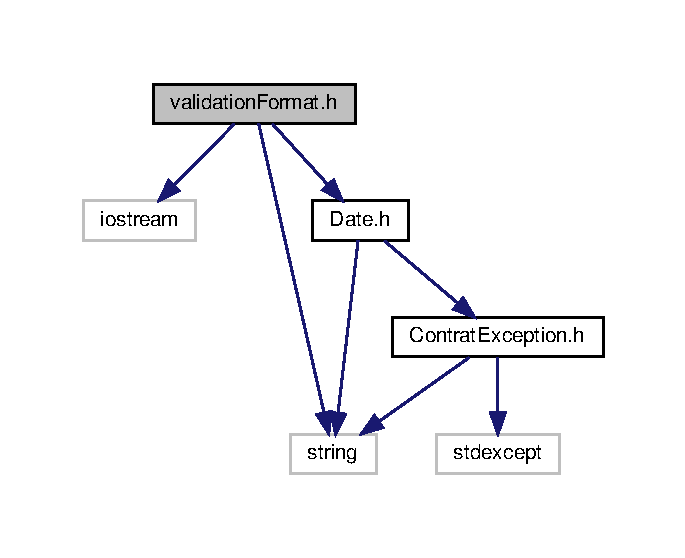
\includegraphics[width=329pt]{validationFormat_8h__incl}
\end{center}
\end{figure}
This graph shows which files directly or indirectly include this file\+:\nopagebreak
\begin{figure}[H]
\begin{center}
\leavevmode
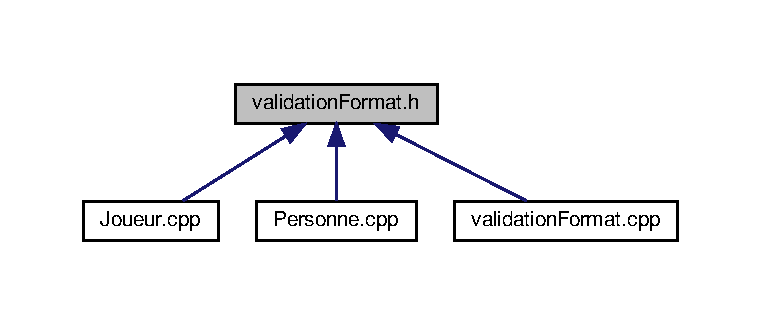
\includegraphics[width=350pt]{validationFormat_8h__dep__incl}
\end{center}
\end{figure}
\subsection*{Functions}
\begin{DoxyCompactItemize}
\item 
bool \hyperlink{validationFormat_8cpp_ad19b58e0318b66129069390b2da7496e}{util\+::valider\+Telephone} (const std\+::string \&p\+\_\+telephone)
\begin{DoxyCompactList}\small\item\em Valide le format d\textquotesingle{}un numéro de téléphone pour qu\textquotesingle{}il respecte le format national canadien standard. \end{DoxyCompactList}\item 
bool \hyperlink{validationFormat_8cpp_a5743386c1cc811ee37f66a9c58162ff5}{util\+::verification\+Longueur\+Tel} (const std\+::string \&p\+\_\+telephone)
\begin{DoxyCompactList}\small\item\em Vérifie que le string du numéro de téléphone est de la bonne longueur. \end{DoxyCompactList}\item 
bool \hyperlink{validationFormat_8cpp_a91d98db549a5328db80783a9cb5a3811}{util\+::verification\+Espace\+Trait} (const std\+::string \&p\+\_\+telephone)
\begin{DoxyCompactList}\small\item\em Vérifie que le numéro contient un espace et un trait et qu\textquotesingle{}ils sont aux bons endroits. \end{DoxyCompactList}\item 
bool \hyperlink{validationFormat_8cpp_a00b57c98b926a63daa8215e1436b63dc}{util\+::verification\+Chiffres} (const std\+::string \&p\+\_\+telephone)
\begin{DoxyCompactList}\small\item\em Vérifie que le numéro ne contient que des chiffres (à l\textquotesingle{}exception de l\textquotesingle{}espace et du trait) \end{DoxyCompactList}\item 
bool \hyperlink{validationFormat_8cpp_a06d6b26422f8b93767e39482e237c75c}{util\+::verification\+Indicatif} (const std\+::string \&p\+\_\+telephone)
\begin{DoxyCompactList}\small\item\em Vérifie que l\textquotesingle{}indicatif du numéro est un indicatif valide. Pour ce faire le programme vérifie dans un tableau d\textquotesingle{}indicatifs acceptés I\+N\+D\+I\+C\+A\+T\+I\+F\+S\+\_\+\+A\+C\+C\+E\+P\+T\+ES\mbox{[}\mbox{]} ou encore accepte l\textquotesingle{}indicatif s\textquotesingle{}il commence par un 9. \end{DoxyCompactList}\item 
bool \hyperlink{validationFormat_8cpp_a25f8d52b23785c48a5256d8b66ab466d}{util\+::valider\+Num\+R\+A\+MQ} (const std\+::string \&p\+\_\+numero, const std\+::string \&p\+\_\+nom, const std\+::string \&p\+\_\+prenom, int p\+\_\+jour\+Naissance, int p\+\_\+mois\+Naissance, int p\+\_\+annee\+Naissance, char p\+\_\+sexe)
\begin{DoxyCompactList}\small\item\em Vérifie qu\textquotesingle{}un numéro de R\+A\+MQ fourni sous forme de string respecte le format standard et qu\textquotesingle{}il concorde avec les autres informations fournies. Le format standard est les suivant N\+N\+NP A\+A\+MM J\+J\+XX où NN sont les trois premières lettres du nom de famille de la personne en Maj, P est la première lettre du prénom de la personne en Maj, AA sont les deux derniers chiffres de l\textquotesingle{}année de naissance de la personne MM sont les chiffres du mois de naissance de la personne JJ sont les chiffres du jour de naissance de la personne XX est un code administratif dont on ne connait pas la valeur. \end{DoxyCompactList}\item 
bool \hyperlink{validationFormat_8cpp_a79c9909ab5b1e969dc6b2f77d966eb6c}{util\+::verification\+Longueur\+R\+A\+MQ} (const std\+::string \&p\+\_\+numero)
\begin{DoxyCompactList}\small\item\em Vérifie que le numéro de la R\+A\+MQ fournie est de la bonne longueur. \end{DoxyCompactList}\item 
bool \hyperlink{validationFormat_8cpp_a6046ececaf0ad6874e7a9b76a797ff44}{util\+::verification\+Position\+Espaces\+R\+A\+MQ} (const std\+::string \&p\+\_\+numero)
\begin{DoxyCompactList}\small\item\em Vérifie que le numéro de la R\+A\+MQ fournie possède deux espaces qui sont aux bons endroits. \end{DoxyCompactList}\item 
bool \hyperlink{validationFormat_8cpp_a8515bea07b4b8021d249d03d6626b7ee}{util\+::verification\+Nom\+R\+A\+MQ} (const std\+::string \&p\+\_\+numero, const std\+::string \&p\+\_\+nom)
\begin{DoxyCompactList}\small\item\em Vérifie que le numéro de la R\+A\+MQ fournie concorde avec le nom de la personne. \end{DoxyCompactList}\item 
bool \hyperlink{validationFormat_8cpp_af22d126590f7a04264c228a2dc1f1dca}{util\+::verification\+Prenom\+R\+A\+MQ} (const std\+::string \&p\+\_\+numero, const std\+::string \&p\+\_\+prenom)
\begin{DoxyCompactList}\small\item\em Vérifie que le numéro de la R\+A\+MQ fournie concorde avec le prénom de la personne. \end{DoxyCompactList}\item 
bool \hyperlink{validationFormat_8cpp_ac1410e9900e443039e04492a9dcb51ae}{util\+::verification\+Annee\+R\+A\+MQ} (const std\+::string \&p\+\_\+numero, const int p\+\_\+annee\+Naissance)
\begin{DoxyCompactList}\small\item\em Vérifie que le numéro de la R\+A\+MQ fournie concorde avec l\textquotesingle{}année de naissance de la personne. \end{DoxyCompactList}\item 
bool \hyperlink{validationFormat_8cpp_a6b46e2eb29fab39a4b3df7c6c703b3b3}{util\+::verification\+Mois\+R\+A\+MQ} (const std\+::string \&p\+\_\+numero, const int p\+\_\+mois\+Naissance, char \&p\+\_\+sexe)
\begin{DoxyCompactList}\small\item\em Vérifie que le numéro de la R\+A\+MQ fournie concorde avec le mois de naissance de la personne. \end{DoxyCompactList}\item 
bool \hyperlink{validationFormat_8cpp_a9188427a80c9811cb9cac0432584a097}{util\+::verification\+Jour\+R\+A\+MQ} (const std\+::string \&p\+\_\+numero, int p\+\_\+jour\+Naissance)
\begin{DoxyCompactList}\small\item\em Vérifie que le numéro de la R\+A\+MQ fournie concorde avec le jour de naissance de la personne. \end{DoxyCompactList}\item 
std\+::string \hyperlink{validationFormat_8cpp_a9725447dd2572abb047af57c0101793f}{util\+::transfo\+Majuscule} (const std\+::string \&p\+\_\+chaine\+A\+Changer)
\begin{DoxyCompactList}\small\item\em Fonction qui prend un string en entrée et donne en sortie un string majuscule du string d\textquotesingle{}entrée. \end{DoxyCompactList}\item 
bool \hyperlink{validationFormat_8cpp_ab3d93e73408df98688844f00a8cdce58}{util\+::valider\+Format\+Nom} (const std\+::string \&p\+\_\+nom)
\begin{DoxyCompactList}\small\item\em Vérifie que le nom donné ne contient que des lettres (maj ou min) et n\textquotesingle{}est pas vide. \end{DoxyCompactList}\item 
bool \hyperlink{validationFormat_8cpp_a0f4b6c8097b37ec3712dc34d2363a083}{util\+::valider\+Sexe} (const char \&p\+\_\+sexe)
\begin{DoxyCompactList}\small\item\em Vérifie que le sexe donné en entrée est soit \textquotesingle{}M\textquotesingle{},\textquotesingle{}m\textquotesingle{},\textquotesingle{}F\textquotesingle{} ou \textquotesingle{}f\textquotesingle{}. \end{DoxyCompactList}\item 
bool \hyperlink{validationFormat_8cpp_afc8b13ca75c2d31a81d2cff1e9ae7d7c}{util\+::valider\+Position} (const std\+::string \&p\+\_\+position)
\begin{DoxyCompactList}\small\item\em Vérifie que la position en entrée est soit \char`\"{}centre\char`\"{},\char`\"{}ailier\char`\"{},\char`\"{}défenseur\char`\"{} ou \char`\"{}gardien\char`\"{}. \end{DoxyCompactList}\item 
bool \hyperlink{validationFormat_8cpp_abed031230a6601feb893f74fe783c5ff}{util\+::valider\+Age\+Entraineur} (const Date \&p\+\_\+date\+Naissance\+Entraineur)
\begin{DoxyCompactList}\small\item\em Vérifie que l\textquotesingle{}âge en entrée est supérieur à 18 ans. \end{DoxyCompactList}\item 
bool \hyperlink{validationFormat_8cpp_afef869875a75ed592e94ef4f02d08419}{util\+::valider\+Age\+Joueur} (const Date \&p\+\_\+date\+Naissance\+Joueur)
\begin{DoxyCompactList}\small\item\em Vérifie que l\textquotesingle{}âge en entrée est entre 15 et 17 ans. \end{DoxyCompactList}\end{DoxyCompactItemize}


\subsection{Detailed Description}
Fichier de déclaration des constantes et des fonctions pour la validation. 

\begin{DoxyAuthor}{Author}
Jordan Longval 
\end{DoxyAuthor}
\begin{DoxyVersion}{Version}
1.\+0 
\end{DoxyVersion}
\begin{DoxyDate}{Date}
10/02/20 
\end{DoxyDate}


\subsection{Function Documentation}
\mbox{\Hypertarget{validationFormat_8cpp_file_a9725447dd2572abb047af57c0101793f}\label{validationFormat_8cpp_file_a9725447dd2572abb047af57c0101793f}} 
\index{validation\+Format.\+h@{validation\+Format.\+h}!transfo\+Majuscule@{transfo\+Majuscule}}
\index{transfo\+Majuscule@{transfo\+Majuscule}!validation\+Format.\+h@{validation\+Format.\+h}}
\subsubsection{\texorpdfstring{transfo\+Majuscule()}{transfoMajuscule()}}
{\footnotesize\ttfamily std\+::string util\+::transfo\+Majuscule (\begin{DoxyParamCaption}\item[{const std\+::string \&}]{p\+\_\+chaine\+A\+Changer }\end{DoxyParamCaption})}



Fonction qui prend un string en entrée et donne en sortie un string majuscule du string d\textquotesingle{}entrée. 


\begin{DoxyParams}[1]{Parameters}
\mbox{\tt in}  & {\em p\+\_\+chaine\+A\+Changer} & un string que l\textquotesingle{}on veut mettre complètement en majuscule \\
\hline
\end{DoxyParams}
\begin{DoxyPrecond}{Precondition}
p\+\_\+chaine\+A\+Changer ne doit contenir que des lettres de a à z ou A à Z. 
\end{DoxyPrecond}
\begin{DoxyReturn}{Returns}
un string contenant la version majuscule de la chaine à changer. 
\end{DoxyReturn}
\mbox{\Hypertarget{validationFormat_8cpp_file_abed031230a6601feb893f74fe783c5ff}\label{validationFormat_8cpp_file_abed031230a6601feb893f74fe783c5ff}} 
\index{validation\+Format.\+h@{validation\+Format.\+h}!valider\+Age\+Entraineur@{valider\+Age\+Entraineur}}
\index{valider\+Age\+Entraineur@{valider\+Age\+Entraineur}!validation\+Format.\+h@{validation\+Format.\+h}}
\subsubsection{\texorpdfstring{valider\+Age\+Entraineur()}{validerAgeEntraineur()}}
{\footnotesize\ttfamily bool util\+::valider\+Age\+Entraineur (\begin{DoxyParamCaption}\item[{const \hyperlink{classutil_1_1Date}{Date} \&}]{p\+\_\+date\+Naissance\+Entraineur }\end{DoxyParamCaption})}



Vérifie que l\textquotesingle{}âge en entrée est supérieur à 18 ans. 


\begin{DoxyParams}[1]{Parameters}
\mbox{\tt in}  & {\em p\+\_\+date\+Naissance\+Entraineur} & la date de naissance à valider \\
\hline
\end{DoxyParams}
\begin{DoxyReturn}{Returns}
un bool qui est vrai lorsque les conditions sont satisfaites. 
\end{DoxyReturn}
\mbox{\Hypertarget{validationFormat_8cpp_file_afef869875a75ed592e94ef4f02d08419}\label{validationFormat_8cpp_file_afef869875a75ed592e94ef4f02d08419}} 
\index{validation\+Format.\+h@{validation\+Format.\+h}!valider\+Age\+Joueur@{valider\+Age\+Joueur}}
\index{valider\+Age\+Joueur@{valider\+Age\+Joueur}!validation\+Format.\+h@{validation\+Format.\+h}}
\subsubsection{\texorpdfstring{valider\+Age\+Joueur()}{validerAgeJoueur()}}
{\footnotesize\ttfamily bool util\+::valider\+Age\+Joueur (\begin{DoxyParamCaption}\item[{const \hyperlink{classutil_1_1Date}{Date} \&}]{p\+\_\+date\+Naissance\+Joueur }\end{DoxyParamCaption})}



Vérifie que l\textquotesingle{}âge en entrée est entre 15 et 17 ans. 


\begin{DoxyParams}[1]{Parameters}
\mbox{\tt in}  & {\em p\+\_\+date\+Naissance\+Joueur} & la date de naissance à valider \\
\hline
\end{DoxyParams}
\begin{DoxyReturn}{Returns}
un bool qui est vrai lorsque les conditions sont satisfaites. 
\end{DoxyReturn}
\mbox{\Hypertarget{validationFormat_8cpp_file_ab3d93e73408df98688844f00a8cdce58}\label{validationFormat_8cpp_file_ab3d93e73408df98688844f00a8cdce58}} 
\index{validation\+Format.\+h@{validation\+Format.\+h}!valider\+Format\+Nom@{valider\+Format\+Nom}}
\index{valider\+Format\+Nom@{valider\+Format\+Nom}!validation\+Format.\+h@{validation\+Format.\+h}}
\subsubsection{\texorpdfstring{valider\+Format\+Nom()}{validerFormatNom()}}
{\footnotesize\ttfamily bool util\+::valider\+Format\+Nom (\begin{DoxyParamCaption}\item[{const std\+::string \&}]{p\+\_\+nom }\end{DoxyParamCaption})}



Vérifie que le nom donné ne contient que des lettres (maj ou min) et n\textquotesingle{}est pas vide. 


\begin{DoxyParams}[1]{Parameters}
\mbox{\tt in}  & {\em p\+\_\+nom} & le nom à valider \\
\hline
\end{DoxyParams}
\begin{DoxyReturn}{Returns}
un bool qui est vrai lorsque le nom de contient que des lettres (Maj ou min) et n\textquotesingle{}est pas vide et faux si ce n\textquotesingle{}est pas le cas. 
\end{DoxyReturn}
\mbox{\Hypertarget{validationFormat_8cpp_file_a25f8d52b23785c48a5256d8b66ab466d}\label{validationFormat_8cpp_file_a25f8d52b23785c48a5256d8b66ab466d}} 
\index{validation\+Format.\+h@{validation\+Format.\+h}!valider\+Num\+R\+A\+MQ@{valider\+Num\+R\+A\+MQ}}
\index{valider\+Num\+R\+A\+MQ@{valider\+Num\+R\+A\+MQ}!validation\+Format.\+h@{validation\+Format.\+h}}
\subsubsection{\texorpdfstring{valider\+Num\+R\+A\+M\+Q()}{validerNumRAMQ()}}
{\footnotesize\ttfamily bool util\+::valider\+Num\+R\+A\+MQ (\begin{DoxyParamCaption}\item[{const std\+::string \&}]{p\+\_\+numero,  }\item[{const std\+::string \&}]{p\+\_\+nom,  }\item[{const std\+::string \&}]{p\+\_\+prenom,  }\item[{int}]{p\+\_\+jour\+Naissance,  }\item[{int}]{p\+\_\+mois\+Naissance,  }\item[{int}]{p\+\_\+annee\+Naissance,  }\item[{char}]{p\+\_\+sexe }\end{DoxyParamCaption})}



Vérifie qu\textquotesingle{}un numéro de R\+A\+MQ fourni sous forme de string respecte le format standard et qu\textquotesingle{}il concorde avec les autres informations fournies. Le format standard est les suivant N\+N\+NP A\+A\+MM J\+J\+XX où NN sont les trois premières lettres du nom de famille de la personne en Maj, P est la première lettre du prénom de la personne en Maj, AA sont les deux derniers chiffres de l\textquotesingle{}année de naissance de la personne MM sont les chiffres du mois de naissance de la personne JJ sont les chiffres du jour de naissance de la personne XX est un code administratif dont on ne connait pas la valeur. 


\begin{DoxyParams}[1]{Parameters}
\mbox{\tt in}  & {\em p\+\_\+numero} & Un string contenant le numéro de R\+A\+MQ à valider \\
\hline
\mbox{\tt in}  & {\em p\+\_\+nom} & Un string contenant le nom de la personne \\
\hline
\mbox{\tt in}  & {\em p\+\_\+prenom} & Un string contenant le prenom de la personne \\
\hline
\mbox{\tt in}  & {\em p\+\_\+jour\+Naissance} & un entier représentant le jour de naissance de la personne \\
\hline
\mbox{\tt in}  & {\em p\+\_\+mois\+Naissance} & un entier représentant le mois de naissance de la personne \\
\hline
\mbox{\tt in}  & {\em p\+\_\+annee\+Naissance} & un entier représentant les deux derniers chiffres de l\textquotesingle{}année de naissance de la personne \\
\hline
\mbox{\tt in}  & {\em p\+\_\+sexe} & un charactère représentant le sexe de la personne \\
\hline
\end{DoxyParams}
\begin{DoxyPrecond}{Precondition}
les valeurs p\+\_\+nom à p\+\_\+sex doivent être valides. les valeurs valides de p\+\_\+sex sont \textquotesingle{}m\textquotesingle{},\textquotesingle{}M\textquotesingle{},pour homme et \textquotesingle{}f\textquotesingle{},\textquotesingle{}F\textquotesingle{}, pour femme. 
\end{DoxyPrecond}
\begin{DoxyReturn}{Returns}
un bool qui est vrai lorsque le numéro de R\+A\+MQ est valide. et faux si ce n\textquotesingle{}est pas le cas. 
\end{DoxyReturn}
\mbox{\Hypertarget{validationFormat_8cpp_file_afc8b13ca75c2d31a81d2cff1e9ae7d7c}\label{validationFormat_8cpp_file_afc8b13ca75c2d31a81d2cff1e9ae7d7c}} 
\index{validation\+Format.\+h@{validation\+Format.\+h}!valider\+Position@{valider\+Position}}
\index{valider\+Position@{valider\+Position}!validation\+Format.\+h@{validation\+Format.\+h}}
\subsubsection{\texorpdfstring{valider\+Position()}{validerPosition()}}
{\footnotesize\ttfamily bool util\+::valider\+Position (\begin{DoxyParamCaption}\item[{const std\+::string \&}]{p\+\_\+position }\end{DoxyParamCaption})}



Vérifie que la position en entrée est soit \char`\"{}centre\char`\"{},\char`\"{}ailier\char`\"{},\char`\"{}défenseur\char`\"{} ou \char`\"{}gardien\char`\"{}. 


\begin{DoxyParams}[1]{Parameters}
\mbox{\tt in}  & {\em p\+\_\+position} & la position à valider \\
\hline
\end{DoxyParams}
\begin{DoxyReturn}{Returns}
un bool qui est vrai lorsque les conditions sont satisfaites. 
\end{DoxyReturn}
\mbox{\Hypertarget{validationFormat_8cpp_file_a0f4b6c8097b37ec3712dc34d2363a083}\label{validationFormat_8cpp_file_a0f4b6c8097b37ec3712dc34d2363a083}} 
\index{validation\+Format.\+h@{validation\+Format.\+h}!valider\+Sexe@{valider\+Sexe}}
\index{valider\+Sexe@{valider\+Sexe}!validation\+Format.\+h@{validation\+Format.\+h}}
\subsubsection{\texorpdfstring{valider\+Sexe()}{validerSexe()}}
{\footnotesize\ttfamily bool util\+::valider\+Sexe (\begin{DoxyParamCaption}\item[{const char \&}]{p\+\_\+sexe }\end{DoxyParamCaption})}



Vérifie que le sexe donné en entrée est soit \textquotesingle{}M\textquotesingle{},\textquotesingle{}m\textquotesingle{},\textquotesingle{}F\textquotesingle{} ou \textquotesingle{}f\textquotesingle{}. 


\begin{DoxyParams}[1]{Parameters}
\mbox{\tt in}  & {\em p\+\_\+sexe} & le sexe à valider \\
\hline
\end{DoxyParams}
\begin{DoxyReturn}{Returns}
un bool qui est vrai lorsque les conditions sont satisfaites. 
\end{DoxyReturn}
\mbox{\Hypertarget{validationFormat_8cpp_file_ad19b58e0318b66129069390b2da7496e}\label{validationFormat_8cpp_file_ad19b58e0318b66129069390b2da7496e}} 
\index{validation\+Format.\+h@{validation\+Format.\+h}!valider\+Telephone@{valider\+Telephone}}
\index{valider\+Telephone@{valider\+Telephone}!validation\+Format.\+h@{validation\+Format.\+h}}
\subsubsection{\texorpdfstring{valider\+Telephone()}{validerTelephone()}}
{\footnotesize\ttfamily bool util\+::valider\+Telephone (\begin{DoxyParamCaption}\item[{const std\+::string \&}]{p\+\_\+telephone }\end{DoxyParamCaption})}



Valide le format d\textquotesingle{}un numéro de téléphone pour qu\textquotesingle{}il respecte le format national canadien standard. 


\begin{DoxyParams}[1]{Parameters}
\mbox{\tt in}  & {\em p\+\_\+telephone} & Un string contenant le numéro de téléphone à valider. \\
\hline
\end{DoxyParams}
\begin{DoxyPrecond}{Precondition}
p\+\_\+telephone doit être une variable std\+::string. 
\end{DoxyPrecond}
\begin{DoxyReturn}{Returns}
un bool qui est vrai lorsque le numéro respecte le format et faux si ce n\textquotesingle{}est pas le cas. 
\end{DoxyReturn}
\mbox{\Hypertarget{validationFormat_8cpp_file_ac1410e9900e443039e04492a9dcb51ae}\label{validationFormat_8cpp_file_ac1410e9900e443039e04492a9dcb51ae}} 
\index{validation\+Format.\+h@{validation\+Format.\+h}!verification\+Annee\+R\+A\+MQ@{verification\+Annee\+R\+A\+MQ}}
\index{verification\+Annee\+R\+A\+MQ@{verification\+Annee\+R\+A\+MQ}!validation\+Format.\+h@{validation\+Format.\+h}}
\subsubsection{\texorpdfstring{verification\+Annee\+R\+A\+M\+Q()}{verificationAnneeRAMQ()}}
{\footnotesize\ttfamily bool util\+::verification\+Annee\+R\+A\+MQ (\begin{DoxyParamCaption}\item[{const std\+::string \&}]{p\+\_\+numero,  }\item[{const int}]{p\+\_\+annee\+Naissance }\end{DoxyParamCaption})}



Vérifie que le numéro de la R\+A\+MQ fournie concorde avec l\textquotesingle{}année de naissance de la personne. 


\begin{DoxyParams}[1]{Parameters}
\mbox{\tt in}  & {\em p\+\_\+numero} & Le string du numéro de la R\+A\+MQ fourni \\
\hline
\mbox{\tt in}  & {\em p\+\_\+annee\+Naissance} & un int contenant l\textquotesingle{}annee de naissance de la personne \\
\hline
\end{DoxyParams}
\begin{DoxyPrecond}{Precondition}
p\+\_\+numero doit être un string 

p\+\_\+annee\+Naissance doit être un int et l\textquotesingle{}année de naissance doit être valide. 
\end{DoxyPrecond}
\begin{DoxyReturn}{Returns}
un bool qui est vrai lorsque le numéro de la R\+A\+MQ concorde avec l\textquotesingle{}année de naissance de la personne et faux si ce n\textquotesingle{}est pas le cas. 
\end{DoxyReturn}
\mbox{\Hypertarget{validationFormat_8cpp_file_a00b57c98b926a63daa8215e1436b63dc}\label{validationFormat_8cpp_file_a00b57c98b926a63daa8215e1436b63dc}} 
\index{validation\+Format.\+h@{validation\+Format.\+h}!verification\+Chiffres@{verification\+Chiffres}}
\index{verification\+Chiffres@{verification\+Chiffres}!validation\+Format.\+h@{validation\+Format.\+h}}
\subsubsection{\texorpdfstring{verification\+Chiffres()}{verificationChiffres()}}
{\footnotesize\ttfamily bool util\+::verification\+Chiffres (\begin{DoxyParamCaption}\item[{const std\+::string \&}]{p\+\_\+telephone }\end{DoxyParamCaption})}



Vérifie que le numéro ne contient que des chiffres (à l\textquotesingle{}exception de l\textquotesingle{}espace et du trait) 


\begin{DoxyParams}[1]{Parameters}
\mbox{\tt in}  & {\em p\+\_\+telephone} & Un string contenant le numéro de téléphone à valider. \\
\hline
\end{DoxyParams}
\begin{DoxyPrecond}{Precondition}
p\+\_\+telephone doit être une variable std\+::string qui a passé toutes les validations des fonctions précédentes. 
\end{DoxyPrecond}
\begin{DoxyReturn}{Returns}
un bool qui est vrai lorsque le numéro ne contient que des chiffres et faux si ce n\textquotesingle{}est pas le cas. 
\end{DoxyReturn}
\mbox{\Hypertarget{validationFormat_8cpp_file_a91d98db549a5328db80783a9cb5a3811}\label{validationFormat_8cpp_file_a91d98db549a5328db80783a9cb5a3811}} 
\index{validation\+Format.\+h@{validation\+Format.\+h}!verification\+Espace\+Trait@{verification\+Espace\+Trait}}
\index{verification\+Espace\+Trait@{verification\+Espace\+Trait}!validation\+Format.\+h@{validation\+Format.\+h}}
\subsubsection{\texorpdfstring{verification\+Espace\+Trait()}{verificationEspaceTrait()}}
{\footnotesize\ttfamily bool util\+::verification\+Espace\+Trait (\begin{DoxyParamCaption}\item[{const std\+::string \&}]{p\+\_\+telephone }\end{DoxyParamCaption})}



Vérifie que le numéro contient un espace et un trait et qu\textquotesingle{}ils sont aux bons endroits. 


\begin{DoxyParams}[1]{Parameters}
\mbox{\tt in}  & {\em p\+\_\+telephone} & Un string contenant le numéro de téléphone à valider. \\
\hline
\end{DoxyParams}
\begin{DoxyPrecond}{Precondition}
p\+\_\+telephone doit être une variable std\+::string qui a passé toutes les validations des fonctions précédentes. 
\end{DoxyPrecond}
\begin{DoxyReturn}{Returns}
un bool qui est vrai lorsque l\textquotesingle{}espace et le trait sont présents et aux bons endroits et faux si ce n\textquotesingle{}est pas le cas. 
\end{DoxyReturn}
\mbox{\Hypertarget{validationFormat_8cpp_file_a06d6b26422f8b93767e39482e237c75c}\label{validationFormat_8cpp_file_a06d6b26422f8b93767e39482e237c75c}} 
\index{validation\+Format.\+h@{validation\+Format.\+h}!verification\+Indicatif@{verification\+Indicatif}}
\index{verification\+Indicatif@{verification\+Indicatif}!validation\+Format.\+h@{validation\+Format.\+h}}
\subsubsection{\texorpdfstring{verification\+Indicatif()}{verificationIndicatif()}}
{\footnotesize\ttfamily bool util\+::verification\+Indicatif (\begin{DoxyParamCaption}\item[{const std\+::string \&}]{p\+\_\+telephone }\end{DoxyParamCaption})}



Vérifie que l\textquotesingle{}indicatif du numéro est un indicatif valide. Pour ce faire le programme vérifie dans un tableau d\textquotesingle{}indicatifs acceptés I\+N\+D\+I\+C\+A\+T\+I\+F\+S\+\_\+\+A\+C\+C\+E\+P\+T\+ES\mbox{[}\mbox{]} ou encore accepte l\textquotesingle{}indicatif s\textquotesingle{}il commence par un 9. 


\begin{DoxyParams}[1]{Parameters}
\mbox{\tt in}  & {\em p\+\_\+telephone} & Un string contenant le numéro de téléphone à valider. \\
\hline
\end{DoxyParams}
\begin{DoxyPrecond}{Precondition}
p\+\_\+telephone doit être une variable std\+::string qui a passé toutes les validations des fonctions précédentes. 
\end{DoxyPrecond}
\begin{DoxyReturn}{Returns}
un bool qui est vrai lorsque le numéro a un indicatif valide. et faux si ce n\textquotesingle{}est pas le cas. 
\end{DoxyReturn}
\mbox{\Hypertarget{validationFormat_8cpp_file_a9188427a80c9811cb9cac0432584a097}\label{validationFormat_8cpp_file_a9188427a80c9811cb9cac0432584a097}} 
\index{validation\+Format.\+h@{validation\+Format.\+h}!verification\+Jour\+R\+A\+MQ@{verification\+Jour\+R\+A\+MQ}}
\index{verification\+Jour\+R\+A\+MQ@{verification\+Jour\+R\+A\+MQ}!validation\+Format.\+h@{validation\+Format.\+h}}
\subsubsection{\texorpdfstring{verification\+Jour\+R\+A\+M\+Q()}{verificationJourRAMQ()}}
{\footnotesize\ttfamily bool util\+::verification\+Jour\+R\+A\+MQ (\begin{DoxyParamCaption}\item[{const std\+::string \&}]{p\+\_\+numero,  }\item[{int}]{p\+\_\+jour\+Naissance }\end{DoxyParamCaption})}



Vérifie que le numéro de la R\+A\+MQ fournie concorde avec le jour de naissance de la personne. 


\begin{DoxyParams}[1]{Parameters}
\mbox{\tt in}  & {\em p\+\_\+numero} & Le string du numéro de la R\+A\+MQ fourni \\
\hline
\mbox{\tt in}  & {\em p\+\_\+jour\+Naissance} & un int contenant le jour de naissance de la personne \\
\hline
\end{DoxyParams}
\begin{DoxyPrecond}{Precondition}
p\+\_\+numero doit être un string 

p\+\_\+jour\+Naissance doit être un int et le jour de naissance doit être valide. 
\end{DoxyPrecond}
\begin{DoxyReturn}{Returns}
un bool qui est vrai lorsque le numéro de la R\+A\+MQ concorde avec le jour de naissance de la personne et faux si ce n\textquotesingle{}est pas le cas. 
\end{DoxyReturn}
\mbox{\Hypertarget{validationFormat_8cpp_file_a79c9909ab5b1e969dc6b2f77d966eb6c}\label{validationFormat_8cpp_file_a79c9909ab5b1e969dc6b2f77d966eb6c}} 
\index{validation\+Format.\+h@{validation\+Format.\+h}!verification\+Longueur\+R\+A\+MQ@{verification\+Longueur\+R\+A\+MQ}}
\index{verification\+Longueur\+R\+A\+MQ@{verification\+Longueur\+R\+A\+MQ}!validation\+Format.\+h@{validation\+Format.\+h}}
\subsubsection{\texorpdfstring{verification\+Longueur\+R\+A\+M\+Q()}{verificationLongueurRAMQ()}}
{\footnotesize\ttfamily bool util\+::verification\+Longueur\+R\+A\+MQ (\begin{DoxyParamCaption}\item[{const std\+::string \&}]{p\+\_\+numero }\end{DoxyParamCaption})}



Vérifie que le numéro de la R\+A\+MQ fournie est de la bonne longueur. 


\begin{DoxyParams}[1]{Parameters}
\mbox{\tt in}  & {\em p\+\_\+numero} & Le string du numéro de la R\+A\+MQ fourni. \\
\hline
\end{DoxyParams}
\begin{DoxyPrecond}{Precondition}
p\+\_\+numero doit être un string 
\end{DoxyPrecond}
\begin{DoxyReturn}{Returns}
un bool qui est vrai lorsque le numéro est de la bonne longueur et faux si ce n\textquotesingle{}est pas le cas. 
\end{DoxyReturn}
\mbox{\Hypertarget{validationFormat_8cpp_file_a5743386c1cc811ee37f66a9c58162ff5}\label{validationFormat_8cpp_file_a5743386c1cc811ee37f66a9c58162ff5}} 
\index{validation\+Format.\+h@{validation\+Format.\+h}!verification\+Longueur\+Tel@{verification\+Longueur\+Tel}}
\index{verification\+Longueur\+Tel@{verification\+Longueur\+Tel}!validation\+Format.\+h@{validation\+Format.\+h}}
\subsubsection{\texorpdfstring{verification\+Longueur\+Tel()}{verificationLongueurTel()}}
{\footnotesize\ttfamily bool util\+::verification\+Longueur\+Tel (\begin{DoxyParamCaption}\item[{const std\+::string \&}]{p\+\_\+telephone }\end{DoxyParamCaption})}



Vérifie que le string du numéro de téléphone est de la bonne longueur. 


\begin{DoxyParams}[1]{Parameters}
\mbox{\tt in}  & {\em p\+\_\+telephone} & Un string contenant le numéro de téléphone à valider. \\
\hline
\end{DoxyParams}
\begin{DoxyPrecond}{Precondition}
p\+\_\+telephone doit être une variable std\+::string. 
\end{DoxyPrecond}
\begin{DoxyReturn}{Returns}
un bool qui est vrai lorsque le numéro est de la bonne longueur et faux si ce n\textquotesingle{}est pas le cas. 
\end{DoxyReturn}
\mbox{\Hypertarget{validationFormat_8cpp_file_a6b46e2eb29fab39a4b3df7c6c703b3b3}\label{validationFormat_8cpp_file_a6b46e2eb29fab39a4b3df7c6c703b3b3}} 
\index{validation\+Format.\+h@{validation\+Format.\+h}!verification\+Mois\+R\+A\+MQ@{verification\+Mois\+R\+A\+MQ}}
\index{verification\+Mois\+R\+A\+MQ@{verification\+Mois\+R\+A\+MQ}!validation\+Format.\+h@{validation\+Format.\+h}}
\subsubsection{\texorpdfstring{verification\+Mois\+R\+A\+M\+Q()}{verificationMoisRAMQ()}}
{\footnotesize\ttfamily bool util\+::verification\+Mois\+R\+A\+MQ (\begin{DoxyParamCaption}\item[{const std\+::string \&}]{p\+\_\+numero,  }\item[{const int}]{p\+\_\+mois\+Naissance,  }\item[{char \&}]{p\+\_\+sexe }\end{DoxyParamCaption})}



Vérifie que le numéro de la R\+A\+MQ fournie concorde avec le mois de naissance de la personne. 


\begin{DoxyParams}[1]{Parameters}
\mbox{\tt in}  & {\em p\+\_\+numero} & Le string du numéro de la R\+A\+MQ fourni \\
\hline
\mbox{\tt in}  & {\em p\+\_\+mois\+Naissance} & un int contenant le mois de naissance de la personne \\
\hline
\mbox{\tt in}  & {\em p\+\_\+sexe} & un char représentant le sexe de la personne. \\
\hline
\end{DoxyParams}
\begin{DoxyPrecond}{Precondition}
p\+\_\+numero doit être un string 

p\+\_\+mois\+Naissance doit être un int et le mois de naissance doit être valide. 

p\+\_\+sexe doit être un char valant \textquotesingle{}m\textquotesingle{},\textquotesingle{}M\textquotesingle{},\textquotesingle{}f\textquotesingle{} ou \textquotesingle{}F\textquotesingle{} et le sexe de la personne doit être valide. 
\end{DoxyPrecond}
\begin{DoxyReturn}{Returns}
un bool qui est vrai lorsque le numéro de la R\+A\+MQ concorde avec le mois de naissance de la personne et faux si ce n\textquotesingle{}est pas le cas. 
\end{DoxyReturn}
\mbox{\Hypertarget{validationFormat_8cpp_file_a8515bea07b4b8021d249d03d6626b7ee}\label{validationFormat_8cpp_file_a8515bea07b4b8021d249d03d6626b7ee}} 
\index{validation\+Format.\+h@{validation\+Format.\+h}!verification\+Nom\+R\+A\+MQ@{verification\+Nom\+R\+A\+MQ}}
\index{verification\+Nom\+R\+A\+MQ@{verification\+Nom\+R\+A\+MQ}!validation\+Format.\+h@{validation\+Format.\+h}}
\subsubsection{\texorpdfstring{verification\+Nom\+R\+A\+M\+Q()}{verificationNomRAMQ()}}
{\footnotesize\ttfamily bool util\+::verification\+Nom\+R\+A\+MQ (\begin{DoxyParamCaption}\item[{const std\+::string \&}]{p\+\_\+numero,  }\item[{const std\+::string \&}]{p\+\_\+nom }\end{DoxyParamCaption})}



Vérifie que le numéro de la R\+A\+MQ fournie concorde avec le nom de la personne. 


\begin{DoxyParams}[1]{Parameters}
\mbox{\tt in}  & {\em p\+\_\+numero} & Le string du numéro de la R\+A\+MQ fourni \\
\hline
\mbox{\tt in}  & {\em p\+\_\+nom} & un string contenant le nom de la personne \\
\hline
\end{DoxyParams}
\begin{DoxyPrecond}{Precondition}
p\+\_\+numero doit être un string 

p\+\_\+nom doit être un string et le nom doit être valide. 
\end{DoxyPrecond}
\begin{DoxyReturn}{Returns}
un bool qui est vrai lorsque le numéro de la R\+A\+MQ concorde avec le nom de la personne et faux si ce n\textquotesingle{}est pas le cas. 
\end{DoxyReturn}
\mbox{\Hypertarget{validationFormat_8cpp_file_a6046ececaf0ad6874e7a9b76a797ff44}\label{validationFormat_8cpp_file_a6046ececaf0ad6874e7a9b76a797ff44}} 
\index{validation\+Format.\+h@{validation\+Format.\+h}!verification\+Position\+Espaces\+R\+A\+MQ@{verification\+Position\+Espaces\+R\+A\+MQ}}
\index{verification\+Position\+Espaces\+R\+A\+MQ@{verification\+Position\+Espaces\+R\+A\+MQ}!validation\+Format.\+h@{validation\+Format.\+h}}
\subsubsection{\texorpdfstring{verification\+Position\+Espaces\+R\+A\+M\+Q()}{verificationPositionEspacesRAMQ()}}
{\footnotesize\ttfamily bool util\+::verification\+Position\+Espaces\+R\+A\+MQ (\begin{DoxyParamCaption}\item[{const std\+::string \&}]{p\+\_\+numero }\end{DoxyParamCaption})}



Vérifie que le numéro de la R\+A\+MQ fournie possède deux espaces qui sont aux bons endroits. 


\begin{DoxyParams}[1]{Parameters}
\mbox{\tt in}  & {\em p\+\_\+numero} & Le string du numéro de la R\+A\+MQ fourni \\
\hline
\end{DoxyParams}
\begin{DoxyPrecond}{Precondition}
p\+\_\+numero doit être un string 
\end{DoxyPrecond}
\begin{DoxyReturn}{Returns}
un bool qui est vrai lorsque les espaces sont présents et aux bons endroits et faux si ce n\textquotesingle{}est pas le cas. 
\end{DoxyReturn}
\mbox{\Hypertarget{validationFormat_8cpp_file_af22d126590f7a04264c228a2dc1f1dca}\label{validationFormat_8cpp_file_af22d126590f7a04264c228a2dc1f1dca}} 
\index{validation\+Format.\+h@{validation\+Format.\+h}!verification\+Prenom\+R\+A\+MQ@{verification\+Prenom\+R\+A\+MQ}}
\index{verification\+Prenom\+R\+A\+MQ@{verification\+Prenom\+R\+A\+MQ}!validation\+Format.\+h@{validation\+Format.\+h}}
\subsubsection{\texorpdfstring{verification\+Prenom\+R\+A\+M\+Q()}{verificationPrenomRAMQ()}}
{\footnotesize\ttfamily bool util\+::verification\+Prenom\+R\+A\+MQ (\begin{DoxyParamCaption}\item[{const std\+::string \&}]{p\+\_\+numero,  }\item[{const std\+::string \&}]{p\+\_\+prenom }\end{DoxyParamCaption})}



Vérifie que le numéro de la R\+A\+MQ fournie concorde avec le prénom de la personne. 


\begin{DoxyParams}[1]{Parameters}
\mbox{\tt in}  & {\em p\+\_\+numero} & Le string du numéro de la R\+A\+MQ fourni \\
\hline
\mbox{\tt in}  & {\em p\+\_\+prenom} & un string contenant le nom de la personne \\
\hline
\end{DoxyParams}
\begin{DoxyPrecond}{Precondition}
p\+\_\+numero doit être un string 

p\+\_\+prenom doit être un string et le prenom doit être valide. 
\end{DoxyPrecond}
\begin{DoxyReturn}{Returns}
un bool qui est vrai lorsque le numéro de la R\+A\+MQ concorde avec le prenom de la personne et faux si ce n\textquotesingle{}est pas le cas. 
\end{DoxyReturn}

%--- End generated contents ---

% Index
\backmatter
\newpage
\phantomsection
\clearemptydoublepage
\addcontentsline{toc}{chapter}{Index}
\printindex

\end{document}
